\documentclass[10pt,a4paper]{article}
\usepackage[top=12mm,bottom=12mm,left=14mm,right=14mm]{geometry}
\usepackage{fontspec,xeCJK,xcolor,graphicx,tikz,hyperref,ragged2e}
\usetikzlibrary{calc,arrows.meta}
\setmainfont{Noto Sans}\setsansfont{Noto Sans}
\setCJKmainfont{Noto Sans CJK SC}\setCJKsansfont{Noto Sans CJK SC}
\definecolor{Paper}{HTML}{FCFAF7}\definecolor{Ink}{HTML}{2D3238}
\definecolor{Muted}{HTML}{70757A}\definecolor{Blue}{HTML}{5B9FBE}
\definecolor{Rose}{HTML}{B97589}\definecolor{Violet}{HTML}{8177A8}
\definecolor{Orange}{HTML}{D49757}\definecolor{Rule}{HTML}{DDE3E7}
\pagecolor{Paper}\color{Ink}\pagestyle{empty}
\setlength{\parindent}{0pt}\setlength{\parskip}{0pt}
\hypersetup{hidelinks,pdftitle={实验一过程报告：我与GPT的持续交互——改进工作流，完成实验一},pdfauthor={吴博闻},pdfsubject={真实Human–AI研究过程},bookmarksopen=true}
\newcommand{\PageStart}{\null\begin{tikzpicture}[remember picture,overlay]\begin{scope}[shift={(current page.north west)},x=1mm,y=-1mm]}
\newcommand{\PageEnd}{\end{scope}\end{tikzpicture}\clearpage}
\begin{document}
\PageStart
\node[anchor=north west,inner sep=0,text width=182.00mm,align=left] at (14.00,19.00) {\color{Rose}\fontsize{8.5}{11}\selectfont \bfseries SMART CITIES \& LOCATION SERVICES};
\node[anchor=north west,inner sep=0,text width=182.00mm,align=left] at (14.00,47.00) {\color{Ink}\fontsize{28}{35}\selectfont \bfseries 实验一过程报告};
\node[anchor=north west,inner sep=0,text width=182.00mm,align=left] at (14.00,72.00) {\color{Ink}\fontsize{18.5}{25}\selectfont \bfseries 我与 GPT 的持续交互：};
\node[anchor=north west,inner sep=0,text width=182.00mm,align=left] at (14.00,85.00) {\color{Ink}\fontsize{18.5}{25}\selectfont \bfseries 改进工作流，完成实验一};
\node[anchor=north west,inner sep=0,text width=176.00mm,align=left] at (14.00,116.00) {\color{Ink}\fontsize{10.7}{17}\selectfont  本报告记录我与 GPT 通过持续讨论、质疑、修改和核验，逐步完善协作工作流并完成实验一的过程。我们从既有协作经验出发，围绕任务理解、方法比较、实验反馈和报告表达调整做法；明确的工程任务交由 Codex 实现和运行，结果再回到讨论与核验中，推动后续决定。};
\draw[Blue,line width=1.1pt] (14,164)--(196,164);
\node[anchor=north west,inner sep=0,text width=176.00mm,align=left] at (14.00,181.00) {\color{Blue}\fontsize{11.5}{16}\selectfont \bfseries 截图采集};
\node[anchor=north west,inner sep=0,text width=176.00mm,align=left] at (14.00,194.00) {\color{Ink}\fontsize{10.7}{17}\selectfont  文档中的所有对话截图，都是我在 ChatGPT 网页中通过sharex软件利用长截图一张一张手动截取然后再利用图片分割器功能一张张切割并提供的；在本次协作中，GPT 没有直接截取我的网页对话界面的功能。};
\node[anchor=north west,inner sep=0,text width=170.00mm,align=left] at (14.00,258.00) {\color{Ink}\fontsize{11}{14}\selectfont \bfseries 吴博闻  ·  10245102410};
\draw[Rule,line width=.35pt] (14,283)--(196,283);
\node[anchor=north west,inner sep=0,text width=170.00mm,align=left] at (14.00,287.00) {\color{Muted}\fontsize{6.7}{8.5}\selectfont  智慧城市与位置服务  /  实验一过程报告};
\node[anchor=north west,inner sep=0,text width=11.00mm,align=left] at (185.00,286.50) {\color{Muted}\fontsize{8}{9}\selectfont  01};
\PageEnd

\PageStart
\node[anchor=north west,inner sep=0,text width=182.00mm,align=left] at (14.00,17.00) {\color{Ink}\fontsize{21}{27}\selectfont \bfseries 目录};
\node[anchor=north west,inner sep=0,text width=182.00mm,align=left] at (14.00,34.00) {\color{Ink}\fontsize{10}{15}\selectfont  先回看工作流的形成，再记录我与GPT推进实验一时的交互与决定。};
\node[anchor=north west,inner sep=0,text width=165.00mm,align=left] at (14.00,57.00) {\color{Rose}\fontsize{13}{18}\selectfont \bfseries Part I  工作流构建};
\node[anchor=north west,inner sep=0,text width=160.00mm,align=left] at (20.00,71.00) {\color{Ink}\fontsize{10.3}{15}\selectfont  协作方式的起点};
\node[anchor=north west,inner sep=0,text width=15.00mm,align=left] at (181.00,71.00) {\color{Muted}\fontsize{10.3}{15}\selectfont  3};
\node[anchor=north west,inner sep=0,text width=160.00mm,align=left] at (20.00,86.00) {\color{Ink}\fontsize{10.3}{15}\selectfont  范围与研究判断};
\node[anchor=north west,inner sep=0,text width=15.00mm,align=left] at (181.00,86.00) {\color{Muted}\fontsize{10.3}{15}\selectfont  5};
\node[anchor=north west,inner sep=0,text width=160.00mm,align=left] at (20.00,101.00) {\color{Ink}\fontsize{10.3}{15}\selectfont  报告与视觉表达};
\node[anchor=north west,inner sep=0,text width=15.00mm,align=left] at (181.00,101.00) {\color{Muted}\fontsize{10.3}{15}\selectfont  9};
\node[anchor=north west,inner sep=0,text width=160.00mm,align=left] at (20.00,116.00) {\color{Ink}\fontsize{10.3}{15}\selectfont  可追溯交付与研究入口};
\node[anchor=north west,inner sep=0,text width=15.00mm,align=left] at (181.00,116.00) {\color{Muted}\fontsize{10.3}{15}\selectfont  17};
\node[anchor=north west,inner sep=0,text width=165.00mm,align=left] at (14.00,140.00) {\color{Blue}\fontsize{13}{18}\selectfont \bfseries Part II  实验一中的交互与决策};
\node[anchor=north west,inner sep=0,text width=160.00mm,align=left] at (20.00,154.00) {\color{Ink}\fontsize{10.3}{15}\selectfont  任务理解与研究起点};
\node[anchor=north west,inner sep=0,text width=15.00mm,align=left] at (181.00,154.00) {\color{Muted}\fontsize{10.3}{15}\selectfont  21};
\node[anchor=north west,inner sep=0,text width=160.00mm,align=left] at (20.00,169.00) {\color{Ink}\fontsize{10.3}{15}\selectfont  面向实验任务的Multi-Agent构建};
\node[anchor=north west,inner sep=0,text width=15.00mm,align=left] at (181.00,169.00) {\color{Muted}\fontsize{10.3}{15}\selectfont  24};
\node[anchor=north west,inner sep=0,text width=160.00mm,align=left] at (20.00,184.00) {\color{Ink}\fontsize{10.3}{15}\selectfont  执行与审核机制的落地和修正};
\node[anchor=north west,inner sep=0,text width=15.00mm,align=left] at (181.00,184.00) {\color{Muted}\fontsize{10.3}{15}\selectfont  31};
\node[anchor=north west,inner sep=0,text width=160.00mm,align=left] at (20.00,199.00) {\color{Ink}\fontsize{10.3}{15}\selectfont  共同评价下的实验与AI建议检验};
\node[anchor=north west,inner sep=0,text width=15.00mm,align=left] at (181.00,199.00) {\color{Muted}\fontsize{10.3}{15}\selectfont  46};
\node[anchor=north west,inner sep=0,text width=160.00mm,align=left] at (20.00,214.00) {\color{Ink}\fontsize{10.3}{15}\selectfont  方案组合、回退与最终确认};
\node[anchor=north west,inner sep=0,text width=15.00mm,align=left] at (181.00,214.00) {\color{Muted}\fontsize{10.3}{15}\selectfont  55};
\node[anchor=north west,inner sep=0,text width=160.00mm,align=left] at (20.00,229.00) {\color{Ink}\fontsize{10.3}{15}\selectfont  理解验收与报告表达的形成};
\node[anchor=north west,inner sep=0,text width=15.00mm,align=left] at (181.00,229.00) {\color{Muted}\fontsize{10.3}{15}\selectfont  64};
\node[anchor=north west,inner sep=0,text width=160.00mm,align=left] at (20.00,253.00) {\color{Ink}\fontsize{10.3}{15}\selectfont  整体工作流回顾};
\node[anchor=north west,inner sep=0,text width=15.00mm,align=left] at (181.00,253.00) {\color{Muted}\fontsize{10.3}{15}\selectfont  76};
\draw[Rule,line width=.35pt] (14,283)--(196,283);
\node[anchor=north west,inner sep=0,text width=170.00mm,align=left] at (14.00,287.00) {\color{Muted}\fontsize{6.7}{8.5}\selectfont  智慧城市与位置服务  /  实验一过程报告};
\node[anchor=north west,inner sep=0,text width=11.00mm,align=left] at (185.00,286.50) {\color{Muted}\fontsize{8}{9}\selectfont  02};
\PageEnd

\PageStart
\node[anchor=north west,inner sep=0,text width=182.00mm,align=left] at (14.00,11.00) {\color{Rose}\fontsize{7.8}{10}\selectfont \bfseries PART I · 工作流构建  /  协作方式的起点};
\node[anchor=north west,inner sep=0,text width=182.00mm,align=left] at (14.00,22.00) {\color{Ink}\fontsize{17.5}{22.5}\selectfont \bfseries 从既有协作经验开始};
\node[anchor=north west,inner sep=0,text width=182.00mm,align=left] at (14.00,33.51) {\color{Ink}\fontsize{9.5}{14.6}\selectfont  我先回看工作方式是怎样形成的。在《软件系统优化》课程里，我已经尝试让 GPT 帮我理解任务、设计工作和检查结果，再把明确的工程任务交给 Codex；与此同时，我要能自己解释代码和实验原理。};
\node[anchor=north west,inner sep=0] at (14,8) {\hypertarget{W01}{}};
\node[anchor=north west,inner sep=0,text width=136.50mm,align=left] at (14.00,48.63) {\color{Muted}\fontsize{7.2}{9.5}\selectfont  我提出分工，GPT回应};
\node[anchor=north west,inner sep=0] at (14.000,52.828) {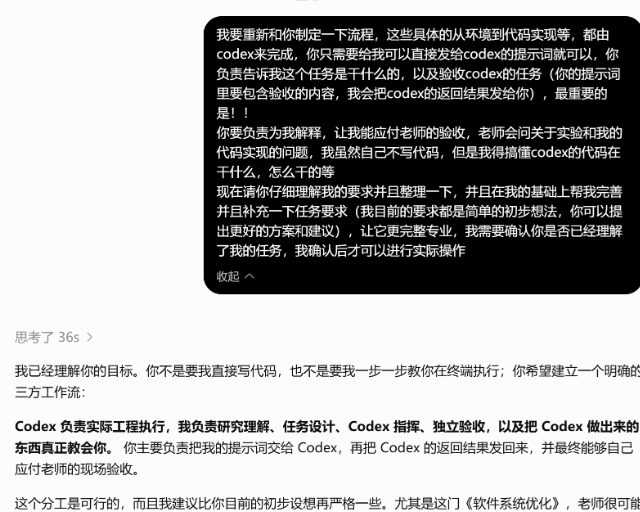
\includegraphics[width=136.500mm]{assets/crops/W01_01_01.png}};
\node[anchor=north west,inner sep=0,text width=136.50mm,align=left] at (14.00,167.23) {\color{Muted}\fontsize{7.2}{9.5}\selectfont  同一回答的后半段};
\node[anchor=north west,inner sep=0] at (14.000,171.428) {
\includegraphics[width=136.500mm]{assets/crops/W01_01_02.png}};
\node[anchor=north west,inner sep=0,text width=36.40mm,align=left] at (159.60,54.63) {\color{Blue}\fontsize{9.5}{13}\selectfont \bfseries 先明确执行分工};
\node[anchor=north west,inner sep=0,text width=36.40mm,align=left] at (159.60,63.28) {\color{Ink}\fontsize{8.7}{12.8}\selectfont  我把环境和代码实现交给 Codex，同时请 GPT 解释任务、设计工作，并在结果返回后帮我检查。};
\draw[draw=Blue,line width=.66pt,rounded corners=1mm,-{Stealth[length=1.8mm,width=1.35mm]}] (157.400,58.128) -- (153.200,58.128) -- (153.200,143.686) -- (149.860,143.686);
\node[anchor=north west,inner sep=0,text width=36.40mm,align=left] at (159.60,100.37) {\color{Violet}\fontsize{9.5}{13}\selectfont \bfseries 理解贯穿整个过程};
\node[anchor=north west,inner sep=0,text width=36.40mm,align=left] at (159.60,109.02) {\color{Ink}\fontsize{8.7}{12.8}\selectfont  我还要求把代码和实验原理讲到我能自己解释。后来，方法复盘和理解验收沿着这一要求继续展开。};
\draw[draw=Violet,line width=.66pt,rounded corners=1mm,-{Stealth[length=1.8mm,width=1.35mm]}] (157.400,103.872) -- (155.300,103.872) -- (155.300,228.374) -- (115.522,228.374);
\node[anchor=north west,inner sep=0,text width=36.40mm,align=left] at (159.60,146.12) {\color{Rose}\fontsize{8.9}{12.5}\selectfont \bfseries 我的回看};
\node[anchor=north west,inner sep=0,text width=36.40mm,align=left] at (159.60,153.12) {\color{Ink}\fontsize{8.5}{12.7}\selectfont  这段经验给了我一个可用的起点。进入新课程后，数据、参数和 AI 建议的判断又提出了新问题。};
\draw[Rule,line width=.35pt] (14,283)--(196,283);
\node[anchor=north west,inner sep=0,text width=170.00mm,align=left] at (14.00,287.00) {\color{Muted}\fontsize{6.7}{8.5}\selectfont  智慧城市与位置服务  /  实验一过程报告  /  Part I};
\node[anchor=north west,inner sep=0,text width=11.00mm,align=left] at (185.00,286.50) {\color{Muted}\fontsize{8}{9}\selectfont  03};
\PageEnd

\PageStart
\node[anchor=north west,inner sep=0,text width=182.00mm,align=left] at (14.00,11.00) {\color{Rose}\fontsize{7.8}{10}\selectfont \bfseries PART I · 工作流构建  /  协作方式的起点};
\node[anchor=north west,inner sep=0,text width=182.00mm,align=left] at (14.00,22.00) {\color{Ink}\fontsize{17.5}{22.5}\selectfont \bfseries 迁移之前，先让真实任务检验旧经验};
\node[anchor=north west,inner sep=0,text width=182.00mm,align=left] at (14.00,33.51) {\color{Ink}\fontsize{9.5}{14.6}\selectfont  进入智慧城市项目后，我先让 GPT 判断旧课程的做法哪些可以借用、哪些需要重新设计。随后我把第一次正式任务发给它，请它按老师材料检查这些做法是否合适。};
\node[anchor=north west,inner sep=0] at (14,8) {\hypertarget{W02}{}};
\node[anchor=north west,inner sep=0,text width=136.50mm,align=left] at (14.00,48.63) {\color{Muted}\fontsize{7.2}{9.5}\selectfont  迁移请求与初步回应};
\node[anchor=north west,inner sep=0] at (14.000,52.828) {
\includegraphics[width=136.500mm]{assets/crops/W02_01_01.png}};
\node[anchor=north west,inner sep=0,text width=136.50mm,align=left] at (14.00,132.90) {\color{Muted}\fontsize{7.2}{9.5}\selectfont  我补充第一次真实任务};
\node[anchor=north west,inner sep=0] at (14.000,137.102) {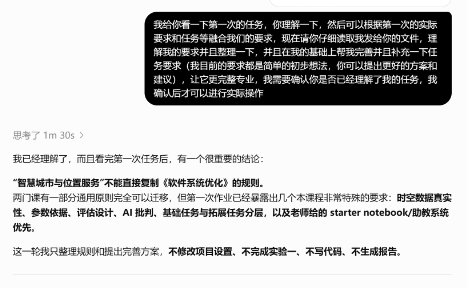
\includegraphics[width=136.500mm]{assets/crops/W02_01_02.png}};
\node[anchor=north west,inner sep=0,text width=136.50mm,align=left] at (14.00,226.48) {\color{Muted}\fontsize{7.2}{9.5}\selectfont  同一阶段：任务包的边界};
\node[anchor=north west,inner sep=0] at (14.000,230.682) {
\includegraphics[width=136.500mm]{assets/crops/W02_01_03.png}};
\node[anchor=north west,inner sep=0,text width=36.40mm,align=left] at (159.60,54.63) {\color{Blue}\fontsize{9.5}{13}\selectfont \bfseries 按新任务调整做法};
\node[anchor=north west,inner sep=0,text width=36.40mm,align=left] at (159.60,63.28) {\color{Ink}\fontsize{8.7}{12.8}\selectfont  时空数据、参数、评价和 AI 建议带来了新的判断问题。GPT据此补充了原有分工中缺少的研究环节。};
\draw[draw=Blue,line width=.66pt,rounded corners=1mm,-{Stealth[length=1.8mm,width=1.35mm]}] (157.400,58.128) -- (153.200,58.128) -- (153.200,110.279) -- (149.348,110.279);
\node[anchor=north west,inner sep=0,text width=36.40mm,align=left] at (159.60,100.37) {\color{Violet}\fontsize{9.5}{13}\selectfont \bfseries 分清材料的用途};
\node[anchor=north west,inner sep=0,text width=36.40mm,align=left] at (159.60,109.02) {\color{Ink}\fontsize{8.7}{12.8}\selectfont  老师材料用来确定任务，已有代码用来检查和复用，历史输出用作参考。本轮成果则需要通过实际处理和验证形成。};
\draw[draw=Violet,line width=.66pt,rounded corners=1mm,-{Stealth[length=1.8mm,width=1.35mm]}] (157.400,103.872) -- (155.300,103.872) -- (155.300,250.182) -- (114.701,250.182);
\draw[Rule,line width=.35pt] (14,283)--(196,283);
\node[anchor=north west,inner sep=0,text width=170.00mm,align=left] at (14.00,287.00) {\color{Muted}\fontsize{6.7}{8.5}\selectfont  智慧城市与位置服务  /  实验一过程报告  /  Part I};
\node[anchor=north west,inner sep=0,text width=11.00mm,align=left] at (185.00,286.50) {\color{Muted}\fontsize{8}{9}\selectfont  04};
\PageEnd

\PageStart
\node[anchor=north west,inner sep=0,text width=182.00mm,align=left] at (14.00,11.00) {\color{Rose}\fontsize{7.8}{10}\selectfont \bfseries PART I · 工作流构建  /  范围与研究判断};
\node[anchor=north west,inner sep=0,text width=182.00mm,align=left] at (14.00,22.00) {\color{Ink}\fontsize{17.5}{22.5}\selectfont \bfseries 老师的选做要做，额外扩展另作判断};
\node[anchor=north west,inner sep=0,text width=182.00mm,align=left] at (14.00,33.51) {\color{Ink}\fontsize{9.5}{14.6}\selectfont  我把两类“多做一点”分开：老师列出的选做、拓展和思考题也要完成；GPT 额外想到的内容先说明价值，再由我决定是否加入。这样既能覆盖课程任务，也能控制额外工作的范围。};
\node[anchor=north west,inner sep=0] at (14,8) {\hypertarget{W03}{}};
\node[anchor=north west,inner sep=0,text width=129.46mm,align=left] at (14.00,48.63) {\color{Muted}\fontsize{7.2}{9.5}\selectfont  我的原始补充：第1点};
\node[anchor=north west,inner sep=0] at (53.654,52.828) {
\includegraphics[width=89.805mm]{assets/crops/W03_01_01.png}};
\node[anchor=north west,inner sep=0,text width=129.46mm,align=left] at (14.00,76.11) {\color{Muted}\fontsize{7.2}{9.5}\selectfont  GPT把要求整理为任务层级};
\node[anchor=north west,inner sep=0] at (14.000,80.306) {
\includegraphics[width=129.460mm]{assets/crops/W03_01_02.png}};
\node[anchor=north west,inner sep=0,text width=129.46mm,align=left] at (14.00,139.91) {\color{Muted}\fontsize{7.2}{9.5}\selectfont  继续区分额外增强};
\node[anchor=north west,inner sep=0] at (14.000,144.108) {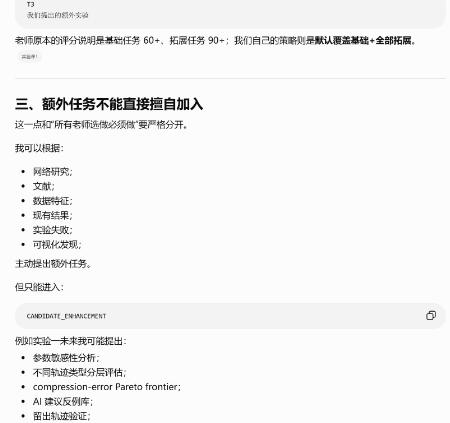
\includegraphics[width=129.460mm]{assets/crops/W03_01_03.png}};
\node[anchor=north west,inner sep=0,text width=36.40mm,align=left] at (159.60,54.63) {\color{Blue}\fontsize{9.5}{13}\selectfont \bfseries 两类要求一起保留};
\node[anchor=north west,inner sep=0,text width=36.40mm,align=left] at (159.60,63.28) {\color{Ink}\fontsize{8.7}{12.8}\selectfont  我希望完整完成老师的选做内容，同时保留对额外想法的选择。GPT随后把两者分别列入任务范围和候选增强。};
\draw[draw=Blue,line width=.66pt,rounded corners=1mm,-{Stealth[length=1.8mm,width=1.35mm]}] (157.400,58.128) -- (153.200,58.128) -- (153.200,68.573) -- (101.473,68.573);
\node[anchor=north west,inner sep=0,text width=36.40mm,align=left] at (159.60,104.89) {\color{Violet}\fontsize{9.5}{13}\selectfont \bfseries GPT整理任务层级};
\node[anchor=north west,inner sep=0,text width=36.40mm,align=left] at (159.60,113.54) {\color{Ink}\fontsize{8.7}{12.8}\selectfont  我先用自己的话提出要求，GPT随后用 T1、T2、T3 整理成分类，便于我们继续检查任务归属。};
\draw[draw=Violet,line width=.66pt,rounded corners=1mm,-{Stealth[length=1.8mm,width=1.35mm]}] (157.400,108.388) -- (155.300,108.388) -- (155.300,155.616) -- (134.254,155.616);
\draw[Rule,line width=.35pt] (14,283)--(196,283);
\node[anchor=north west,inner sep=0,text width=170.00mm,align=left] at (14.00,287.00) {\color{Muted}\fontsize{6.7}{8.5}\selectfont  智慧城市与位置服务  /  实验一过程报告  /  Part I};
\node[anchor=north west,inner sep=0,text width=11.00mm,align=left] at (185.00,286.50) {\color{Muted}\fontsize{8}{9}\selectfont  05};
\PageEnd

\PageStart
\node[anchor=north west,inner sep=0,text width=182.00mm,align=left] at (14.00,11.00) {\color{Rose}\fontsize{7.8}{10}\selectfont \bfseries PART I · 工作流构建  /  范围与研究判断};
\node[anchor=north west,inner sep=0,text width=182.00mm,align=left] at (14.00,22.00) {\color{Ink}\fontsize{17.5}{22.5}\selectfont \bfseries 查阅资料时，我还要知道它支持什么};
\node[anchor=north west,inner sep=0,text width=182.00mm,align=left] at (14.00,33.51) {\color{Ink}\fontsize{9.5}{14.6}\selectfont  任务范围理清后，我又要求在需要时主动检索并审核来源。我希望每个重要判断都有可回查的依据：找到网页以后，还要追到原文，看它究竟支持哪条结论。};
\node[anchor=north west,inner sep=0] at (14,8) {\hypertarget{W04}{}};
\node[anchor=north west,inner sep=0,text width=135.00mm,align=left] at (14.00,48.63) {\color{Muted}\fontsize{7.2}{9.5}\selectfont  我的原始补充：网络研究};
\node[anchor=north west,inner sep=0] at (55.351,52.828) {
\includegraphics[width=93.647mm]{assets/crops/W04_01_01.png}};
\node[anchor=north west,inner sep=0,text width=135.00mm,align=left] at (14.00,71.10) {\color{Muted}\fontsize{7.2}{9.5}\selectfont  GPT补充Source Audit与来源顺序};
\node[anchor=north west,inner sep=0] at (14.000,75.302) {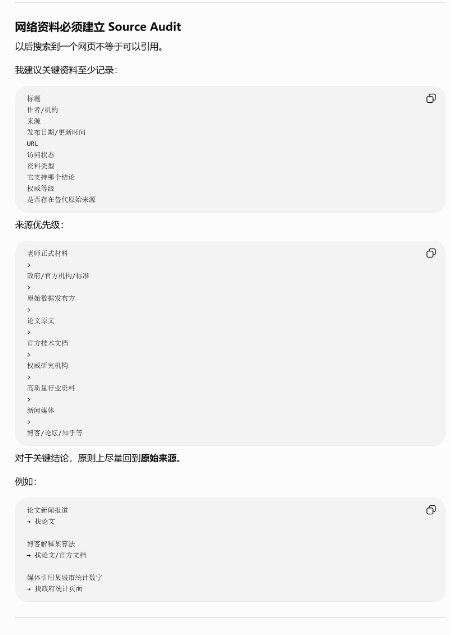
\includegraphics[width=134.998mm]{assets/crops/W04_01_02.png}};
\node[anchor=north west,inner sep=0,text width=36.40mm,align=left] at (159.60,54.63) {\color{Blue}\fontsize{9.5}{13}\selectfont \bfseries 关键判断要能回查};
\node[anchor=north west,inner sep=0,text width=36.40mm,align=left] at (159.60,63.28) {\color{Ink}\fontsize{8.7}{12.8}\selectfont  我要求链接真实可访问，关键内容经过核对。文献的标题之外，还要留下与当前问题有关的依据。};
\draw[draw=Blue,line width=.66pt,rounded corners=1mm,-{Stealth[length=1.8mm,width=1.35mm]}] (157.400,58.128) -- (153.200,58.128) -- (153.200,63.470) -- (98.830,63.470);
\node[anchor=north west,inner sep=0,text width=36.40mm,align=left] at (159.60,100.37) {\color{Violet}\fontsize{9.5}{13}\selectfont \bfseries 把来源与判断对应起来};
\node[anchor=north west,inner sep=0,text width=36.40mm,align=left] at (159.60,109.02) {\color{Ink}\fontsize{8.7}{12.8}\selectfont  GPT将作者、时间、来源类型和支持关系整理进 Source Audit；老师材料负责确定任务，外部资料帮助我们判断方案。};
\draw[draw=Violet,line width=.66pt,rounded corners=1mm,-{Stealth[length=1.8mm,width=1.35mm]}] (157.400,103.872) -- (155.300,103.872) -- (155.300,212.551) -- (69.199,212.551);
\node[anchor=north west,inner sep=0,text width=36.40mm,align=left] at (159.60,150.63) {\color{Rose}\fontsize{8.9}{12.5}\selectfont \bfseries 我的回看};
\node[anchor=north west,inner sep=0,text width=36.40mm,align=left] at (159.60,157.63) {\color{Ink}\fontsize{8.5}{12.7}\selectfont  这条要求后来直接影响实验一的检索：每篇论文都要说明怎样帮助处理轨迹问题。};
\draw[Rule,line width=.35pt] (14,283)--(196,283);
\node[anchor=north west,inner sep=0,text width=170.00mm,align=left] at (14.00,287.00) {\color{Muted}\fontsize{6.7}{8.5}\selectfont  智慧城市与位置服务  /  实验一过程报告  /  Part I};
\node[anchor=north west,inner sep=0,text width=11.00mm,align=left] at (185.00,286.50) {\color{Muted}\fontsize{8}{9}\selectfont  06};
\PageEnd

\PageStart
\node[anchor=north west,inner sep=0,text width=182.00mm,align=left] at (14.00,11.00) {\color{Rose}\fontsize{7.8}{10}\selectfont \bfseries PART I · 工作流构建  /  范围与研究判断};
\node[anchor=north west,inner sep=0,text width=182.00mm,align=left] at (14.00,22.00) {\color{Ink}\fontsize{17.5}{22.5}\selectfont \bfseries 不确定时，先比较候选，再让实验说话};
\node[anchor=north west,inner sep=0,text width=182.00mm,align=left] at (14.00,33.51) {\color{Ink}\fontsize{9.5}{14.6}\selectfont  面对有分歧的问题，我希望 GPT 先给少量有根据的候选，讲清各自的依据和问题。讨论后仍无法决定，就固定比较条件，让实验结果帮助我们取舍。};
\node[anchor=north west,inner sep=0] at (14,8) {\hypertarget{W05}{}};
\node[anchor=north west,inner sep=0,text width=136.50mm,align=left] at (14.00,48.63) {\color{Muted}\fontsize{7.2}{9.5}\selectfont  我的原始补充：第3点};
\node[anchor=north west,inner sep=0] at (55.811,52.828) {
\includegraphics[width=94.689mm]{assets/crops/W05_01_01.png}};
\node[anchor=north west,inner sep=0,text width=136.50mm,align=left] at (14.00,83.55) {\color{Muted}\fontsize{7.2}{9.5}\selectfont  GPT区分候选与未决问题};
\node[anchor=north west,inner sep=0] at (14.000,87.745) {
\includegraphics[width=136.500mm]{assets/crops/W05_01_02.png}};
\node[anchor=north west,inner sep=0,text width=136.50mm,align=left] at (14.00,145.58) {\color{Muted}\fontsize{7.2}{9.5}\selectfont  同一回答：讨论不足时进入比较};
\node[anchor=north west,inner sep=0] at (14.000,149.781) {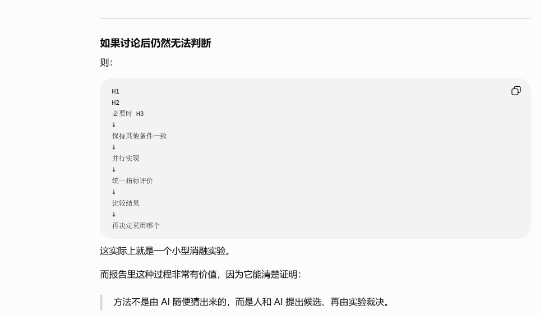
\includegraphics[width=136.500mm]{assets/crops/W05_01_03.png}};
\node[anchor=north west,inner sep=0,text width=36.40mm,align=left] at (159.60,54.63) {\color{Blue}\fontsize{9.5}{13}\selectfont \bfseries 把不确定性摊开讨论};
\node[anchor=north west,inner sep=0,text width=36.40mm,align=left] at (159.60,63.28) {\color{Ink}\fontsize{8.7}{12.8}\selectfont  我提出先看两三种合理方案，再判断是否需要实验。这样可以一起检查假设，也能看清每个候选的代价。};
\draw[draw=Blue,line width=.66pt,rounded corners=1mm,-{Stealth[length=1.8mm,width=1.35mm]}] (157.400,58.128) -- (153.200,58.128) -- (153.200,75.732) -- (94.240,75.732);
\node[anchor=north west,inner sep=0,text width=36.40mm,align=left] at (159.60,100.37) {\color{Violet}\fontsize{9.5}{13}\selectfont \bfseries 为下一步确定依据};
\node[anchor=north west,inner sep=0,text width=36.40mm,align=left] at (159.60,109.02) {\color{Ink}\fontsize{8.7}{12.8}\selectfont  GPT后来用 CANDIDATE、UNRESOLVED 记录不同情况：有合理候选时继续比较，讨论不足时转入公平实验。};
\draw[draw=Violet,line width=.66pt,rounded corners=1mm,-{Stealth[length=1.8mm,width=1.35mm]}] (157.400,103.872) -- (155.300,103.872) -- (155.300,225.586) -- (112.471,225.586);
\draw[Rule,line width=.35pt] (14,283)--(196,283);
\node[anchor=north west,inner sep=0,text width=170.00mm,align=left] at (14.00,287.00) {\color{Muted}\fontsize{6.7}{8.5}\selectfont  智慧城市与位置服务  /  实验一过程报告  /  Part I};
\node[anchor=north west,inner sep=0,text width=11.00mm,align=left] at (185.00,286.50) {\color{Muted}\fontsize{8}{9}\selectfont  07};
\PageEnd

\PageStart
\node[anchor=north west,inner sep=0,text width=182.00mm,align=left] at (14.00,11.00) {\color{Rose}\fontsize{7.8}{10}\selectfont \bfseries PART I · 工作流构建  /  范围与研究判断};
\node[anchor=north west,inner sep=0,text width=182.00mm,align=left] at (14.00,22.00) {\color{Ink}\fontsize{17.5}{22.5}\selectfont \bfseries 我的参与体现在质疑、修改与选择中};
\node[anchor=north west,inner sep=0,text width=182.00mm,align=left] at (14.00,33.51) {\color{Ink}\fontsize{9.5}{14.6}\selectfont  我明确要求参与讨论和判断。重要假设、方法或结论有问题时，我可以质疑、修改、否决，也可以要求再验证；普通工具操作则按已经确定的规则继续执行。};
\node[anchor=north west,inner sep=0] at (14,8) {\hypertarget{W06}{}};
\node[anchor=north west,inner sep=0,text width=130.33mm,align=left] at (14.00,48.63) {\color{Muted}\fontsize{7.2}{9.5}\selectfont  我的原始补充：人的参与};
\node[anchor=north west,inner sep=0] at (53.920,52.828) {
\includegraphics[width=90.407mm]{assets/crops/W06_01_01.png}};
\node[anchor=north west,inner sep=0,text width=130.33mm,align=left] at (14.00,77.69) {\color{Muted}\fontsize{7.2}{9.5}\selectfont  GPT明确判断与执行的分工};
\node[anchor=north west,inner sep=0] at (14.000,81.895) {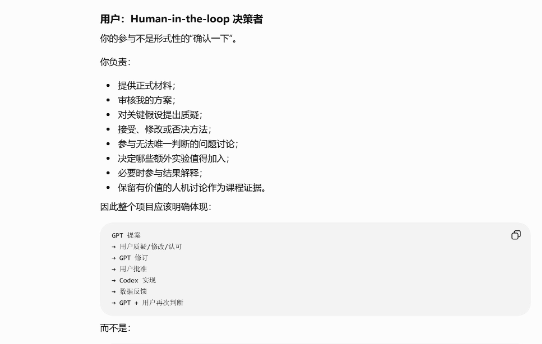
\includegraphics[width=130.326mm]{assets/crops/W06_01_02.png}};
\node[anchor=north west,inner sep=0,text width=130.33mm,align=left] at (14.00,169.81) {\color{Muted}\fontsize{7.2}{9.5}\selectfont  AI建议还需要证据};
\node[anchor=north west,inner sep=0] at (14.000,174.011) {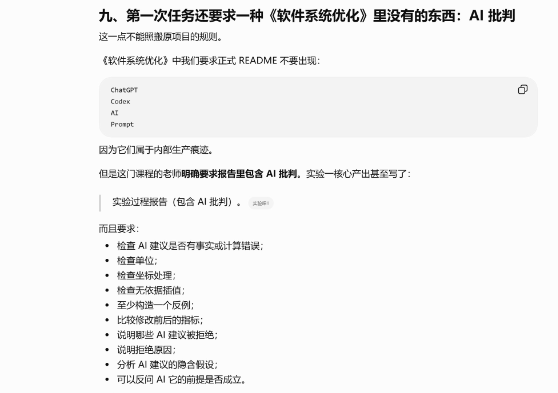
\includegraphics[width=130.326mm]{assets/crops/W06_01_03.png}};
\node[anchor=north west,inner sep=0,text width=36.40mm,align=left] at (159.60,54.63) {\color{Blue}\fontsize{9.5}{13}\selectfont \bfseries 我的判断能改变方案};
\node[anchor=north west,inner sep=0,text width=36.40mm,align=left] at (159.60,63.28) {\color{Ink}\fontsize{8.7}{12.8}\selectfont  我希望在关键问题出现时进入讨论，提出自己的看法，再和 GPT 一起决定怎样继续。};
\draw[draw=Blue,line width=.66pt,rounded corners=1mm,-{Stealth[length=1.8mm,width=1.35mm]}] (157.400,58.128) -- (153.200,58.128) -- (153.200,66.477) -- (140.511,66.477);
\node[anchor=north west,inner sep=0,text width=36.40mm,align=left] at (159.60,100.37) {\color{Violet}\fontsize{9.5}{13}\selectfont \bfseries 把质疑落到具体依据};
\node[anchor=north west,inner sep=0,text width=36.40mm,align=left] at (159.60,109.02) {\color{Ink}\fontsize{8.7}{12.8}\selectfont  反例、单位、坐标和前后指标，让我们能够检验分歧。GPT把这些内容补进了 AI 建议的核查过程。};
\draw[draw=Violet,line width=.66pt,rounded corners=1mm,-{Stealth[length=1.8mm,width=1.35mm]}] (157.400,103.872) -- (155.300,103.872) -- (155.300,262.530) -- (71.923,262.530);
\draw[Rule,line width=.35pt] (14,283)--(196,283);
\node[anchor=north west,inner sep=0,text width=170.00mm,align=left] at (14.00,287.00) {\color{Muted}\fontsize{6.7}{8.5}\selectfont  智慧城市与位置服务  /  实验一过程报告  /  Part I};
\node[anchor=north west,inner sep=0,text width=11.00mm,align=left] at (185.00,286.50) {\color{Muted}\fontsize{8}{9}\selectfont  08};
\PageEnd

\PageStart
\node[anchor=north west,inner sep=0,text width=182.00mm,align=left] at (14.00,11.00) {\color{Rose}\fontsize{7.8}{10}\selectfont \bfseries PART I · 工作流构建  /  报告与视觉表达};
\node[anchor=north west,inner sep=0,text width=182.00mm,align=left] at (14.00,22.00) {\color{Ink}\fontsize{17.5}{22.5}\selectfont \bfseries 分别记录最终结果与方案形成过程};
\node[anchor=north west,inner sep=0,text width=182.00mm,align=left] at (14.00,33.51) {\color{Ink}\fontsize{9.5}{14.6}\selectfont  随着讨论变多，我发现只保留最后结果会丢掉方案形成的过程。因此我要求两份报告各自回答问题：Experiment Report解释最终方法、实验与结论，Process Report记录我怎样讨论、判断和验证。};
\node[anchor=north west,inner sep=0] at (14,8) {\hypertarget{W07}{}};
\node[anchor=north west,inner sep=0,text width=136.50mm,align=left] at (14.00,48.63) {\color{Muted}\fontsize{7.2}{9.5}\selectfont  我提出两类文档，GPT回应};
\node[anchor=north west,inner sep=0] at (14.000,52.828) {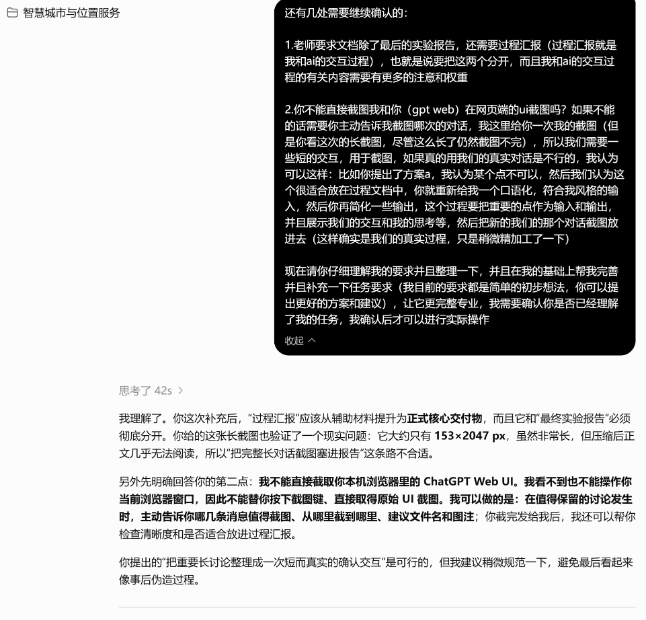
\includegraphics[width=136.500mm]{assets/crops/W07_01_01.png}};
\node[anchor=north west,inner sep=0,text width=136.50mm,align=left] at (14.00,189.03) {\color{Muted}\fontsize{7.2}{9.5}\selectfont  同一轮：过程报告的定位};
\node[anchor=north west,inner sep=0] at (14.000,193.234) {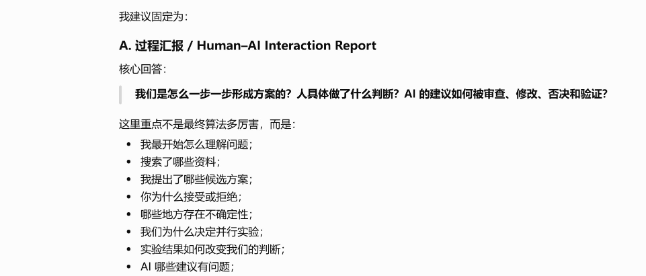
\includegraphics[width=136.500mm]{assets/crops/W07_01_02.png}};
\node[anchor=north west,inner sep=0,text width=36.40mm,align=left] at (159.60,54.63) {\color{Blue}\fontsize{9.5}{13}\selectfont \bfseries 两份报告各有重点};
\node[anchor=north west,inner sep=0,text width=36.40mm,align=left] at (159.60,63.28) {\color{Ink}\fontsize{8.7}{12.8}\selectfont  实验报告帮助老师理解做法与结果；过程报告让老师看到这些做法怎样在互动和验证中形成。};
\draw[draw=Blue,line width=.66pt,rounded corners=1mm,-{Stealth[length=1.8mm,width=1.35mm]}] (157.400,58.128) -- (153.200,58.128) -- (153.200,62.231) -- (145.217,62.231);
\node[anchor=north west,inner sep=0,text width=36.40mm,align=left] at (159.60,100.37) {\color{Violet}\fontsize{9.5}{13}\selectfont \bfseries 保留改变方案的经过};
\node[anchor=north west,inner sep=0,text width=36.40mm,align=left] at (159.60,109.02) {\color{Ink}\fontsize{8.7}{12.8}\selectfont  我为什么改方案、什么证据改变了判断，是这份过程报告需要讲清的内容。};
\draw[draw=Violet,line width=.66pt,rounded corners=1mm,-{Stealth[length=1.8mm,width=1.35mm]}] (157.400,103.872) -- (155.300,103.872) -- (155.300,219.436) -- (77.179,219.436);
\node[anchor=north west,inner sep=0,text width=36.40mm,align=left] at (159.60,141.60) {\color{Rose}\fontsize{8.9}{12.5}\selectfont \bfseries 我的回看};
\node[anchor=north west,inner sep=0,text width=36.40mm,align=left] at (159.60,148.60) {\color{Ink}\fontsize{8.5}{12.7}\selectfont  同一事实可以进入两份报告：一处解释技术理由，另一处说明这个理由怎样在讨论中形成。};
\draw[Rule,line width=.35pt] (14,283)--(196,283);
\node[anchor=north west,inner sep=0,text width=170.00mm,align=left] at (14.00,287.00) {\color{Muted}\fontsize{6.7}{8.5}\selectfont  智慧城市与位置服务  /  实验一过程报告  /  Part I};
\node[anchor=north west,inner sep=0,text width=11.00mm,align=left] at (185.00,286.50) {\color{Muted}\fontsize{8}{9}\selectfont  09};
\PageEnd

\PageStart
\node[anchor=north west,inner sep=0,text width=182.00mm,align=left] at (14.00,11.00) {\color{Rose}\fontsize{7.8}{10}\selectfont \bfseries PART I · 工作流构建  /  报告与视觉表达};
\node[anchor=north west,inner sep=0,text width=182.00mm,align=left] at (14.00,22.00) {\color{Ink}\fontsize{17.5}{22.5}\selectfont \bfseries 围绕关键决策整理分散的对话};
\node[anchor=north west,inner sep=0,text width=182.00mm,align=left] at (14.00,33.51) {\color{Ink}\fontsize{9.5}{14.6}\selectfont  一次决定常常跨越几轮讨论，中间还会有后补说明。我希望把相关内容放到一起，让读者顺着问题、回应、验证和取舍，理解这次决定怎样形成。};
\node[anchor=north west,inner sep=0] at (14,8) {\hypertarget{W08}{}};
\node[anchor=north west,inner sep=0,text width=133.44mm,align=left] at (14.00,48.63) {\color{Muted}\fontsize{7.2}{9.5}\selectfont  回引前页要求：保存过程记录};
\node[anchor=north west,inner sep=0] at (67.294,52.828) {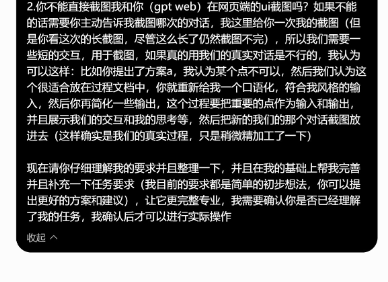
\includegraphics[width=80.147mm]{assets/crops/W08_01_01.png}};
\node[anchor=north west,inner sep=0,text width=133.44mm,align=left] at (14.00,116.28) {\color{Muted}\fontsize{7.2}{9.5}\selectfont  GPT建议按决策事件组织};
\node[anchor=north west,inner sep=0] at (14.000,120.480) {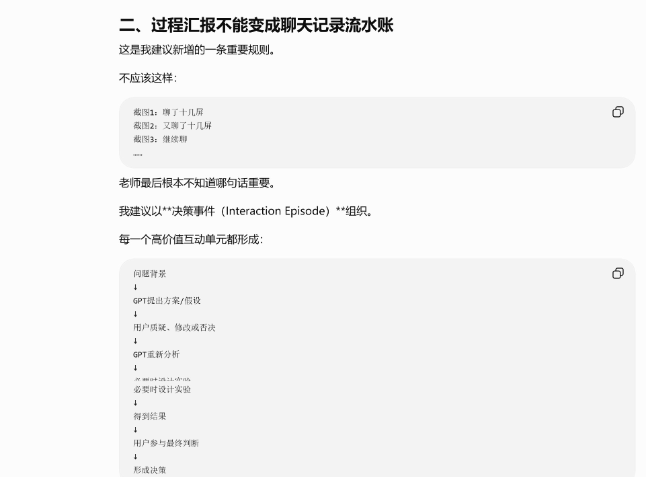
\includegraphics[width=133.441mm]{assets/crops/W08_01_02.png}};
\node[anchor=north west,inner sep=0,text width=133.44mm,align=left] at (14.00,224.21) {\color{Muted}\fontsize{7.2}{9.5}\selectfont  自然讨论结束后的简短确认};
\node[anchor=north west,inner sep=0] at (14.000,228.412) {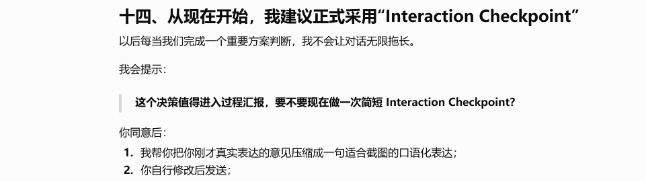
\includegraphics[width=133.441mm]{assets/crops/W08_01_03.png}};
\node[anchor=north west,inner sep=0,text width=36.40mm,align=left] at (159.60,54.63) {\color{Blue}\fontsize{9.5}{13}\selectfont \bfseries 把相关讨论归在一起};
\node[anchor=north west,inner sep=0,text width=36.40mm,align=left] at (159.60,63.28) {\color{Ink}\fontsize{8.7}{12.8}\selectfont  我提出要保存有意义的互动，GPT随后建议按决策事件组织。一个问题分散在几轮里，也可以沿着它的变化一起阅读。};
\draw[draw=Blue,line width=.66pt,rounded corners=1mm,-{Stealth[length=1.8mm,width=1.35mm]}] (157.400,58.128) -- (153.200,58.128) -- (153.200,77.410) -- (142.484,77.410);
\node[anchor=north west,inner sep=0,text width=36.40mm,align=left] at (159.60,104.89) {\color{Violet}\fontsize{9.5}{13}\selectfont \bfseries 讨论清楚后作简短确认};
\node[anchor=north west,inner sep=0,text width=36.40mm,align=left] at (159.60,113.54) {\color{Ink}\fontsize{8.7}{12.8}\selectfont  关键问题形成结论后，再用简短确认记录选择和理由。这样既保留真实推进过程，也方便后续回查。};
\draw[draw=Violet,line width=.66pt,rounded corners=1mm,-{Stealth[length=1.8mm,width=1.35mm]}] (157.400,108.388) -- (155.300,108.388) -- (155.300,263.424) -- (62.336,263.424);
\draw[Rule,line width=.35pt] (14,283)--(196,283);
\node[anchor=north west,inner sep=0,text width=170.00mm,align=left] at (14.00,287.00) {\color{Muted}\fontsize{6.7}{8.5}\selectfont  智慧城市与位置服务  /  实验一过程报告  /  Part I};
\node[anchor=north west,inner sep=0,text width=11.00mm,align=left] at (185.00,286.50) {\color{Muted}\fontsize{8}{9}\selectfont  10};
\PageEnd

\PageStart
\node[anchor=north west,inner sep=0,text width=182.00mm,align=left] at (14.00,11.00) {\color{Rose}\fontsize{7.8}{10}\selectfont \bfseries PART I · 工作流构建  /  报告与视觉表达};
\node[anchor=north west,inner sep=0,text width=182.00mm,align=left] at (14.00,22.00) {\color{Ink}\fontsize{17.5}{22.5}\selectfont \bfseries 让图帮助发现和解释轨迹问题};
\node[anchor=north west,inner sep=0,text width=182.00mm,align=left] at (14.00,33.51) {\color{Ink}\fontsize{9.5}{14.6}\selectfont  我希望智慧城市报告有更丰富的可视化，重点是让图与数据和研究问题对应。我关心图能否解释异常、参数变化和结果取舍，也希望图能帮助我们发现下一步需要研究的问题。};
\node[anchor=north west,inner sep=0] at (14,8) {\hypertarget{W09}{}};
\node[anchor=north west,inner sep=0,text width=129.90mm,align=left] at (14.00,48.63) {\color{Muted}\fontsize{7.2}{9.5}\selectfont  我提出可视化要求};
\node[anchor=north west,inner sep=0] at (14.000,52.828) {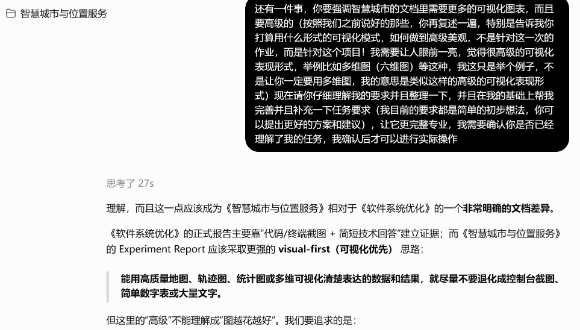
\includegraphics[width=129.896mm]{assets/crops/W09_01_01.png}};
\node[anchor=north west,inner sep=0,text width=129.90mm,align=left] at (14.00,131.93) {\color{Muted}\fontsize{7.2}{9.5}\selectfont  GPT把图的研究职责展开};
\node[anchor=north west,inner sep=0] at (14.000,136.134) {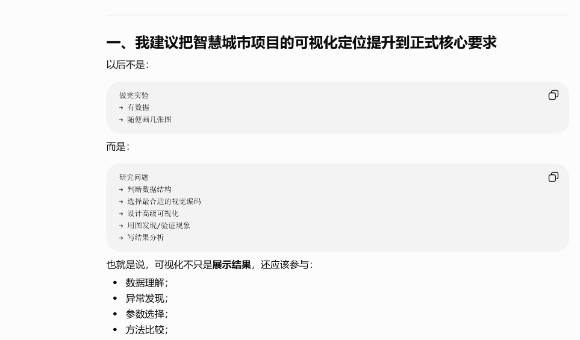
\includegraphics[width=129.896mm]{assets/crops/W09_01_02.png}};
\node[anchor=north west,inner sep=0,text width=129.90mm,align=left] at (14.00,217.48) {\color{Muted}\fontsize{7.2}{9.5}\selectfont  同一阶段：复杂度服从可读性};
\node[anchor=north west,inner sep=0] at (14.000,221.680) {
\includegraphics[width=129.896mm]{assets/crops/W09_01_03.png}};
\node[anchor=north west,inner sep=0,text width=36.40mm,align=left] at (159.60,54.63) {\color{Blue}\fontsize{9.5}{13}\selectfont \bfseries 图也参与研究};
\node[anchor=north west,inner sep=0,text width=36.40mm,align=left] at (159.60,63.28) {\color{Ink}\fontsize{8.7}{12.8}\selectfont  我希望图既展示结果，也帮助理解数据、发现问题和比较方案。GPT据此展开了不同图型的研究用途。};
\draw[draw=Blue,line width=.66pt,rounded corners=1mm,-{Stealth[length=1.8mm,width=1.35mm]}] (157.400,58.128) -- (153.200,58.128) -- (153.200,118.336) -- (64.167,118.336);
\node[anchor=north west,inner sep=0,text width=36.40mm,align=left] at (159.60,100.37) {\color{Violet}\fontsize{9.5}{13}\selectfont \bfseries 可读性优先};
\node[anchor=north west,inner sep=0,text width=36.40mm,align=left] at (159.60,109.02) {\color{Ink}\fontsize{8.7}{12.8}\selectfont  图型和复杂度都服从要解释的问题。技术图使用真实数据或明确结构，读者应能直接看清关键关系。};
\draw[draw=Violet,line width=.66pt,rounded corners=1mm,-{Stealth[length=1.8mm,width=1.35mm]}] (157.400,103.872) -- (155.300,103.872) -- (155.300,245.084) -- (96.865,245.084);
\draw[Rule,line width=.35pt] (14,283)--(196,283);
\node[anchor=north west,inner sep=0,text width=170.00mm,align=left] at (14.00,287.00) {\color{Muted}\fontsize{6.7}{8.5}\selectfont  智慧城市与位置服务  /  实验一过程报告  /  Part I};
\node[anchor=north west,inner sep=0,text width=11.00mm,align=left] at (185.00,286.50) {\color{Muted}\fontsize{8}{9}\selectfont  11};
\PageEnd

\PageStart
\node[anchor=north west,inner sep=0,text width=182.00mm,align=left] at (14.00,11.00) {\color{Rose}\fontsize{7.8}{10}\selectfont \bfseries PART I · 工作流构建  /  报告与视觉表达};
\node[anchor=north west,inner sep=0,text width=182.00mm,align=left] at (14.00,22.00) {\color{Ink}\fontsize{17.5}{22.5}\selectfont \bfseries 给关键互动足够的阅读空间};
\node[anchor=north west,inner sep=0,text width=182.00mm,align=left] at (14.00,33.51) {\color{Ink}\fontsize{9.5}{14.6}\selectfont  我希望关键上下文能够完整保留，因此提出按内容安排篇幅。原始截图先保存下来，正式页面再选择与判断相关的窗口；一般过程简要呈现，核心决策则展开说明。};
\node[anchor=north west,inner sep=0] at (14,8) {\hypertarget{W10}{}};
\node[anchor=north west,inner sep=0,text width=136.50mm,align=left] at (14.00,48.63) {\color{Muted}\fontsize{7.2}{9.5}\selectfont  我对证据页面的补充};
\node[anchor=north west,inner sep=0] at (56.525,52.828) {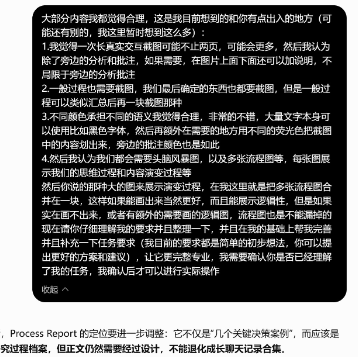
\includegraphics[width=93.975mm]{assets/crops/W10_01_01.png}};
\node[anchor=north west,inner sep=0,text width=136.50mm,align=left] at (14.00,151.74) {\color{Muted}\fontsize{7.2}{9.5}\selectfont  GPT改为按实际内容分页};
\node[anchor=north west,inner sep=0] at (14.000,155.941) {
\includegraphics[width=136.500mm]{assets/crops/W10_01_02.png}};
\node[anchor=north west,inner sep=0,text width=36.40mm,align=left] at (159.60,54.63) {\color{Blue}\fontsize{9.5}{13}\selectfont \bfseries 证据内容决定篇幅};
\node[anchor=north west,inner sep=0,text width=36.40mm,align=left] at (159.60,63.28) {\color{Ink}\fontsize{8.7}{12.8}\selectfont  我要求关键互动可以跨必要页数，并保留最后的确认。GPT随后把分页依据改为实际内容和阅读需要。};
\draw[draw=Blue,line width=.66pt,rounded corners=1mm,-{Stealth[length=1.8mm,width=1.35mm]}] (157.400,58.128) -- (153.200,58.128) -- (153.200,68.578) -- (148.663,68.578);
\node[anchor=north west,inner sep=0,text width=36.40mm,align=left] at (159.60,100.37) {\color{Violet}\fontsize{9.5}{13}\selectfont \bfseries 先保存，再组织阅读};
\node[anchor=north west,inner sep=0,text width=36.40mm,align=left] at (159.60,109.02) {\color{Ink}\fontsize{8.7}{12.8}\selectfont  原始发言与回应先保存完整，再安排节选、页序和侧注。这样后续修改版式时仍有可靠的原件可用。};
\draw[draw=Violet,line width=.66pt,rounded corners=1mm,-{Stealth[length=1.8mm,width=1.35mm]}] (157.400,103.872) -- (155.300,103.872) -- (155.300,197.594) -- (148.530,197.594);
\draw[Rule,line width=.35pt] (14,283)--(196,283);
\node[anchor=north west,inner sep=0,text width=170.00mm,align=left] at (14.00,287.00) {\color{Muted}\fontsize{6.7}{8.5}\selectfont  智慧城市与位置服务  /  实验一过程报告  /  Part I};
\node[anchor=north west,inner sep=0,text width=11.00mm,align=left] at (185.00,286.50) {\color{Muted}\fontsize{8}{9}\selectfont  12};
\PageEnd

\PageStart
\node[anchor=north west,inner sep=0,text width=182.00mm,align=left] at (14.00,11.00) {\color{Rose}\fontsize{7.8}{10}\selectfont \bfseries PART I · 工作流构建  /  报告与视觉表达};
\node[anchor=north west,inner sep=0,text width=182.00mm,align=left] at (14.00,22.00) {\color{Ink}\fontsize{17.5}{22.5}\selectfont \bfseries 用LaTeX建立两份报告的共同视觉基础};
\node[anchor=north west,inner sep=0,text width=182.00mm,align=left] at (14.00,33.51) {\color{Ink}\fontsize{9.5}{14.6}\selectfont  我提出统一使用 LaTeX，让字体、图注、颜色和引用有稳定基础。Experiment 与 Process 分别围绕结果和过程组织内容，在共同视觉体系下保留各自的阅读方式。};
\node[anchor=north west,inner sep=0] at (14,8) {\hypertarget{W11}{}};
\node[anchor=north west,inner sep=0,text width=132.07mm,align=left] at (14.00,48.63) {\color{Muted}\fontsize{7.2}{9.5}\selectfont  我的LaTeX与两份报告要求};
\node[anchor=north west,inner sep=0] at (57.556,52.828) {
\includegraphics[width=88.517mm]{assets/crops/W11_01_01.png}};
\node[anchor=north west,inner sep=0,text width=132.07mm,align=left] at (14.00,158.91) {\color{Muted}\fontsize{7.2}{9.5}\selectfont  GPT区分共享系统与报告布局};
\node[anchor=north west,inner sep=0] at (14.000,163.110) {
\includegraphics[width=132.073mm]{assets/crops/W11_01_02.png}};
\node[anchor=north west,inner sep=0,text width=36.40mm,align=left] at (159.60,54.63) {\color{Blue}\fontsize{9.5}{13}\selectfont \bfseries 共享视觉，分别叙述};
\node[anchor=north west,inner sep=0,text width=36.40mm,align=left] at (159.60,63.28) {\color{Ink}\fontsize{8.7}{12.8}\selectfont  两份报告沿用相同的视觉身份；实验方法与研究决策，则分别按各自的内容组织。};
\draw[draw=Blue,line width=.66pt,rounded corners=1mm,-{Stealth[length=1.8mm,width=1.35mm]}] (157.400,58.128) -- (153.200,58.128) -- (153.200,105.657) -- (145.230,105.657);
\node[anchor=north west,inner sep=0,text width=36.40mm,align=left] at (159.60,100.37) {\color{Violet}\fontsize{9.5}{13}\selectfont \bfseries 保留可修改的生成源};
\node[anchor=north west,inner sep=0,text width=36.40mm,align=left] at (159.60,109.02) {\color{Ink}\fontsize{8.7}{12.8}\selectfont  LaTeX正文、图形与构建方式一起保存。后续修订可以回到这些源文件，继续维护已经确认的表达。};
\draw[draw=Violet,line width=.66pt,rounded corners=1mm,-{Stealth[length=1.8mm,width=1.35mm]}] (157.400,103.872) -- (155.300,103.872) -- (155.300,240.276) -- (50.802,240.276);
\draw[Rule,line width=.35pt] (14,283)--(196,283);
\node[anchor=north west,inner sep=0,text width=170.00mm,align=left] at (14.00,287.00) {\color{Muted}\fontsize{6.7}{8.5}\selectfont  智慧城市与位置服务  /  实验一过程报告  /  Part I};
\node[anchor=north west,inner sep=0,text width=11.00mm,align=left] at (185.00,286.50) {\color{Muted}\fontsize{8}{9}\selectfont  13};
\PageEnd

\PageStart
\node[anchor=north west,inner sep=0,text width=182.00mm,align=left] at (14.00,11.00) {\color{Rose}\fontsize{7.8}{10}\selectfont \bfseries PART I · 工作流构建  /  报告与视觉表达};
\node[anchor=north west,inner sep=0,text width=182.00mm,align=left] at (14.00,22.00) {\color{Ink}\fontsize{17.5}{22.5}\selectfont \bfseries 从实际页面调整配色与留白};
\node[anchor=north west,inner sep=0,text width=182.00mm,align=left] at (14.00,33.51) {\color{Ink}\fontsize{9.5}{14.6}\selectfont  看过实际页面后，我觉得大面积色块和卡片太多。于是我要求减少装饰，让正文保持中性，把颜色留给真正需要强调的判断和对应关系。};
\node[anchor=north west,inner sep=0] at (14,8) {\hypertarget{W12}{}};
\node[anchor=north west,inner sep=0,text width=136.50mm,align=left] at (14.00,48.63) {\color{Muted}\fontsize{7.2}{9.5}\selectfont  我对实际页面的反馈};
\node[anchor=north west,inner sep=0] at (54.444,52.828) {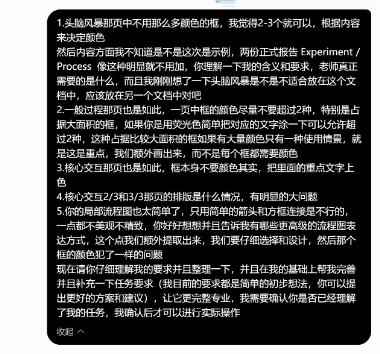
\includegraphics[width=96.056mm]{assets/crops/W12_01_01.png}};
\node[anchor=north west,inner sep=0,text width=136.50mm,align=left] at (14.00,147.51) {\color{Muted}\fontsize{7.2}{9.5}\selectfont  GPT补充克制的视觉规则};
\node[anchor=north west,inner sep=0] at (14.000,151.712) {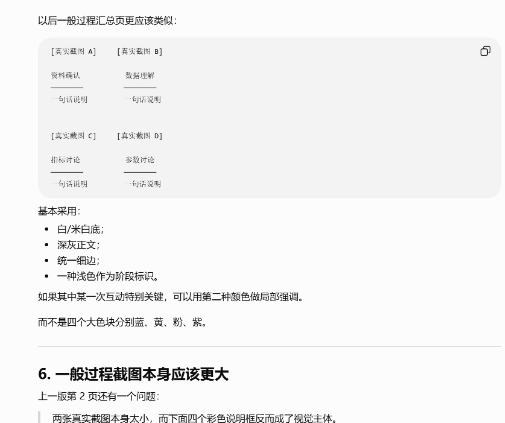
\includegraphics[width=136.500mm]{assets/crops/W12_01_02.png}};
\node[anchor=north west,inner sep=0,text width=36.40mm,align=left] at (159.60,54.63) {\color{Blue}\fontsize{9.5}{13}\selectfont \bfseries 根据阅读效果作修改};
\node[anchor=north west,inner sep=0,text width=36.40mm,align=left] at (159.60,63.28) {\color{Ink}\fontsize{8.7}{12.8}\selectfont  我的反馈来自实际页面：颜色和卡片抢走了注意力。GPT据此调整了大面积填色与强调方式。};
\draw[draw=Blue,line width=.66pt,rounded corners=1mm,-{Stealth[length=1.8mm,width=1.35mm]}] (157.400,58.128) -- (153.200,58.128) -- (153.200,80.507) -- (149.236,80.507);
\node[anchor=north west,inner sep=0,text width=36.40mm,align=left] at (159.60,100.37) {\color{Violet}\fontsize{9.5}{13}\selectfont \bfseries 让重点更容易找到};
\node[anchor=north west,inner sep=0,text width=36.40mm,align=left] at (159.60,109.02) {\color{Ink}\fontsize{8.7}{12.8}\selectfont  P2视觉体系继续保留，正文以中性色为主，颜色集中标明重要判断和对应关系。};
\draw[draw=Violet,line width=.66pt,rounded corners=1mm,-{Stealth[length=1.8mm,width=1.35mm]}] (157.400,103.872) -- (155.300,103.872) -- (155.300,226.178) -- (57.518,226.178);
\draw[Rule,line width=.35pt] (14,283)--(196,283);
\node[anchor=north west,inner sep=0,text width=170.00mm,align=left] at (14.00,287.00) {\color{Muted}\fontsize{6.7}{8.5}\selectfont  智慧城市与位置服务  /  实验一过程报告  /  Part I};
\node[anchor=north west,inner sep=0,text width=11.00mm,align=left] at (185.00,286.50) {\color{Muted}\fontsize{8}{9}\selectfont  14};
\PageEnd

\PageStart
\node[anchor=north west,inner sep=0,text width=182.00mm,align=left] at (14.00,11.00) {\color{Rose}\fontsize{7.8}{10}\selectfont \bfseries PART I · 工作流构建  /  报告与视觉表达};
\node[anchor=north west,inner sep=0,text width=182.00mm,align=left] at (14.00,22.00) {\color{Ink}\fontsize{17.5}{22.5}\selectfont \bfseries 让流程图呈现我的判断过程};
\node[anchor=north west,inner sep=0,text width=182.00mm,align=left] at (14.00,33.51) {\color{Ink}\fontsize{9.5}{14.6}\selectfont  我逐一看过候选图型，淘汰不合适的，要求把候选树改成横向。我还希望图里呈现我发现了什么、怎样理解问题、提出了什么修改，以及证据怎样支持最后的选择。};
\node[anchor=north west,inner sep=0] at (14,8) {\hypertarget{W13}{}};
\node[anchor=north west,inner sep=0,text width=136.50mm,align=left] at (14.00,48.63) {\color{Muted}\fontsize{7.2}{9.5}\selectfont  我的图型反馈与GPT回应};
\node[anchor=north west,inner sep=0] at (14.000,52.828) {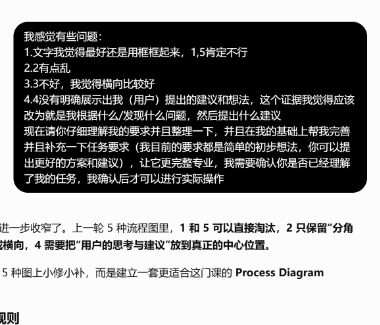
\includegraphics[width=99.750mm]{assets/crops/W13_01_01.png}};
\node[anchor=north west,inner sep=0,text width=136.50mm,align=left] at (14.00,143.34) {\color{Muted}\fontsize{7.2}{9.5}\selectfont  GPT补充人的推理链};
\node[anchor=north west,inner sep=0] at (14.000,147.541) {
\includegraphics[width=136.500mm]{assets/crops/W13_01_02.png}};
\node[anchor=north west,inner sep=0,text width=36.40mm,align=left] at (159.60,54.63) {\color{Blue}\fontsize{9.5}{13}\selectfont \bfseries 把判断过程画具体};
\node[anchor=north west,inner sep=0,text width=36.40mm,align=left] at (159.60,63.28) {\color{Ink}\fontsize{8.7}{12.8}\selectfont  我关心发现、解释和修改之间的关系。GPT随后将这些环节接到证据与决定前面，让图能顺着真实思路阅读。};
\draw[draw=Blue,line width=.66pt,rounded corners=1mm,-{Stealth[length=1.8mm,width=1.35mm]}] (157.400,58.128) -- (153.200,58.128) -- (153.200,83.016) -- (88.812,83.016);
\draw[Rule,line width=.35pt] (14,283)--(196,283);
\node[anchor=north west,inner sep=0,text width=170.00mm,align=left] at (14.00,287.00) {\color{Muted}\fontsize{6.7}{8.5}\selectfont  智慧城市与位置服务  /  实验一过程报告  /  Part I};
\node[anchor=north west,inner sep=0,text width=11.00mm,align=left] at (185.00,286.50) {\color{Muted}\fontsize{8}{9}\selectfont  15};
\PageEnd

\PageStart
\node[anchor=north west,inner sep=0,text width=182.00mm,align=left] at (14.00,11.00) {\color{Rose}\fontsize{7.8}{10}\selectfont \bfseries PART I · 工作流构建  /  报告与视觉表达};
\node[anchor=north west,inner sep=0,text width=182.00mm,align=left] at (14.00,22.00) {\color{Ink}\fontsize{17.5}{22.5}\selectfont \bfseries 让流程图呈现我的判断过程（续）};
\node[anchor=north west,inner sep=0,text width=182.00mm,align=left] at (14.00,33.51) {\color{Muted}\fontsize{8.2}{11}\selectfont  接前页，继续阅读这组对话。};
\node[anchor=north west,inner sep=0,text width=136.50mm,align=left] at (14.00,42.51) {\color{Muted}\fontsize{7.2}{9.5}\selectfont  GPT补充人的推理链 · 续页};
\node[anchor=north west,inner sep=0] at (14.000,46.709) {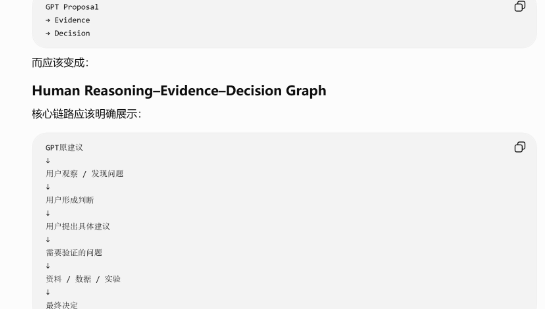
\includegraphics[width=136.500mm]{assets/crops/W13_02_01.png}};
\node[anchor=north west,inner sep=0,text width=136.50mm,align=left] at (14.00,129.30) {\color{Muted}\fontsize{7.2}{9.5}\selectfont  后续：我选择保留的图型};
\node[anchor=north west,inner sep=0] at (14.000,133.501) {
\includegraphics[width=79.867mm]{assets/crops/W13_02_02.png}};
\node[anchor=north west,inner sep=0,text width=36.40mm,align=left] at (159.60,48.51) {\color{Blue}\fontsize{9.5}{13}\selectfont \bfseries 分别选择合适的图型};
\node[anchor=north west,inner sep=0,text width=36.40mm,align=left] at (159.60,57.16) {\color{Ink}\fontsize{8.7}{12.8}\selectfont  一般过程、人的推理与证据、横向候选树分别保留，各自解释不同类型的问题。};
\draw[draw=Blue,line width=.66pt,rounded corners=1mm,-{Stealth[length=1.8mm,width=1.35mm]}] (157.400,52.009) -- (153.200,52.009) -- (153.200,141.923) -- (43.333,141.923);
\draw[Rule,line width=.35pt] (14,283)--(196,283);
\node[anchor=north west,inner sep=0,text width=170.00mm,align=left] at (14.00,287.00) {\color{Muted}\fontsize{6.7}{8.5}\selectfont  智慧城市与位置服务  /  实验一过程报告  /  Part I};
\node[anchor=north west,inner sep=0,text width=11.00mm,align=left] at (185.00,286.50) {\color{Muted}\fontsize{8}{9}\selectfont  16};
\PageEnd

\PageStart
\node[anchor=north west,inner sep=0,text width=182.00mm,align=left] at (14.00,11.00) {\color{Rose}\fontsize{7.8}{10}\selectfont \bfseries PART I · 工作流构建  /  可追溯交付与研究入口};
\node[anchor=north west,inner sep=0,text width=182.00mm,align=left] at (14.00,22.00) {\color{Ink}\fontsize{17.5}{22.5}\selectfont \bfseries 让GPT对照真实仓库检查成果};
\node[anchor=north west,inner sep=0,text width=182.00mm,align=left] at (14.00,33.51) {\color{Ink}\fontsize{9.5}{14.6}\selectfont  我进一步要求 GPT 检查真实远程成果。重要阶段先保存并发布代码、运行记录和报告，再回来对照证据审核；仓库也由此成为持续复现和检查的入口。};
\node[anchor=north west,inner sep=0] at (14,8) {\hypertarget{W14}{}};
\node[anchor=north west,inner sep=0,text width=136.50mm,align=left] at (14.00,48.63) {\color{Muted}\fontsize{7.2}{9.5}\selectfont  我的原始补充：上传后审核};
\node[anchor=north west,inner sep=0] at (55.811,52.828) {
\includegraphics[width=94.689mm]{assets/crops/W14_01_01.png}};
\node[anchor=north west,inner sep=0,text width=136.50mm,align=left] at (14.00,74.01) {\color{Muted}\fontsize{7.2}{9.5}\selectfont  GPT整理真实远程检查链};
\node[anchor=north west,inner sep=0] at (14.000,78.215) {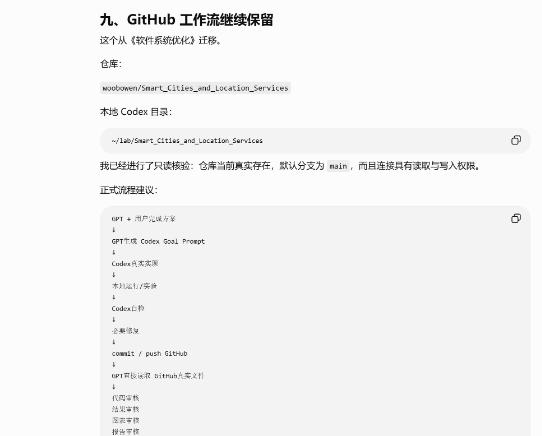
\includegraphics[width=136.500mm]{assets/crops/W14_01_02.png}};
\node[anchor=north west,inner sep=0,text width=36.40mm,align=left] at (159.60,54.63) {\color{Blue}\fontsize{9.5}{13}\selectfont \bfseries 审核要找到实际产物};
\node[anchor=north west,inner sep=0,text width=36.40mm,align=left] at (159.60,63.28) {\color{Ink}\fontsize{8.7}{12.8}\selectfont  我要求代码、输入、输出和图表都能被读取。GPT据此把远程检查接在Codex发布之后。};
\draw[draw=Blue,line width=.66pt,rounded corners=1mm,-{Stealth[length=1.8mm,width=1.35mm]}] (157.400,58.128) -- (153.200,58.128) -- (153.200,54.827) -- (145.889,54.827);
\draw[Rule,line width=.35pt] (14,283)--(196,283);
\node[anchor=north west,inner sep=0,text width=170.00mm,align=left] at (14.00,287.00) {\color{Muted}\fontsize{6.7}{8.5}\selectfont  智慧城市与位置服务  /  实验一过程报告  /  Part I};
\node[anchor=north west,inner sep=0,text width=11.00mm,align=left] at (185.00,286.50) {\color{Muted}\fontsize{8}{9}\selectfont  17};
\PageEnd

\PageStart
\node[anchor=north west,inner sep=0,text width=182.00mm,align=left] at (14.00,11.00) {\color{Rose}\fontsize{7.8}{10}\selectfont \bfseries PART I · 工作流构建  /  可追溯交付与研究入口};
\node[anchor=north west,inner sep=0,text width=182.00mm,align=left] at (14.00,22.00) {\color{Ink}\fontsize{17.5}{22.5}\selectfont \bfseries 让GPT对照真实仓库检查成果（续）};
\node[anchor=north west,inner sep=0,text width=182.00mm,align=left] at (14.00,33.51) {\color{Muted}\fontsize{8.2}{11}\selectfont  接前页，继续阅读这组对话。};
\node[anchor=north west,inner sep=0,text width=136.50mm,align=left] at (14.00,42.51) {\color{Muted}\fontsize{7.2}{9.5}\selectfont  GPT整理真实远程检查链 · 续页};
\node[anchor=north west,inner sep=0] at (14.000,46.709) {
\includegraphics[width=136.500mm]{assets/crops/W14_02_01.png}};
\node[anchor=north west,inner sep=0,text width=136.50mm,align=left] at (14.00,72.31) {\color{Muted}\fontsize{7.2}{9.5}\selectfont  完整工程与教师提交包分工};
\node[anchor=north west,inner sep=0] at (14.000,76.509) {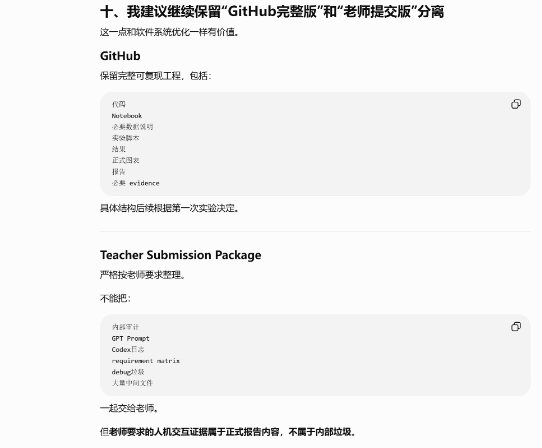
\includegraphics[width=136.500mm]{assets/crops/W14_02_02.png}};
\node[anchor=north west,inner sep=0,text width=36.40mm,align=left] at (159.60,48.51) {\color{Blue}\fontsize{9.5}{13}\selectfont \bfseries 分别组织工程与提交包};
\node[anchor=north west,inner sep=0,text width=36.40mm,align=left] at (159.60,57.16) {\color{Ink}\fontsize{8.7}{12.8}\selectfont  仓库保留复现与审核所需的完整工程；教师提交包则按作业要求整理必要文件。};
\draw[draw=Blue,line width=.66pt,rounded corners=1mm,-{Stealth[length=1.8mm,width=1.35mm]}] (157.400,52.009) -- (153.200,52.009) -- (153.200,164.529) -- (51.273,164.529);
\draw[Rule,line width=.35pt] (14,283)--(196,283);
\node[anchor=north west,inner sep=0,text width=170.00mm,align=left] at (14.00,287.00) {\color{Muted}\fontsize{6.7}{8.5}\selectfont  智慧城市与位置服务  /  实验一过程报告  /  Part I};
\node[anchor=north west,inner sep=0,text width=11.00mm,align=left] at (185.00,286.50) {\color{Muted}\fontsize{8}{9}\selectfont  18};
\PageEnd

\PageStart
\node[anchor=north west,inner sep=0,text width=182.00mm,align=left] at (14.00,11.00) {\color{Rose}\fontsize{7.8}{10}\selectfont \bfseries PART I · 工作流构建  /  可追溯交付与研究入口};
\node[anchor=north west,inner sep=0,text width=182.00mm,align=left] at (14.00,22.00) {\color{Ink}\fontsize{17.5}{22.5}\selectfont \bfseries 把理解检查安排进协作过程};
\node[anchor=north west,inner sep=0,text width=182.00mm,align=left] at (14.00,33.51) {\color{Ink}\fontsize{9.5}{14.6}\selectfont  在旧课程里，我就注意到工程进度与自己的理解可能不同步。迁移后我继续保留这项安排：检查可运行的成果，也请 GPT 帮我讲清原理、方法和结果。};
\node[anchor=north west,inner sep=0] at (14,8) {\hypertarget{W15}{}};
\node[anchor=north west,inner sep=0,text width=136.50mm,align=left] at (14.00,48.63) {\color{Muted}\fontsize{7.2}{9.5}\selectfont  我提出进度不同步，GPT调整};
\node[anchor=north west,inner sep=0] at (14.000,52.828) {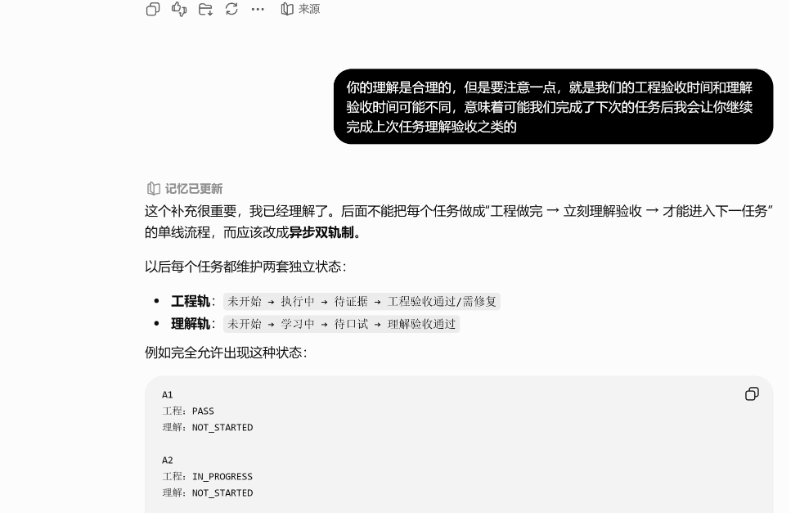
\includegraphics[width=136.500mm]{assets/crops/W15_01_01.png}};
\node[anchor=north west,inner sep=0,text width=136.50mm,align=left] at (14.00,146.78) {\color{Muted}\fontsize{7.2}{9.5}\selectfont  新项目继续保留独立状态};
\node[anchor=north west,inner sep=0] at (14.000,150.979) {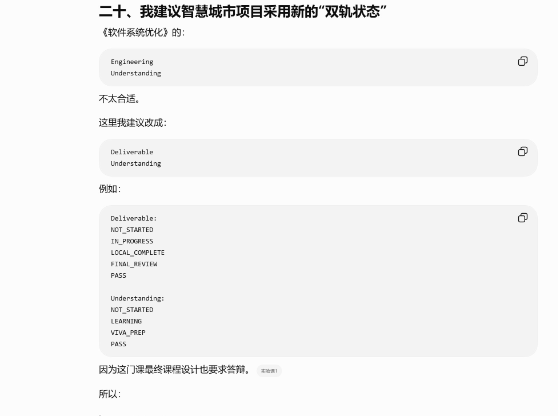
\includegraphics[width=136.500mm]{assets/crops/W15_01_02.png}};
\node[anchor=north west,inner sep=0,text width=36.40mm,align=left] at (159.60,54.63) {\color{Blue}\fontsize{9.5}{13}\selectfont \bfseries 用解释检查我的理解};
\node[anchor=north west,inner sep=0,text width=36.40mm,align=left] at (159.60,63.28) {\color{Ink}\fontsize{8.7}{12.8}\selectfont  我需要能自己讲清方法和结果。GPT因此保留讲解与答辩准备这一职责，和工程核查一起推进。};
\draw[draw=Blue,line width=.66pt,rounded corners=1mm,-{Stealth[length=1.8mm,width=1.35mm]}] (157.400,58.128) -- (153.200,58.128) -- (153.200,67.880) -- (144.791,67.880);
\node[anchor=north west,inner sep=0,text width=36.40mm,align=left] at (159.60,100.37) {\color{Violet}\fontsize{9.5}{13}\selectfont \bfseries 分别跟进各项进度};
\node[anchor=north west,inner sep=0,text width=36.40mm,align=left] at (159.60,109.02) {\color{Ink}\fontsize{8.7}{12.8}\selectfont  后来我们把成果、理解和提交分别记录。我可以先检查工程结果，再安排方法复盘和文档审阅。};
\draw[draw=Violet,line width=.66pt,rounded corners=1mm,-{Stealth[length=1.8mm,width=1.35mm]}] (157.400,103.872) -- (155.300,103.872) -- (155.300,190.853) -- (54.363,190.853);
\draw[Rule,line width=.35pt] (14,283)--(196,283);
\node[anchor=north west,inner sep=0,text width=170.00mm,align=left] at (14.00,287.00) {\color{Muted}\fontsize{6.7}{8.5}\selectfont  智慧城市与位置服务  /  实验一过程报告  /  Part I};
\node[anchor=north west,inner sep=0,text width=11.00mm,align=left] at (185.00,286.50) {\color{Muted}\fontsize{8}{9}\selectfont  19};
\PageEnd

\PageStart
\node[anchor=north west,inner sep=0,text width=182.00mm,align=left] at (14.00,11.00) {\color{Rose}\fontsize{7.8}{10}\selectfont \bfseries PART I · 工作流构建  /  可追溯交付与研究入口};
\node[anchor=north west,inner sep=0,text width=182.00mm,align=left] at (14.00,22.00) {\color{Ink}\fontsize{17.5}{22.5}\selectfont \bfseries 带着已有规则进入真实实验};
\node[anchor=north west,inner sep=0,text width=182.00mm,align=left] at (14.00,33.51) {\color{Ink}\fontsize{9.5}{14.6}\selectfont  进入实验一之前，我已对证据、图形和文档形成基本要求。接下来，我希望在真实任务中检查这套做法怎样处理研究判断、执行反馈和失败，再据此继续修改工作流。};
\node[anchor=north west,inner sep=0] at (14,8) {\hypertarget{W16}{}};
\node[anchor=north west,inner sep=0,text width=136.50mm,align=left] at (14.00,48.63) {\color{Muted}\fontsize{7.2}{9.5}\selectfont  我要求看到真实页面效果};
\node[anchor=north west,inner sep=0] at (14.000,52.828) {
\includegraphics[width=82.771mm]{assets/crops/W16_01_01.png}};
\node[anchor=north west,inner sep=0,text width=136.50mm,align=left] at (14.00,93.17) {\color{Muted}\fontsize{7.2}{9.5}\selectfont  局部决策与总体故事的分工};
\node[anchor=north west,inner sep=0] at (14.000,97.370) {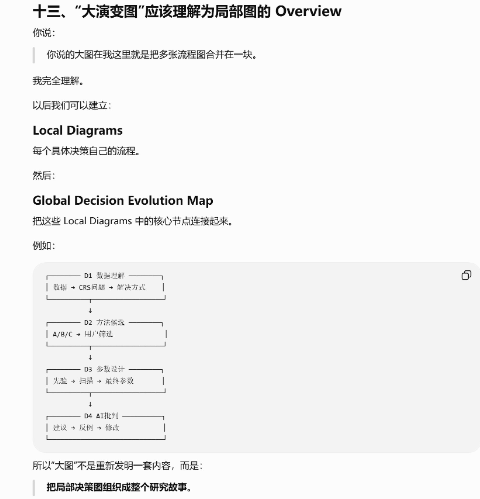
\includegraphics[width=136.500mm]{assets/crops/W16_01_02.png}};
\node[anchor=north west,inner sep=0,text width=36.40mm,align=left] at (159.60,54.63) {\color{Blue}\fontsize{9.5}{13}\selectfont \bfseries 先看实际产物};
\node[anchor=north west,inner sep=0,text width=36.40mm,align=left] at (159.60,63.28) {\color{Ink}\fontsize{8.7}{12.8}\selectfont  我要求看到真实页面，再检查内容和对应关系。GPT据此安排局部证据与总体说明的制作顺序。};
\draw[draw=Blue,line width=.66pt,rounded corners=1mm,-{Stealth[length=1.8mm,width=1.35mm]}] (157.400,58.128) -- (153.200,58.128) -- (153.200,59.072) -- (95.319,59.072);
\node[anchor=north west,inner sep=0,text width=36.40mm,align=left] at (159.60,100.37) {\color{Violet}\fontsize{9.5}{13}\selectfont \bfseries 由具体决定归纳整体};
\node[anchor=north west,inner sep=0,text width=36.40mm,align=left] at (159.60,109.02) {\color{Ink}\fontsize{8.7}{12.8}\selectfont  先看清每个问题怎样形成决定，再归纳总体演化。实验一随后为这套工作方式带来了新的检验。};
\draw[draw=Violet,line width=.66pt,rounded corners=1mm,-{Stealth[length=1.8mm,width=1.35mm]}] (157.400,103.872) -- (155.300,103.872) -- (155.300,235.718) -- (69.169,235.718);
\draw[Rule,line width=.35pt] (14,283)--(196,283);
\node[anchor=north west,inner sep=0,text width=170.00mm,align=left] at (14.00,287.00) {\color{Muted}\fontsize{6.7}{8.5}\selectfont  智慧城市与位置服务  /  实验一过程报告  /  Part I};
\node[anchor=north west,inner sep=0,text width=11.00mm,align=left] at (185.00,286.50) {\color{Muted}\fontsize{8}{9}\selectfont  20};
\PageEnd

\PageStart
\node[anchor=north west,inner sep=0,text width=182.00mm,align=left] at (14.00,11.00) {\color{Blue}\fontsize{7.8}{10}\selectfont \bfseries PART II · 实验一中的交互与决策  /  任务理解与研究起点};
\node[anchor=north west,inner sep=0,text width=182.00mm,align=left] at (14.00,22.00) {\color{Ink}\fontsize{17.5}{22.5}\selectfont \bfseries 从完整读题开始推进实验一};
\node[anchor=north west,inner sep=0,text width=182.00mm,align=left] at (14.00,33.51) {\color{Ink}\fontsize{9.5}{14.6}\selectfont  带着前面形成的分工和研究规则，我开始与 GPT 推进实验一。我先交给它老师材料、原始数据和已有工程，要求读清任务，再分别核对 Notebook、Agent、模板和历史输出的实际用途。};
\node[anchor=north west,inner sep=0] at (14,8) {\hypertarget{E01}{}};
\node[anchor=north west,inner sep=0,text width=136.50mm,align=left] at (14.00,48.63) {\color{Muted}\fontsize{7.2}{9.5}\selectfont  我发出的研究初始化提示词节选};
\node[anchor=north west,inner sep=0] at (14.000,52.828) {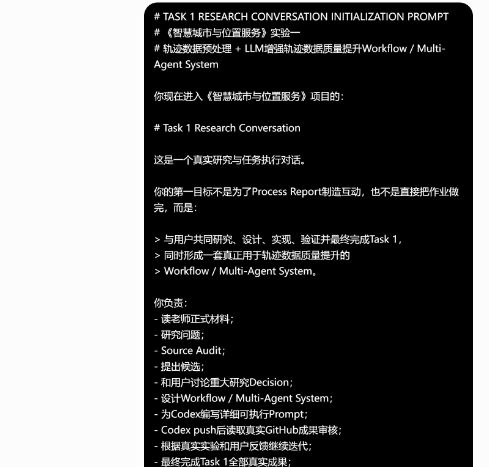
\includegraphics[width=136.500mm]{assets/crops/E01_01_01.png}};
\node[anchor=north west,inner sep=0,text width=36.40mm,align=left] at (159.60,54.63) {\color{Blue}\fontsize{9.5}{13}\selectfont \bfseries 先把任务理解完整};
\node[anchor=north west,inner sep=0,text width=36.40mm,align=left] at (159.60,63.28) {\color{Ink}\fontsize{8.7}{12.8}\selectfont  我要求共同研究、设计、实现和验证。GPT先完成材料阅读与任务梳理，为后面的方案讨论准备依据。};
\draw[draw=Blue,line width=.66pt,rounded corners=1mm,-{Stealth[length=1.8mm,width=1.35mm]}] (157.400,58.128) -- (153.200,58.128) -- (153.200,110.610) -- (69.828,110.610);
\draw[Rule,line width=.35pt] (14,283)--(196,283);
\node[anchor=north west,inner sep=0,text width=170.00mm,align=left] at (14.00,287.00) {\color{Muted}\fontsize{6.7}{8.5}\selectfont  智慧城市与位置服务  /  实验一过程报告  /  Part II};
\node[anchor=north west,inner sep=0,text width=11.00mm,align=left] at (185.00,286.50) {\color{Muted}\fontsize{8}{9}\selectfont  21};
\PageEnd

\PageStart
\node[anchor=north west,inner sep=0,text width=182.00mm,align=left] at (14.00,11.00) {\color{Blue}\fontsize{7.8}{10}\selectfont \bfseries PART II · 实验一中的交互与决策  /  任务理解与研究起点};
\node[anchor=north west,inner sep=0,text width=182.00mm,align=left] at (14.00,22.00) {\color{Ink}\fontsize{17.5}{22.5}\selectfont \bfseries 从完整读题开始推进实验一（续）};
\node[anchor=north west,inner sep=0,text width=182.00mm,align=left] at (14.00,33.51) {\color{Muted}\fontsize{8.2}{11}\selectfont  接前页，继续阅读这组对话。};
\node[anchor=north west,inner sep=0,text width=136.50mm,align=left] at (14.00,42.51) {\color{Muted}\fontsize{7.2}{9.5}\selectfont  我发出的研究初始化提示词节选 · 续页};
\node[anchor=north west,inner sep=0] at (14.000,46.709) {
\includegraphics[width=136.500mm]{assets/crops/E01_02_01.png}};
\node[anchor=north west,inner sep=0,text width=136.50mm,align=left] at (14.00,69.77) {\color{Muted}\fontsize{7.2}{9.5}\selectfont  GPT的Stage 0/1阅读反馈};
\node[anchor=north west,inner sep=0] at (14.000,73.974) {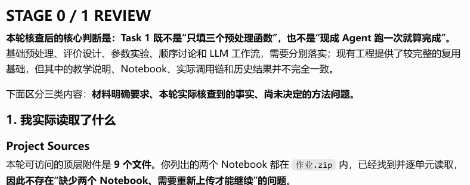
\includegraphics[width=136.500mm]{assets/crops/E01_02_02.png}};
\node[anchor=north west,inner sep=0,text width=136.50mm,align=left] at (14.00,132.90) {\color{Muted}\fontsize{7.2}{9.5}\selectfont  同一轮：确认事实而非冻结方法};
\node[anchor=north west,inner sep=0] at (14.000,137.103) {
\includegraphics[width=136.500mm]{assets/crops/E01_02_03.png}};
\node[anchor=north west,inner sep=0,text width=36.40mm,align=left] at (159.60,48.51) {\color{Blue}\fontsize{9.5}{13}\selectfont \bfseries 按用途核对现有材料};
\node[anchor=north west,inner sep=0,text width=36.40mm,align=left] at (159.60,57.16) {\color{Ink}\fontsize{8.7}{12.8}\selectfont  真实输入、可复用代码和历史演示分别整理；分段、去噪、简化之外，评价、参数、顺序和LLM工作流也进入任务清单。};
\draw[draw=Blue,line width=.66pt,rounded corners=1mm,-{Stealth[length=1.8mm,width=1.35mm]}] (157.400,52.009) -- (153.200,52.009) -- (153.200,167.453) -- (82.831,167.453);
\draw[Rule,line width=.35pt] (14,283)--(196,283);
\node[anchor=north west,inner sep=0,text width=170.00mm,align=left] at (14.00,287.00) {\color{Muted}\fontsize{6.7}{8.5}\selectfont  智慧城市与位置服务  /  实验一过程报告  /  Part II};
\node[anchor=north west,inner sep=0,text width=11.00mm,align=left] at (185.00,286.50) {\color{Muted}\fontsize{8}{9}\selectfont  22};
\PageEnd

\PageStart
\node[anchor=north west,inner sep=0,text width=182.00mm,align=left] at (14.00,11.00) {\color{Blue}\fontsize{7.8}{10}\selectfont \bfseries PART II · 实验一中的交互与决策  /  任务理解与研究起点};
\node[anchor=north west,inner sep=0,text width=182.00mm,align=left] at (14.00,22.00) {\color{Ink}\fontsize{17.5}{22.5}\selectfont \bfseries GPT先解释依据，我再判断方案};
\node[anchor=north west,inner sep=0,text width=182.00mm,align=left] at (14.00,33.51) {\color{Ink}\fontsize{9.5}{14.6}\selectfont  GPT列出了坐标、参数、顺序和评价等问题，但这些专业问题需要先讲清楚。我因此要求它解释依据、给出推荐和风险，再由我判断，同时继续沿用 GPT 与 Codex 的分工。};
\node[anchor=north west,inner sep=0] at (14,8) {\hypertarget{E02}{}};
\node[anchor=north west,inner sep=0,text width=136.50mm,align=left] at (14.00,48.63) {\color{Muted}\fontsize{7.2}{9.5}\selectfont  我的补充与GPT的直接回应};
\node[anchor=north west,inner sep=0] at (14.000,52.828) {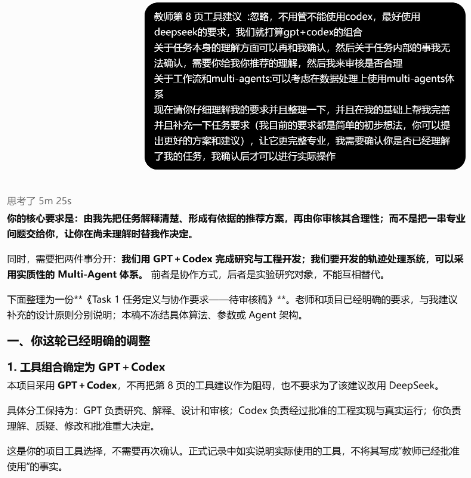
\includegraphics[width=136.500mm]{assets/crops/E02_01_01.png}};
\node[anchor=north west,inner sep=0,text width=136.50mm,align=left] at (14.00,196.56) {\color{Muted}\fontsize{7.2}{9.5}\selectfont  同一回答：先研究、解释和推荐};
\node[anchor=north west,inner sep=0] at (14.000,200.757) {
\includegraphics[width=136.500mm]{assets/crops/E02_01_02.png}};
\node[anchor=north west,inner sep=0,text width=36.40mm,align=left] at (159.60,54.63) {\color{Blue}\fontsize{9.5}{13}\selectfont \bfseries 我需要推荐及其理由};
\node[anchor=north west,inner sep=0,text width=36.40mm,align=left] at (159.60,63.28) {\color{Ink}\fontsize{8.7}{12.8}\selectfont  面对专业问题，我希望先知道为什么要讨论、已有证据是什么，以及不同选择会怎样影响实验。};
\draw[draw=Blue,line width=.66pt,rounded corners=1mm,-{Stealth[length=1.8mm,width=1.35mm]}] (157.400,58.128) -- (153.200,58.128) -- (153.200,70.941) -- (131.662,70.941);
\node[anchor=north west,inner sep=0,text width=36.40mm,align=left] at (159.60,100.37) {\color{Violet}\fontsize{9.5}{13}\selectfont \bfseries 解释帮助我作判断};
\node[anchor=north west,inner sep=0,text width=36.40mm,align=left] at (159.60,109.02) {\color{Ink}\fontsize{8.7}{12.8}\selectfont  GPT把问题、影响、证据、推荐与风险一起说明。重要选择集中讨论，已经确定的普通动作继续执行。};
\draw[draw=Violet,line width=.66pt,rounded corners=1mm,-{Stealth[length=1.8mm,width=1.35mm]}] (157.400,103.872) -- (155.300,103.872) -- (155.300,256.255) -- (131.662,256.255);
\draw[Rule,line width=.35pt] (14,283)--(196,283);
\node[anchor=north west,inner sep=0,text width=170.00mm,align=left] at (14.00,287.00) {\color{Muted}\fontsize{6.7}{8.5}\selectfont  智慧城市与位置服务  /  实验一过程报告  /  Part II};
\node[anchor=north west,inner sep=0,text width=11.00mm,align=left] at (185.00,286.50) {\color{Muted}\fontsize{8}{9}\selectfont  23};
\PageEnd

\PageStart
\node[anchor=north west,inner sep=0,text width=182.00mm,align=left] at (14.00,11.00) {\color{Blue}\fontsize{7.8}{10}\selectfont \bfseries PART II · 实验一中的交互与决策  /  面向实验任务的Multi-Agent构建};
\node[anchor=north west,inner sep=0,text width=182.00mm,align=left] at (14.00,22.00) {\color{Ink}\fontsize{17.5}{22.5}\selectfont \bfseries 让Multi-Agent从一开始参与实验任务};
\node[anchor=north west,inner sep=0,text width=182.00mm,align=left] at (14.00,33.51) {\color{Ink}\fontsize{9.5}{14.6}\selectfont  最初 GPT 把任务理解成先完成分段、去噪和简化，再建立 Agent。我马上纠正：Multi-Agent应当帮助我完成实验，从研究、数据处理到实验和检查都要参与，而不是最后补一层解释。};
\node[anchor=north west,inner sep=0] at (14,8) {\hypertarget{E03}{}};
\node[anchor=north west,inner sep=0,text width=136.50mm,align=left] at (14.00,48.63) {\color{Muted}\fontsize{7.2}{9.5}\selectfont  我纠正任务定位，GPT重新定义目标};
\node[anchor=north west,inner sep=0] at (14.000,52.828) {
\includegraphics[width=136.500mm]{assets/crops/E03_01_01.png}};
\node[anchor=north west,inner sep=0,text width=36.40mm,align=left] at (159.60,54.63) {\color{Blue}\fontsize{9.5}{13}\selectfont \bfseries 我修改了任务组织方式};
\node[anchor=north west,inner sep=0,text width=36.40mm,align=left] at (159.60,63.28) {\color{Ink}\fontsize{8.7}{12.8}\selectfont  我把体系的职责扩展到任务拆解、资料研究、真实处理和结果检验，要求这些工作就在协作过程中完成。};
\draw[draw=Blue,line width=.66pt,rounded corners=1mm,-{Stealth[length=1.8mm,width=1.35mm]}] (157.400,58.128) -- (153.200,58.128) -- (153.200,134.120) -- (53.704,134.120);
\draw[Rule,line width=.35pt] (14,283)--(196,283);
\node[anchor=north west,inner sep=0,text width=170.00mm,align=left] at (14.00,287.00) {\color{Muted}\fontsize{6.7}{8.5}\selectfont  智慧城市与位置服务  /  实验一过程报告  /  Part II};
\node[anchor=north west,inner sep=0,text width=11.00mm,align=left] at (185.00,286.50) {\color{Muted}\fontsize{8}{9}\selectfont  24};
\PageEnd

\PageStart
\node[anchor=north west,inner sep=0,text width=182.00mm,align=left] at (14.00,11.00) {\color{Blue}\fontsize{7.8}{10}\selectfont \bfseries PART II · 实验一中的交互与决策  /  面向实验任务的Multi-Agent构建};
\node[anchor=north west,inner sep=0,text width=182.00mm,align=left] at (14.00,22.00) {\color{Ink}\fontsize{17.5}{22.5}\selectfont \bfseries 让Multi-Agent从一开始参与实验任务（续）};
\node[anchor=north west,inner sep=0,text width=182.00mm,align=left] at (14.00,33.51) {\color{Muted}\fontsize{8.2}{11}\selectfont  接前页，继续阅读这组对话。};
\node[anchor=north west,inner sep=0,text width=136.50mm,align=left] at (14.00,42.51) {\color{Muted}\fontsize{7.2}{9.5}\selectfont  我纠正任务定位，GPT重新定义目标 · 续页};
\node[anchor=north west,inner sep=0] at (14.000,46.709) {
\includegraphics[width=136.500mm]{assets/crops/E03_02_01.png}};
\node[anchor=north west,inner sep=0,text width=136.50mm,align=left] at (14.00,97.70) {\color{Muted}\fontsize{7.2}{9.5}\selectfont  同一回答：必须真正采取行动};
\node[anchor=north west,inner sep=0] at (14.000,101.899) {
\includegraphics[width=136.500mm]{assets/crops/E03_02_02.png}};
\node[anchor=north west,inner sep=0,text width=36.40mm,align=left] at (159.60,48.51) {\color{Blue}\fontsize{9.5}{13}\selectfont \bfseries 开发与运行的分工};
\node[anchor=north west,inner sep=0,text width=36.40mm,align=left] at (159.60,57.16) {\color{Ink}\fontsize{8.7}{12.8}\selectfont  GPT与Codex负责研究和工程开发；实验中的Agent则需要发起任务、读取真实结果，并据此决定下一步。};
\draw[draw=Blue,line width=.66pt,rounded corners=1mm,-{Stealth[length=1.8mm,width=1.35mm]}] (157.400,52.009) -- (153.200,52.009) -- (153.200,169.280) -- (149.631,169.280);
\node[anchor=north west,inner sep=0,text width=36.40mm,align=left] at (159.60,94.25) {\color{Rose}\fontsize{8.9}{12.5}\selectfont \bfseries 我的回看};
\node[anchor=north west,inner sep=0,text width=36.40mm,align=left] at (159.60,101.25) {\color{Ink}\fontsize{8.5}{12.7}\selectfont  这轮讨论把设计重点转向了职责、行动与核验，也为后续原型明确了需要检查的内容。};
\draw[Rule,line width=.35pt] (14,283)--(196,283);
\node[anchor=north west,inner sep=0,text width=170.00mm,align=left] at (14.00,287.00) {\color{Muted}\fontsize{6.7}{8.5}\selectfont  智慧城市与位置服务  /  实验一过程报告  /  Part II};
\node[anchor=north west,inner sep=0,text width=11.00mm,align=left] at (185.00,286.50) {\color{Muted}\fontsize{8}{9}\selectfont  25};
\PageEnd

\PageStart
\node[anchor=north west,inner sep=0,text width=182.00mm,align=left] at (14.00,11.00) {\color{Blue}\fontsize{7.8}{10}\selectfont \bfseries PART II · 实验一中的交互与决策  /  面向实验任务的Multi-Agent构建};
\node[anchor=north west,inner sep=0,text width=182.00mm,align=left] at (14.00,22.00) {\color{Ink}\fontsize{17.5}{22.5}\selectfont \bfseries 把结果反馈接回下一轮研究};
\node[anchor=north west,inner sep=0,text width=182.00mm,align=left] at (14.00,33.51) {\color{Ink}\fontsize{9.5}{14.6}\selectfont  我又补充：体系在第一次形成结果后，还要能够继续检查和改进。理解任务、实际完成、审查结果、找出下一步问题，再继续验证，都应属于同一个工作流。};
\node[anchor=north west,inner sep=0] at (14,8) {\hypertarget{E04}{}};
\node[anchor=north west,inner sep=0,text width=136.50mm,align=left] at (14.00,48.63) {\color{Muted}\fontsize{7.2}{9.5}\selectfont  我的持续改进要求与GPT修订};
\node[anchor=north west,inner sep=0] at (14.000,52.828) {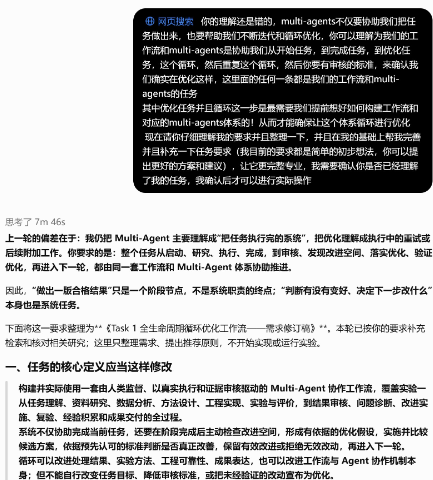
\includegraphics[width=136.500mm]{assets/crops/E04_01_01.png}};
\node[anchor=north west,inner sep=0,text width=36.40mm,align=left] at (159.60,54.63) {\color{Blue}\fontsize{9.5}{13}\selectfont \bfseries 让改进贯穿任务};
\node[anchor=north west,inner sep=0,text width=36.40mm,align=left] at (159.60,63.28) {\color{Ink}\fontsize{8.7}{12.8}\selectfont  我希望从开始到完成再到改进都在同一体系里。GPT因此把结果检查和下一步选择接回主循环。};
\draw[draw=Blue,line width=.66pt,rounded corners=1mm,-{Stealth[length=1.8mm,width=1.35mm]}] (157.400,58.128) -- (153.200,58.128) -- (153.200,91.288) -- (144.510,91.288);
\draw[Rule,line width=.35pt] (14,283)--(196,283);
\node[anchor=north west,inner sep=0,text width=170.00mm,align=left] at (14.00,287.00) {\color{Muted}\fontsize{6.7}{8.5}\selectfont  智慧城市与位置服务  /  实验一过程报告  /  Part II};
\node[anchor=north west,inner sep=0,text width=11.00mm,align=left] at (185.00,286.50) {\color{Muted}\fontsize{8}{9}\selectfont  26};
\PageEnd

\PageStart
\node[anchor=north west,inner sep=0,text width=182.00mm,align=left] at (14.00,11.00) {\color{Blue}\fontsize{7.8}{10}\selectfont \bfseries PART II · 实验一中的交互与决策  /  面向实验任务的Multi-Agent构建};
\node[anchor=north west,inner sep=0,text width=182.00mm,align=left] at (14.00,22.00) {\color{Ink}\fontsize{17.5}{22.5}\selectfont \bfseries 把结果反馈接回下一轮研究（续）};
\node[anchor=north west,inner sep=0,text width=182.00mm,align=left] at (14.00,33.51) {\color{Muted}\fontsize{8.2}{11}\selectfont  接前页，继续阅读这组对话。};
\node[anchor=north west,inner sep=0,text width=136.50mm,align=left] at (14.00,42.51) {\color{Muted}\fontsize{7.2}{9.5}\selectfont  我的持续改进要求与GPT修订 · 续页};
\node[anchor=north west,inner sep=0] at (14.000,46.709) {
\includegraphics[width=136.500mm]{assets/crops/E04_02_01.png}};
\node[anchor=north west,inner sep=0,text width=136.50mm,align=left] at (14.00,83.43) {\color{Muted}\fontsize{7.2}{9.5}\selectfont  同一回答：把反馈接回下一轮};
\node[anchor=north west,inner sep=0] at (14.000,87.634) {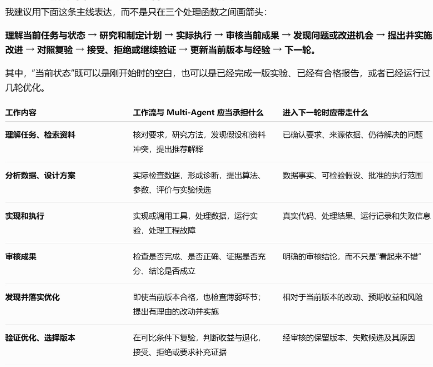
\includegraphics[width=136.500mm]{assets/crops/E04_02_02.png}};
\node[anchor=north west,inner sep=0,text width=36.40mm,align=left] at (159.60,48.51) {\color{Blue}\fontsize{9.5}{13}\selectfont \bfseries 由具体问题引出下一轮};
\node[anchor=north west,inner sep=0,text width=36.40mm,align=left] at (159.60,57.16) {\color{Ink}\fontsize{8.7}{12.8}\selectfont  当前结果、失败原因和待验证假设成为下一轮输入。体系需要说明准备改什么，以及怎样检验。};
\draw[draw=Blue,line width=.66pt,rounded corners=1mm,-{Stealth[length=1.8mm,width=1.35mm]}] (157.400,52.009) -- (153.200,52.009) -- (153.200,98.667) -- (149.554,98.667);
\draw[Rule,line width=.35pt] (14,283)--(196,283);
\node[anchor=north west,inner sep=0,text width=170.00mm,align=left] at (14.00,287.00) {\color{Muted}\fontsize{6.7}{8.5}\selectfont  智慧城市与位置服务  /  实验一过程报告  /  Part II};
\node[anchor=north west,inner sep=0,text width=11.00mm,align=left] at (185.00,286.50) {\color{Muted}\fontsize{8}{9}\selectfont  27};
\PageEnd

\PageStart
\node[anchor=north west,inner sep=0,text width=182.00mm,align=left] at (14.00,11.00) {\color{Blue}\fontsize{7.8}{10}\selectfont \bfseries PART II · 实验一中的交互与决策  /  面向实验任务的Multi-Agent构建};
\node[anchor=north west,inner sep=0,text width=182.00mm,align=left] at (14.00,22.00) {\color{Ink}\fontsize{17.5}{22.5}\selectfont \bfseries 从轨迹任务反推研究问题};
\node[anchor=north west,inner sep=0,text width=182.00mm,align=left] at (14.00,33.51) {\color{Ink}\fontsize{9.5}{14.6}\selectfont  当讨论越来越像在搭通用 Multi-Agent 平台时，我把方向拉回实验一：先列出实际需要完成的工作，再围绕这些任务确定该检索和验证什么。};
\node[anchor=north west,inner sep=0] at (14,8) {\hypertarget{E05}{}};
\node[anchor=north west,inner sep=0,text width=136.50mm,align=left] at (14.00,48.63) {\color{Muted}\fontsize{7.2}{9.5}\selectfont  我要求先明确实验的实际任务};
\node[anchor=north west,inner sep=0] at (14.000,52.828) {
\includegraphics[width=136.500mm]{assets/crops/E05_01_01.png}};
\node[anchor=north west,inner sep=0,text width=36.40mm,align=left] at (159.60,54.63) {\color{Blue}\fontsize{9.5}{13}\selectfont \bfseries 先问实验需要什么};
\node[anchor=north west,inner sep=0,text width=36.40mm,align=left] at (159.60,63.28) {\color{Ink}\fontsize{8.7}{12.8}\selectfont  我关心怎样处理和优化轨迹数据，因此要求GPT先说明实际任务及其困难，再寻找相关方法。};
\draw[draw=Blue,line width=.66pt,rounded corners=1mm,-{Stealth[length=1.8mm,width=1.35mm]}] (157.400,58.128) -- (153.200,58.128) -- (153.200,70.620) -- (149.666,70.620);
\draw[Rule,line width=.35pt] (14,283)--(196,283);
\node[anchor=north west,inner sep=0,text width=170.00mm,align=left] at (14.00,287.00) {\color{Muted}\fontsize{6.7}{8.5}\selectfont  智慧城市与位置服务  /  实验一过程报告  /  Part II};
\node[anchor=north west,inner sep=0,text width=11.00mm,align=left] at (185.00,286.50) {\color{Muted}\fontsize{8}{9}\selectfont  28};
\PageEnd

\PageStart
\node[anchor=north west,inner sep=0,text width=182.00mm,align=left] at (14.00,11.00) {\color{Blue}\fontsize{7.8}{10}\selectfont \bfseries PART II · 实验一中的交互与决策  /  面向实验任务的Multi-Agent构建};
\node[anchor=north west,inner sep=0,text width=182.00mm,align=left] at (14.00,22.00) {\color{Ink}\fontsize{17.5}{22.5}\selectfont \bfseries 从轨迹任务反推研究问题（续）};
\node[anchor=north west,inner sep=0,text width=182.00mm,align=left] at (14.00,33.51) {\color{Muted}\fontsize{8.2}{11}\selectfont  接前页，继续阅读这组对话。};
\node[anchor=north west,inner sep=0,text width=136.50mm,align=left] at (14.00,42.51) {\color{Muted}\fontsize{7.2}{9.5}\selectfont  我要求先明确实验的实际任务 · 续页};
\node[anchor=north west,inner sep=0] at (14.000,46.709) {
\includegraphics[width=136.500mm]{assets/crops/E05_02_01.png}};
\node[anchor=north west,inner sep=0,text width=136.50mm,align=left] at (14.00,84.71) {\color{Muted}\fontsize{7.2}{9.5}\selectfont  GPT把检索拆成任务导向的模块};
\node[anchor=north west,inner sep=0] at (14.000,88.914) {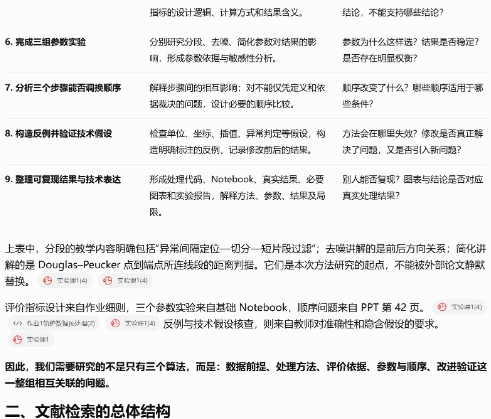
\includegraphics[width=136.500mm]{assets/crops/E05_02_02.png}};
\node[anchor=north west,inner sep=0,text width=36.40mm,align=left] at (159.60,48.51) {\color{Blue}\fontsize{9.5}{13}\selectfont \bfseries 把检索按问题组织};
\node[anchor=north west,inner sep=0,text width=36.40mm,align=left] at (159.60,57.16) {\color{Ink}\fontsize{8.7}{12.8}\selectfont  分段、去噪、简化之外，数据前提、评价、顺序和结果解释也各有问题。GPT据此组织了任务导向的检索模块。};
\draw[draw=Blue,line width=.66pt,rounded corners=1mm,-{Stealth[length=1.8mm,width=1.35mm]}] (157.400,52.009) -- (153.200,52.009) -- (153.200,92.250) -- (138.268,92.250);
\draw[Rule,line width=.35pt] (14,283)--(196,283);
\node[anchor=north west,inner sep=0,text width=170.00mm,align=left] at (14.00,287.00) {\color{Muted}\fontsize{6.7}{8.5}\selectfont  智慧城市与位置服务  /  实验一过程报告  /  Part II};
\node[anchor=north west,inner sep=0,text width=11.00mm,align=left] at (185.00,286.50) {\color{Muted}\fontsize{8}{9}\selectfont  29};
\PageEnd

\PageStart
\node[anchor=north west,inner sep=0,text width=182.00mm,align=left] at (14.00,11.00) {\color{Blue}\fontsize{7.8}{10}\selectfont \bfseries PART II · 实验一中的交互与决策  /  面向实验任务的Multi-Agent构建};
\node[anchor=north west,inner sep=0,text width=182.00mm,align=left] at (14.00,22.00) {\color{Ink}\fontsize{17.5}{22.5}\selectfont \bfseries 从广泛检索收敛到少量可用思路};
\node[anchor=north west,inner sep=0,text width=182.00mm,align=left] at (14.00,33.51) {\color{Ink}\fontsize{9.5}{14.6}\selectfont  看过新旧轨迹研究后，我补充了一条取舍原则：论文应帮助我们解决具体任务，真正进入实验的是少量可解释、可检验的改动。我在执行前收窄使用范围，并据此回看此前汇总的研究材料。};
\node[anchor=north west,inner sep=0] at (14,8) {\hypertarget{E06}{}};
\node[anchor=north west,inner sep=0,text width=136.50mm,align=left] at (14.00,48.63) {\color{Muted}\fontsize{7.2}{9.5}\selectfont  执行前的补充：收窄论文使用范围};
\node[anchor=north west,inner sep=0] at (57.702,52.828) {
\includegraphics[width=92.798mm]{assets/crops/E06_01_01.png}};
\node[anchor=north west,inner sep=0,text width=136.50mm,align=left] at (14.00,76.10) {\color{Muted}\fontsize{7.2}{9.5}\selectfont  回看此前的文献汇总：可迁移思路与适用条件};
\node[anchor=north west,inner sep=0] at (14.000,80.302) {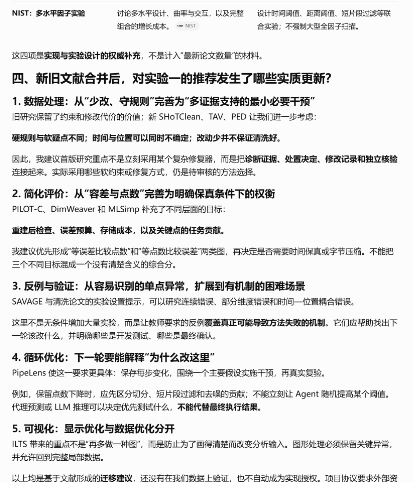
\includegraphics[width=136.500mm]{assets/crops/E06_01_02.png}};
\node[anchor=north west,inner sep=0,text width=36.40mm,align=left] at (159.60,54.63) {\color{Blue}\fontsize{9.5}{13}\selectfont \bfseries 以适用性筛选来源};
\node[anchor=north west,inner sep=0,text width=36.40mm,align=left] at (159.60,63.28) {\color{Ink}\fontsize{8.7}{12.8}\selectfont  我在执行前强调少量有用的思路。论文是否值得采用，要看它与当前问题的关系、实现成本和可验证性。};
\draw[draw=Blue,line width=.66pt,rounded corners=1mm,-{Stealth[length=1.8mm,width=1.35mm]}] (157.400,58.128) -- (153.200,58.128) -- (153.200,67.935) -- (128.919,67.935);
\node[anchor=north west,inner sep=0,text width=36.40mm,align=left] at (159.60,100.37) {\color{Violet}\fontsize{9.5}{13}\selectfont \bfseries 把每项来源的用途说清};
\node[anchor=north west,inner sep=0,text width=36.40mm,align=left] at (159.60,109.02) {\color{Ink}\fontsize{8.7}{12.8}\selectfont  后续分别记录实际采用、借鉴思想、风险提示和未采用，让查阅材料与实验中的具体做法对应起来。};
\draw[draw=Violet,line width=.66pt,rounded corners=1mm,-{Stealth[length=1.8mm,width=1.35mm]}] (157.400,103.872) -- (155.300,103.872) -- (155.300,113.438) -- (118.848,113.438);
\draw[Rule,line width=.35pt] (14,283)--(196,283);
\node[anchor=north west,inner sep=0,text width=170.00mm,align=left] at (14.00,287.00) {\color{Muted}\fontsize{6.7}{8.5}\selectfont  智慧城市与位置服务  /  实验一过程报告  /  Part II};
\node[anchor=north west,inner sep=0,text width=11.00mm,align=left] at (185.00,286.50) {\color{Muted}\fontsize{8}{9}\selectfont  30};
\PageEnd

\PageStart
\node[anchor=north west,inner sep=0,text width=182.00mm,align=left] at (14.00,11.00) {\color{Blue}\fontsize{7.8}{10}\selectfont \bfseries PART II · 实验一中的交互与决策  /  执行与审核机制的落地和修正};
\node[anchor=north west,inner sep=0,text width=182.00mm,align=left] at (14.00,22.00) {\color{Ink}\fontsize{17.5}{22.5}\selectfont \bfseries 用三个Goal组织连续推进};
\node[anchor=north west,inner sep=0,text width=182.00mm,align=left] at (14.00,33.51) {\color{Ink}\fontsize{9.5}{14.6}\selectfont  我确认三段安排：先建立可信基础和最小执行循环，再逐项验证候选，最后检查组合并收敛交付。我同时要求共同评价、针对性审核和先单项后组合，用实际证据决定取舍。};
\node[anchor=north west,inner sep=0] at (14,8) {\hypertarget{E07}{}};
\node[anchor=north west,inner sep=0,text width=136.50mm,align=left] at (14.00,48.63) {\color{Muted}\fontsize{7.2}{9.5}\selectfont  我对阶段安排的完整确认与补充};
\node[anchor=north west,inner sep=0] at (14.000,52.828) {
\includegraphics[width=136.500mm]{assets/crops/E07_01_01.png}};
\node[anchor=north west,inner sep=0,text width=136.50mm,align=left] at (14.00,187.26) {\color{Muted}\fontsize{7.2}{9.5}\selectfont  GPT对应修订第一阶段};
\node[anchor=north west,inner sep=0] at (14.000,191.459) {
\includegraphics[width=136.500mm]{assets/crops/E07_01_02.png}};
\node[anchor=north west,inner sep=0,text width=36.40mm,align=left] at (159.60,54.63) {\color{Blue}\fontsize{9.5}{13}\selectfont \bfseries 我确认的是推进方式};
\node[anchor=north west,inner sep=0,text width=36.40mm,align=left] at (159.60,63.28) {\color{Ink}\fontsize{8.7}{12.8}\selectfont  老师的基础与附加任务始终是中心。每个阶段接着已有结果推进，并继续负责尚未解决的问题。};
\draw[draw=Blue,line width=.66pt,rounded corners=1mm,-{Stealth[length=1.8mm,width=1.35mm]}] (157.400,58.128) -- (153.200,58.128) -- (153.200,109.097) -- (147.538,109.097);
\draw[Rule,line width=.35pt] (14,283)--(196,283);
\node[anchor=north west,inner sep=0,text width=170.00mm,align=left] at (14.00,287.00) {\color{Muted}\fontsize{6.7}{8.5}\selectfont  智慧城市与位置服务  /  实验一过程报告  /  Part II};
\node[anchor=north west,inner sep=0,text width=11.00mm,align=left] at (185.00,286.50) {\color{Muted}\fontsize{8}{9}\selectfont  31};
\PageEnd

\PageStart
\node[anchor=north west,inner sep=0,text width=182.00mm,align=left] at (14.00,11.00) {\color{Blue}\fontsize{7.8}{10}\selectfont \bfseries PART II · 实验一中的交互与决策  /  执行与审核机制的落地和修正};
\node[anchor=north west,inner sep=0,text width=182.00mm,align=left] at (14.00,22.00) {\color{Ink}\fontsize{17.5}{22.5}\selectfont \bfseries 用三个Goal组织连续推进（续）};
\node[anchor=north west,inner sep=0,text width=182.00mm,align=left] at (14.00,33.51) {\color{Muted}\fontsize{8.2}{11}\selectfont  接前页，继续阅读这组对话。};
\node[anchor=north west,inner sep=0,text width=136.50mm,align=left] at (14.00,42.51) {\color{Muted}\fontsize{7.2}{9.5}\selectfont  GPT对应修订第一阶段 · 续页};
\node[anchor=north west,inner sep=0] at (14.000,46.709) {
\includegraphics[width=136.500mm]{assets/crops/E07_02_01.png}};
\node[anchor=north west,inner sep=0,text width=136.50mm,align=left] at (14.00,95.52) {\color{Muted}\fontsize{7.2}{9.5}\selectfont  同一回答：单项验证、组合与收敛};
\node[anchor=north west,inner sep=0] at (14.000,99.725) {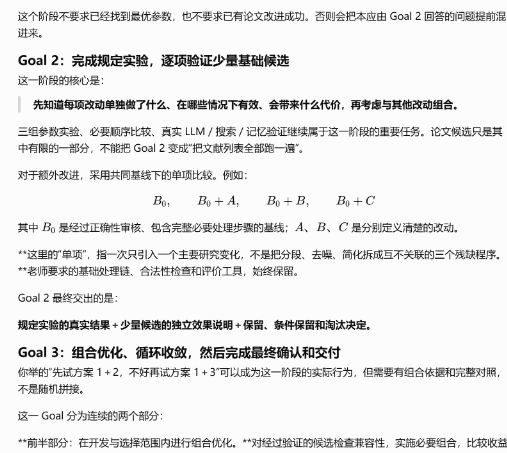
\includegraphics[width=136.500mm]{assets/crops/E07_02_02.png}};
\node[anchor=north west,inner sep=0,text width=36.40mm,align=left] at (159.60,48.51) {\color{Blue}\fontsize{9.5}{13}\selectfont \bfseries 先验证独立改动};
\node[anchor=north west,inner sep=0,text width=36.40mm,align=left] at (159.60,57.16) {\color{Ink}\fontsize{8.7}{12.8}\selectfont  先在可信基线上分别验证少量候选，再考虑组合。这样可以看清每项改动带来的作用和代价，后续组合也有可比较的父方案。};
\draw[draw=Blue,line width=.66pt,rounded corners=1mm,-{Stealth[length=1.8mm,width=1.35mm]}] (157.400,52.009) -- (153.200,52.009) -- (153.200,121.129) -- (42.808,121.129);
\draw[Rule,line width=.35pt] (14,283)--(196,283);
\node[anchor=north west,inner sep=0,text width=170.00mm,align=left] at (14.00,287.00) {\color{Muted}\fontsize{6.7}{8.5}\selectfont  智慧城市与位置服务  /  实验一过程报告  /  Part II};
\node[anchor=north west,inner sep=0,text width=11.00mm,align=left] at (185.00,286.50) {\color{Muted}\fontsize{8}{9}\selectfont  32};
\PageEnd

\PageStart
\node[anchor=north west,inner sep=0,text width=182.00mm,align=left] at (14.00,11.00) {\color{Blue}\fontsize{7.8}{10}\selectfont \bfseries PART II · 实验一中的交互与决策  /  执行与审核机制的落地和修正};
\node[anchor=north west,inner sep=0,text width=182.00mm,align=left] at (14.00,22.00) {\color{Ink}\fontsize{17.5}{22.5}\selectfont \bfseries 用三个Goal组织连续推进（续）};
\node[anchor=north west,inner sep=0,text width=182.00mm,align=left] at (14.00,33.51) {\color{Muted}\fontsize{8.2}{11}\selectfont  接前页，继续阅读这组对话。};
\node[anchor=north west,inner sep=0,text width=136.50mm,align=left] at (14.00,42.51) {\color{Muted}\fontsize{7.2}{9.5}\selectfont  同一回答：单项验证、组合与收敛 · 续页};
\node[anchor=north west,inner sep=0] at (14.000,46.709) {
\includegraphics[width=136.500mm]{assets/crops/E07_03_01.png}};
\node[anchor=north west,inner sep=0,text width=136.50mm,align=left] at (14.00,69.41) {\color{Muted}\fontsize{7.2}{9.5}\selectfont  同一轮：共同评价与专项审核};
\node[anchor=north west,inner sep=0] at (14.000,73.609) {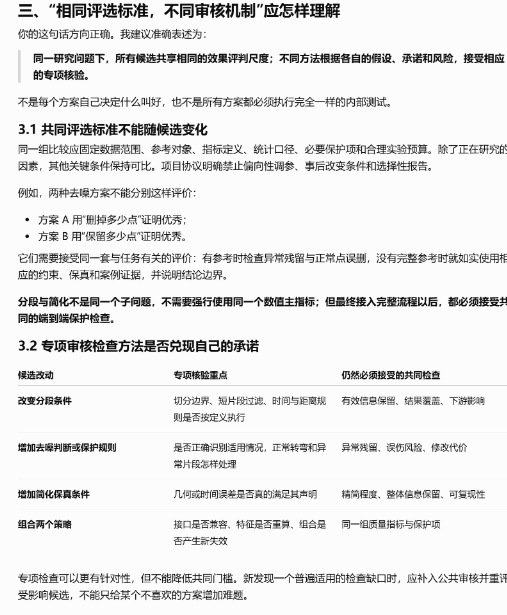
\includegraphics[width=136.500mm]{assets/crops/E07_03_02.png}};
\node[anchor=north west,inner sep=0,text width=36.40mm,align=left] at (159.60,48.51) {\color{Blue}\fontsize{9.5}{13}\selectfont \bfseries 共同评价配合专项核验};
\node[anchor=north west,inner sep=0,text width=36.40mm,align=left] at (159.60,57.16) {\color{Ink}\fontsize{8.7}{12.8}\selectfont  候选共享效果与保护条件；分段、方向处理和DP则分别检查自己的定义与承诺。};
\draw[draw=Blue,line width=.66pt,rounded corners=1mm,-{Stealth[length=1.8mm,width=1.35mm]}] (157.400,52.009) -- (153.200,52.009) -- (153.200,89.090) -- (149.692,89.090);
\node[anchor=north west,inner sep=0,text width=36.40mm,align=left] at (159.60,89.74) {\color{Rose}\fontsize{8.9}{12.5}\selectfont \bfseries 我的回看};
\node[anchor=north west,inner sep=0,text width=36.40mm,align=left] at (159.60,96.74) {\color{Ink}\fontsize{8.5}{12.7}\selectfont  有效的比较会留下采用、保留或淘汰的依据。后续任务接着这些结果推进，负结果也保留下来。};
\draw[Rule,line width=.35pt] (14,283)--(196,283);
\node[anchor=north west,inner sep=0,text width=170.00mm,align=left] at (14.00,287.00) {\color{Muted}\fontsize{6.7}{8.5}\selectfont  智慧城市与位置服务  /  实验一过程报告  /  Part II};
\node[anchor=north west,inner sep=0,text width=11.00mm,align=left] at (185.00,286.50) {\color{Muted}\fontsize{8}{9}\selectfont  33};
\PageEnd

\PageStart
\node[anchor=north west,inner sep=0,text width=182.00mm,align=left] at (14.00,11.00) {\color{Blue}\fontsize{7.8}{10}\selectfont \bfseries PART II · 实验一中的交互与决策  /  执行与审核机制的落地和修正  /  关系图};
\node[anchor=north west,inner sep=0,text width=182.00mm,align=left] at (14.00,25.00) {\color{Ink}\fontsize{18}{24}\selectfont \bfseries 共同评价与专项核验怎样配合};
\node[anchor=north west,inner sep=0,text width=182.00mm,align=left] at (14.00,43.00) {\color{Ink}\fontsize{9.6}{15}\selectfont  各方法分别检查自己的实现，同时在相同原始参考和保护条件下比较结果。};
\node[anchor=north west,inner sep=0] at (14,71) {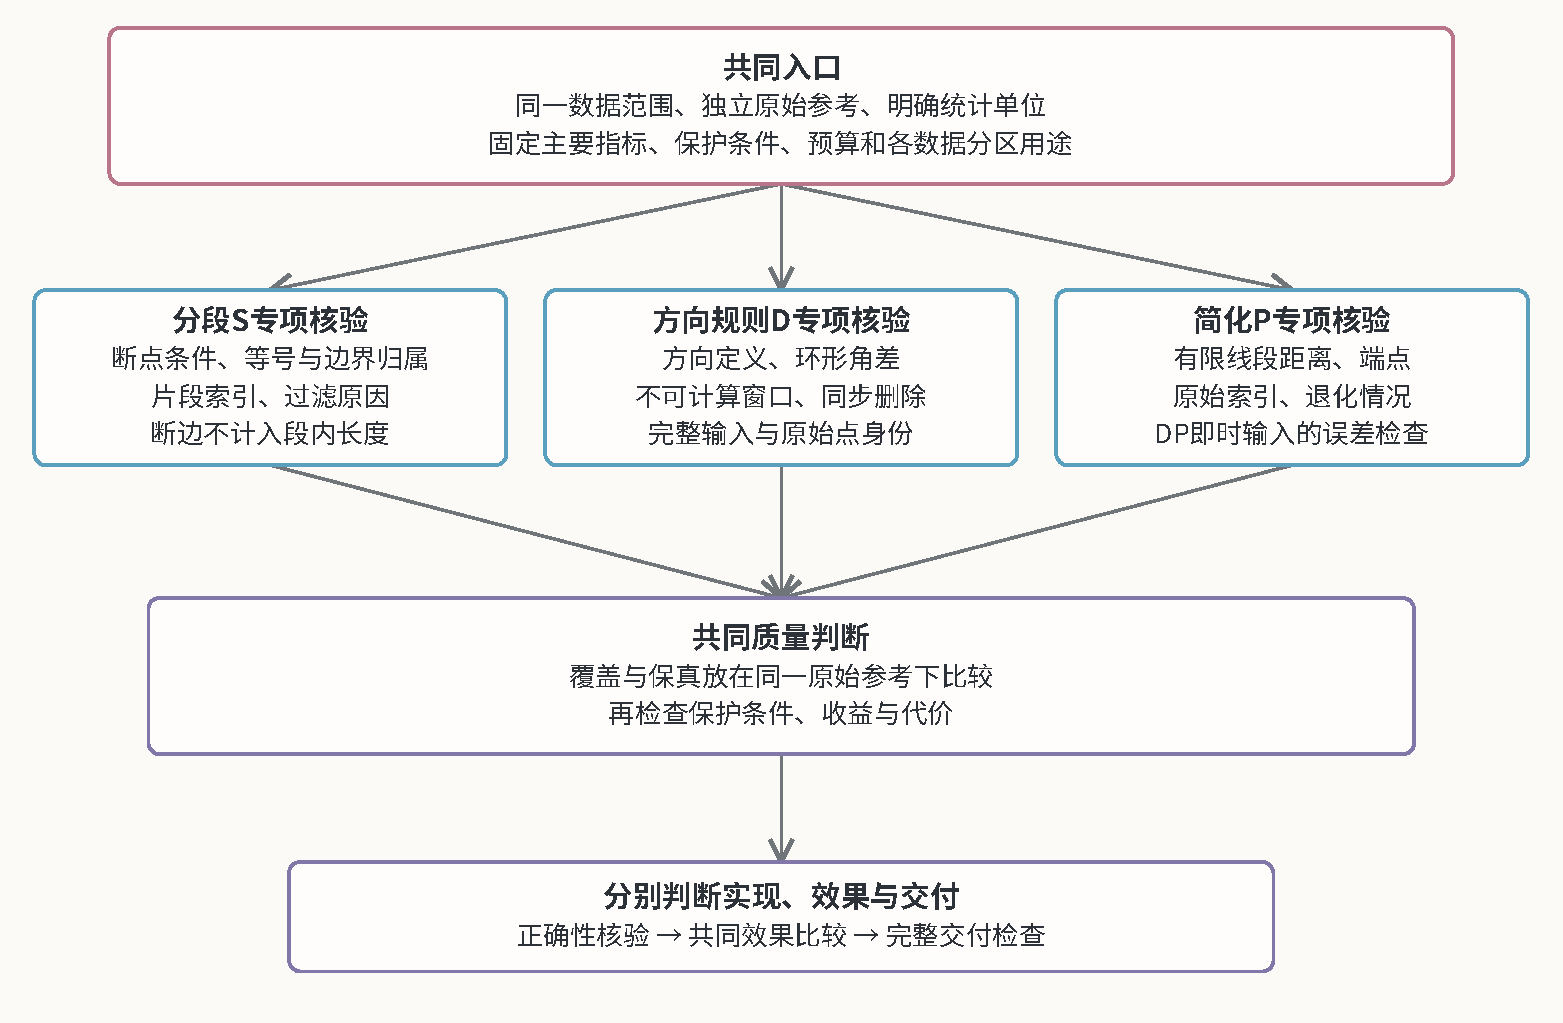
\includegraphics[width=182mm]{figures/D03.pdf}};
\node[anchor=north west,inner sep=0,text width=182.00mm,align=left] at (14.00,200.21) {\color{Ink}\fontsize{10}{15.5}\selectfont  分段、方向规则和简化各有专项检查。进入效果比较后，覆盖、几何偏差和保留情况回到同一原始参考，形成可比较的采用依据。};
\draw[Rule,line width=.35pt] (14,283)--(196,283);
\node[anchor=north west,inner sep=0,text width=170.00mm,align=left] at (14.00,287.00) {\color{Muted}\fontsize{6.7}{8.5}\selectfont  智慧城市与位置服务  /  实验一过程报告  /  Part II};
\node[anchor=north west,inner sep=0,text width=11.00mm,align=left] at (185.00,286.50) {\color{Muted}\fontsize{8}{9}\selectfont  34};
\PageEnd

\PageStart
\node[anchor=north west,inner sep=0,text width=182.00mm,align=left] at (14.00,11.00) {\color{Blue}\fontsize{7.8}{10}\selectfont \bfseries PART II · 实验一中的交互与决策  /  执行与审核机制的落地和修正};
\node[anchor=north west,inner sep=0,text width=182.00mm,align=left] at (14.00,22.00) {\color{Ink}\fontsize{17.5}{22.5}\selectfont \bfseries 第一次核验发现：包装层改变了检查对象};
\node[anchor=north west,inner sep=0,text width=182.00mm,align=left] at (14.00,33.51) {\color{Ink}\fontsize{9.5}{14.6}\selectfont  我把提示词交给 Codex，再把回复和仓库交给 GPT 检查。第一次审核追到了工具包装层：错误输入可能在核验前就被改掉，结果错误列表也被放行。};
\node[anchor=north west,inner sep=0] at (14,8) {\hypertarget{E08}{}};
\node[anchor=north west,inner sep=0,text width=136.50mm,align=left] at (14.00,48.63) {\color{Muted}\fontsize{7.2}{9.5}\selectfont  我批准执行并要求真实远程检查};
\node[anchor=north west,inner sep=0] at (14.000,52.828) {
\includegraphics[width=136.500mm]{assets/crops/E08_01_01.png}};
\node[anchor=north west,inner sep=0,text width=136.50mm,align=left] at (14.00,107.39) {\color{Muted}\fontsize{7.2}{9.5}\selectfont  工程返回后的首次审核结论};
\node[anchor=north west,inner sep=0] at (14.000,111.595) {
\includegraphics[width=136.500mm]{assets/crops/E08_01_02.png}};
\node[anchor=north west,inner sep=0,text width=36.40mm,align=left] at (159.60,54.63) {\color{Blue}\fontsize{9.5}{13}\selectfont \bfseries 保留进展，继续追查问题};
\node[anchor=north west,inner sep=0,text width=36.40mm,align=left] at (159.60,67.86) {\color{Ink}\fontsize{8.7}{12.8}\selectfont  材料保护、诊断和几何工具已有进展。GPT在此基础上继续检查审核器，把新发现的漏洞交回修复。};
\draw[draw=Blue,line width=.66pt,rounded corners=1mm,-{Stealth[length=1.8mm,width=1.35mm]}] (157.400,58.128) -- (153.200,58.128) -- (153.200,72.116) -- (114.891,72.116);
\draw[Rule,line width=.35pt] (14,283)--(196,283);
\node[anchor=north west,inner sep=0,text width=170.00mm,align=left] at (14.00,287.00) {\color{Muted}\fontsize{6.7}{8.5}\selectfont  智慧城市与位置服务  /  实验一过程报告  /  Part II};
\node[anchor=north west,inner sep=0,text width=11.00mm,align=left] at (185.00,286.50) {\color{Muted}\fontsize{8}{9}\selectfont  35};
\PageEnd

\PageStart
\node[anchor=north west,inner sep=0,text width=182.00mm,align=left] at (14.00,11.00) {\color{Blue}\fontsize{7.8}{10}\selectfont \bfseries PART II · 实验一中的交互与决策  /  执行与审核机制的落地和修正};
\node[anchor=north west,inner sep=0,text width=182.00mm,align=left] at (14.00,22.00) {\color{Ink}\fontsize{17.5}{22.5}\selectfont \bfseries 第一次核验发现：包装层改变了检查对象（续）};
\node[anchor=north west,inner sep=0,text width=182.00mm,align=left] at (14.00,33.51) {\color{Muted}\fontsize{8.2}{11}\selectfont  接前页，继续阅读这组对话。};
\node[anchor=north west,inner sep=0,text width=136.50mm,align=left] at (14.00,42.51) {\color{Muted}\fontsize{7.2}{9.5}\selectfont  同一轮：包装层让错误列表通过};
\node[anchor=north west,inner sep=0] at (14.000,46.709) {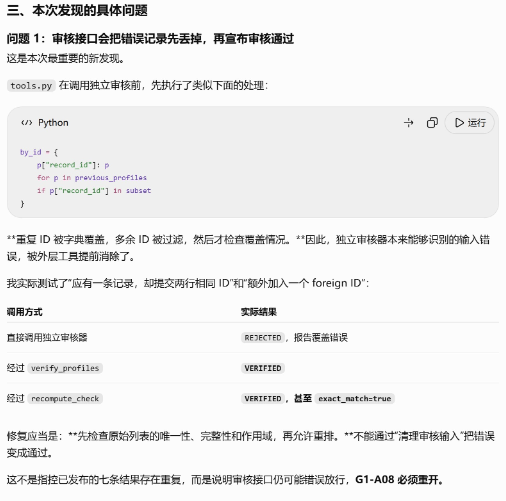
\includegraphics[width=136.500mm]{assets/crops/E08_02_01.png}};
\node[anchor=north west,inner sep=0,text width=36.40mm,align=left] at (159.60,48.51) {\color{Blue}\fontsize{9.5}{13}\selectfont \bfseries 先检查原始提交};
\node[anchor=north west,inner sep=0,text width=36.40mm,align=left] at (159.60,57.16) {\color{Ink}\fontsize{8.7}{12.8}\selectfont  重复ID被覆盖、额外ID被过滤后，错误输入会看起来完整。修复需要把唯一性和范围检查放在这些处理之前。};
\draw[draw=Blue,line width=.66pt,rounded corners=1mm,-{Stealth[length=1.8mm,width=1.35mm]}] (157.400,52.009) -- (153.200,52.009) -- (153.200,154.075) -- (120.556,154.075);
\draw[Rule,line width=.35pt] (14,283)--(196,283);
\node[anchor=north west,inner sep=0,text width=170.00mm,align=left] at (14.00,287.00) {\color{Muted}\fontsize{6.7}{8.5}\selectfont  智慧城市与位置服务  /  实验一过程报告  /  Part II};
\node[anchor=north west,inner sep=0,text width=11.00mm,align=left] at (185.00,286.50) {\color{Muted}\fontsize{8}{9}\selectfont  36};
\PageEnd

\PageStart
\node[anchor=north west,inner sep=0,text width=182.00mm,align=left] at (14.00,11.00) {\color{Blue}\fontsize{7.8}{10}\selectfont \bfseries PART II · 实验一中的交互与决策  /  执行与审核机制的落地和修正};
\node[anchor=north west,inner sep=0,text width=182.00mm,align=left] at (14.00,22.00) {\color{Ink}\fontsize{17.5}{22.5}\selectfont \bfseries 把独立参考接到真正需要核验的产物上};
\node[anchor=north west,inner sep=0,text width=182.00mm,align=left] at (14.00,33.51) {\color{Ink}\fontsize{9.5}{14.6}\selectfont  列表问题修好后，我继续转交结果。GPT的新检查发现两个缺口：请求检查的产物没有真正进入核验；baseline又把候选自己的输入、参数和账本当成独立参考。};
\node[anchor=north west,inner sep=0] at (14,8) {\hypertarget{E09}{}};
\node[anchor=north west,inner sep=0,text width=136.50mm,align=left] at (14.00,48.63) {\color{Muted}\fontsize{7.2}{9.5}\selectfont  我转交的Codex阶段回复};
\node[anchor=north west,inner sep=0] at (14.000,52.828) {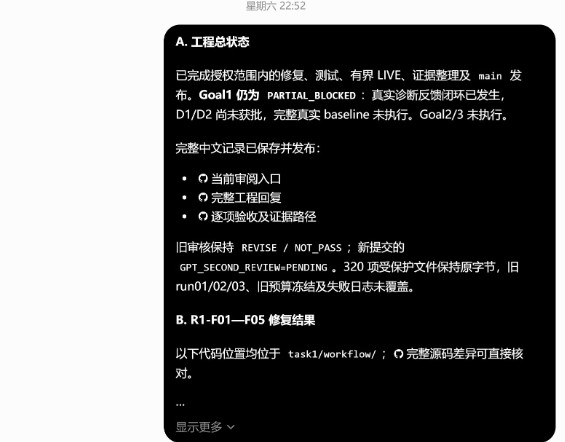
\includegraphics[width=136.500mm]{assets/crops/E09_01_01.png}};
\node[anchor=north west,inner sep=0,text width=136.50mm,align=left] at (14.00,164.81) {\color{Muted}\fontsize{7.2}{9.5}\selectfont  GPT发现核验范围与请求不一致};
\node[anchor=north west,inner sep=0] at (14.000,169.012) {
\includegraphics[width=136.500mm]{assets/crops/E09_01_02.png}};
\node[anchor=north west,inner sep=0,text width=36.40mm,align=left] at (159.60,54.63) {\color{Blue}\fontsize{9.5}{13}\selectfont \bfseries 我转交结果，GPT继续检查};
\node[anchor=north west,inner sep=0,text width=36.40mm,align=left] at (159.60,67.86) {\color{Ink}\fontsize{8.7}{12.8}\selectfont  我把Codex的阶段回执和仓库交给GPT。新的核验继续追到产物范围及参考来源，找出了此前未覆盖的问题。};
\draw[draw=Blue,line width=.66pt,rounded corners=1mm,-{Stealth[length=1.8mm,width=1.35mm]}] (157.400,58.128) -- (153.200,58.128) -- (153.200,80.491) -- (137.212,80.491);
\draw[Rule,line width=.35pt] (14,283)--(196,283);
\node[anchor=north west,inner sep=0,text width=170.00mm,align=left] at (14.00,287.00) {\color{Muted}\fontsize{6.7}{8.5}\selectfont  智慧城市与位置服务  /  实验一过程报告  /  Part II};
\node[anchor=north west,inner sep=0,text width=11.00mm,align=left] at (185.00,286.50) {\color{Muted}\fontsize{8}{9}\selectfont  37};
\PageEnd

\PageStart
\node[anchor=north west,inner sep=0,text width=182.00mm,align=left] at (14.00,11.00) {\color{Blue}\fontsize{7.8}{10}\selectfont \bfseries PART II · 实验一中的交互与决策  /  执行与审核机制的落地和修正};
\node[anchor=north west,inner sep=0,text width=182.00mm,align=left] at (14.00,22.00) {\color{Ink}\fontsize{17.5}{22.5}\selectfont \bfseries 把独立参考接到真正需要核验的产物上（续）};
\node[anchor=north west,inner sep=0,text width=182.00mm,align=left] at (14.00,33.51) {\color{Muted}\fontsize{8.2}{11}\selectfont  接前页，继续阅读这组对话。};
\node[anchor=north west,inner sep=0,text width=136.50mm,align=left] at (14.00,42.51) {\color{Muted}\fontsize{7.2}{9.5}\selectfont  GPT发现核验范围与请求不一致 · 续页};
\node[anchor=north west,inner sep=0] at (14.000,46.709) {
\includegraphics[width=136.500mm]{assets/crops/E09_02_01.png}};
\node[anchor=north west,inner sep=0,text width=136.50mm,align=left] at (14.00,92.01) {\color{Muted}\fontsize{7.2}{9.5}\selectfont  同一轮：候选自证被反例揭穿};
\node[anchor=north west,inner sep=0] at (14.000,96.214) {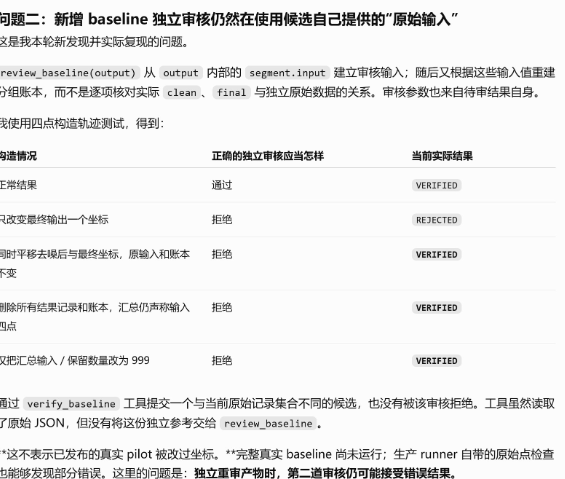
\includegraphics[width=136.500mm]{assets/crops/E09_02_02.png}};
\node[anchor=north west,inner sep=0,text width=36.40mm,align=left] at (159.60,48.51) {\color{Blue}\fontsize{9.5}{13}\selectfont \bfseries 参考要来自候选之外};
\node[anchor=north west,inner sep=0,text width=36.40mm,align=left] at (159.60,57.16) {\color{Ink}\fontsize{8.7}{12.8}\selectfont  时间分区需要对应的检查入口；baseline需要独立绑定原始输入。平移clean和final仍过关的反例暴露了自证问题。};
\draw[draw=Blue,line width=.66pt,rounded corners=1mm,-{Stealth[length=1.8mm,width=1.35mm]}] (157.400,52.009) -- (153.200,52.009) -- (153.200,170.262) -- (125.374,170.262);
\draw[Rule,line width=.35pt] (14,283)--(196,283);
\node[anchor=north west,inner sep=0,text width=170.00mm,align=left] at (14.00,287.00) {\color{Muted}\fontsize{6.7}{8.5}\selectfont  智慧城市与位置服务  /  实验一过程报告  /  Part II};
\node[anchor=north west,inner sep=0,text width=11.00mm,align=left] at (185.00,286.50) {\color{Muted}\fontsize{8}{9}\selectfont  38};
\PageEnd

\PageStart
\node[anchor=north west,inner sep=0,text width=182.00mm,align=left] at (14.00,11.00) {\color{Blue}\fontsize{7.8}{10}\selectfont \bfseries PART II · 实验一中的交互与决策  /  执行与审核机制的落地和修正};
\node[anchor=north west,inner sep=0,text width=182.00mm,align=left] at (14.00,22.00) {\color{Ink}\fontsize{17.5}{22.5}\selectfont \bfseries 把修复和任务恢复留在当前Goal};
\node[anchor=north west,inner sep=0,text width=182.00mm,align=left] at (14.00,33.51) {\color{Ink}\fontsize{9.5}{14.6}\selectfont  几轮交接后，我发现每个普通工程错误都要由我转发下一条修复提示词。我因此要求把修复、回归、重建和恢复原任务都纳入当前Goal，让体系接着处理这些已经定位的问题。};
\node[anchor=north west,inner sep=0] at (14,8) {\hypertarget{E10}{}};
\node[anchor=north west,inner sep=0,text width=136.50mm,align=left] at (14.00,48.63) {\color{Muted}\fontsize{7.2}{9.5}\selectfont  我指出反复外部转发的问题};
\node[anchor=north west,inner sep=0] at (14.000,52.828) {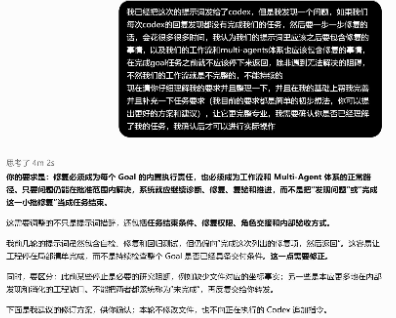
\includegraphics[width=136.500mm]{assets/crops/E10_01_01.png}};
\node[anchor=north west,inner sep=0,text width=136.50mm,align=left] at (14.00,167.64) {\color{Muted}\fontsize{7.2}{9.5}\selectfont  GPT改为对Goal完成负责};
\node[anchor=north west,inner sep=0] at (14.000,171.842) {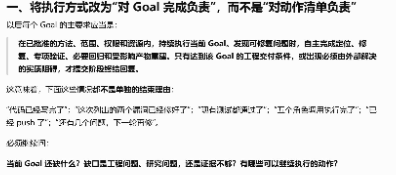
\includegraphics[width=136.500mm]{assets/crops/E10_01_02.png}};
\node[anchor=north west,inner sep=0,text width=36.40mm,align=left] at (159.60,54.63) {\color{Blue}\fontsize{9.5}{13}\selectfont \bfseries 减少反复外部交接};
\node[anchor=north west,inner sep=0,text width=36.40mm,align=left] at (159.60,63.28) {\color{Ink}\fontsize{8.7}{12.8}\selectfont  我希望能够自行定位的普通工程问题由当前执行过程继续解决，把我的参与集中在真正需要判断的研究问题上。};
\draw[draw=Blue,line width=.66pt,rounded corners=1mm,-{Stealth[length=1.8mm,width=1.35mm]}] (157.400,58.128) -- (153.200,58.128) -- (153.200,78.681) -- (112.928,78.681);
\draw[Rule,line width=.35pt] (14,283)--(196,283);
\node[anchor=north west,inner sep=0,text width=170.00mm,align=left] at (14.00,287.00) {\color{Muted}\fontsize{6.7}{8.5}\selectfont  智慧城市与位置服务  /  实验一过程报告  /  Part II};
\node[anchor=north west,inner sep=0,text width=11.00mm,align=left] at (185.00,286.50) {\color{Muted}\fontsize{8}{9}\selectfont  39};
\PageEnd

\PageStart
\node[anchor=north west,inner sep=0,text width=182.00mm,align=left] at (14.00,11.00) {\color{Blue}\fontsize{7.8}{10}\selectfont \bfseries PART II · 实验一中的交互与决策  /  执行与审核机制的落地和修正};
\node[anchor=north west,inner sep=0,text width=182.00mm,align=left] at (14.00,22.00) {\color{Ink}\fontsize{17.5}{22.5}\selectfont \bfseries 把修复和任务恢复留在当前Goal（续）};
\node[anchor=north west,inner sep=0,text width=182.00mm,align=left] at (14.00,33.51) {\color{Muted}\fontsize{8.2}{11}\selectfont  接前页，继续阅读这组对话。};
\node[anchor=north west,inner sep=0,text width=136.50mm,align=left] at (14.00,42.51) {\color{Muted}\fontsize{7.2}{9.5}\selectfont  GPT改为对Goal完成负责 · 续页};
\node[anchor=north west,inner sep=0] at (14.000,46.709) {
\includegraphics[width=136.500mm]{assets/crops/E10_02_01.png}};
\node[anchor=north west,inner sep=0,text width=136.50mm,align=left] at (14.00,78.80) {\color{Muted}\fontsize{7.2}{9.5}\selectfont  后续明确B-Repair与恢复原任务};
\node[anchor=north west,inner sep=0] at (14.000,82.996) {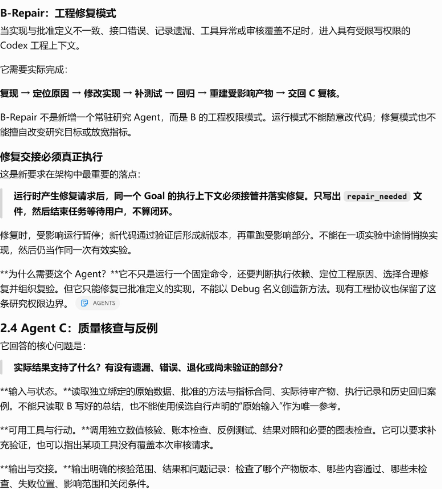
\includegraphics[width=136.500mm]{assets/crops/E10_02_02.png}};
\node[anchor=north west,inner sep=0,text width=36.40mm,align=left] at (159.60,48.51) {\color{Blue}\fontsize{9.5}{13}\selectfont \bfseries 修复后接着完成原任务};
\node[anchor=north west,inner sep=0,text width=36.40mm,align=left] at (159.60,57.16) {\color{Ink}\fontsize{8.7}{12.8}\selectfont  GPT把B-Repair明确为执行角色的修复模式：实际修正、重跑受影响结果，经C复验，再恢复父任务。};
\draw[draw=Blue,line width=.66pt,rounded corners=1mm,-{Stealth[length=1.8mm,width=1.35mm]}] (157.400,52.009) -- (153.200,52.009) -- (153.200,176.569) -- (50.750,176.569);
\node[anchor=north west,inner sep=0,text width=36.40mm,align=left] at (159.60,94.25) {\color{Rose}\fontsize{8.9}{12.5}\selectfont \bfseries 我的回看};
\node[anchor=north west,inner sep=0,text width=36.40mm,align=left] at (159.60,101.25) {\color{Ink}\fontsize{8.5}{12.7}\selectfont  早期由我多次转发修复提示词，后来才逐步形成内部接管。这次反馈改变了任务的停止条件。};
\draw[Rule,line width=.35pt] (14,283)--(196,283);
\node[anchor=north west,inner sep=0,text width=170.00mm,align=left] at (14.00,287.00) {\color{Muted}\fontsize{6.7}{8.5}\selectfont  智慧城市与位置服务  /  实验一过程报告  /  Part II};
\node[anchor=north west,inner sep=0,text width=11.00mm,align=left] at (185.00,286.50) {\color{Muted}\fontsize{8}{9}\selectfont  40};
\PageEnd

\PageStart
\node[anchor=north west,inner sep=0,text width=182.00mm,align=left] at (14.00,11.00) {\color{Blue}\fontsize{7.8}{10}\selectfont \bfseries PART II · 实验一中的交互与决策  /  执行与审核机制的落地和修正  /  关系图};
\node[anchor=north west,inner sep=0,text width=182.00mm,align=left] at (14.00,25.00) {\color{Ink}\fontsize{18}{24}\selectfont \bfseries 研究优化与工程修复分别怎样继续};
\node[anchor=north west,inner sep=0,text width=182.00mm,align=left] at (14.00,43.00) {\color{Ink}\fontsize{9.6}{15}\selectfont  早期由我转发修复提示词；在我的反馈后，普通工程问题逐步改为在当前Goal内修复和恢复。};
\node[anchor=north west,inner sep=0] at (14,71) {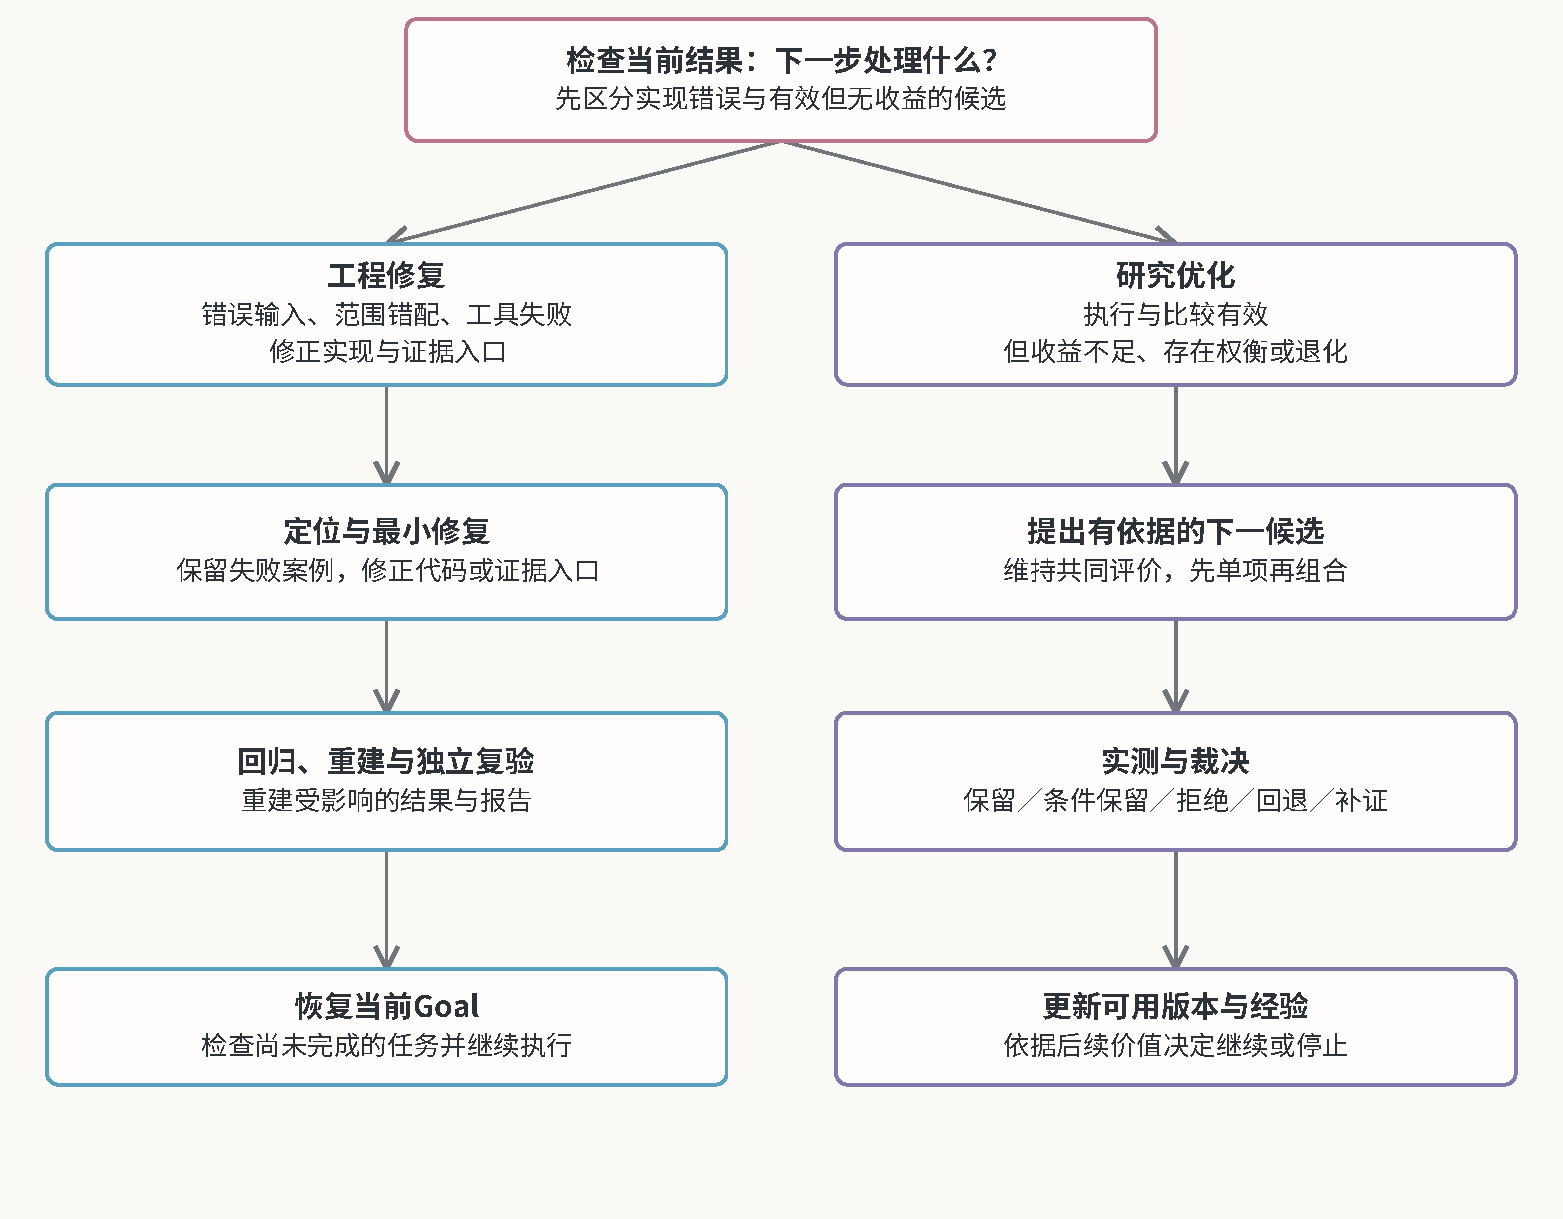
\includegraphics[width=182mm]{figures/D02.pdf}};
\node[anchor=north west,inner sep=0,text width=182.00mm,align=left] at (14.00,222.96) {\color{Ink}\fontsize{10}{15.5}\selectfont  左侧修正偏离既定定义的实现，经过回归和复验恢复任务；右侧检验有效候选的作用，按比较结果决定保留、回退、补证或停止。};
\draw[Rule,line width=.35pt] (14,283)--(196,283);
\node[anchor=north west,inner sep=0,text width=170.00mm,align=left] at (14.00,287.00) {\color{Muted}\fontsize{6.7}{8.5}\selectfont  智慧城市与位置服务  /  实验一过程报告  /  Part II};
\node[anchor=north west,inner sep=0,text width=11.00mm,align=left] at (185.00,286.50) {\color{Muted}\fontsize{8}{9}\selectfont  41};
\PageEnd

\PageStart
\node[anchor=north west,inner sep=0,text width=182.00mm,align=left] at (14.00,11.00) {\color{Blue}\fontsize{7.8}{10}\selectfont \bfseries PART II · 实验一中的交互与决策  /  执行与审核机制的落地和修正};
\node[anchor=north west,inner sep=0,text width=182.00mm,align=left] at (14.00,22.00) {\color{Ink}\fontsize{17.5}{22.5}\selectfont \bfseries 用正反例和真实试运行检验修复结果};
\node[anchor=north west,inner sep=0,text width=182.00mm,align=left] at (14.00,33.51) {\color{Ink}\fontsize{9.5}{14.6}\selectfont  我前面已要求在当前Goal内继续修复。随后交付的结果让这项要求可以被实际检查：关键漏洞通过正反例回归，七条试运行记录也得到了可独立复算的处理结果。};
\node[anchor=north west,inner sep=0] at (14,8) {\hypertarget{E11}{}};
\node[anchor=north west,inner sep=0,text width=136.50mm,align=left] at (14.00,48.63) {\color{Muted}\fontsize{7.2}{9.5}\selectfont  回引前期要求：在当前Goal内继续修复};
\node[anchor=north west,inner sep=0] at (14.000,52.828) {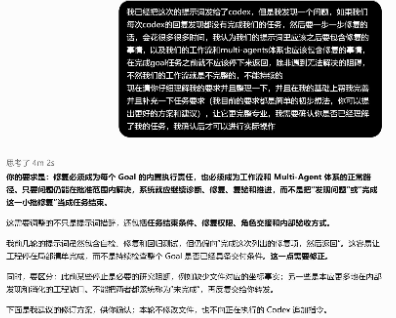
\includegraphics[width=136.500mm]{assets/crops/E11_01_01.png}};
\node[anchor=north west,inner sep=0,text width=136.50mm,align=left] at (14.00,167.64) {\color{Muted}\fontsize{7.2}{9.5}\selectfont  后续：Goal 1限定范围内通过};
\node[anchor=north west,inner sep=0] at (14.000,171.842) {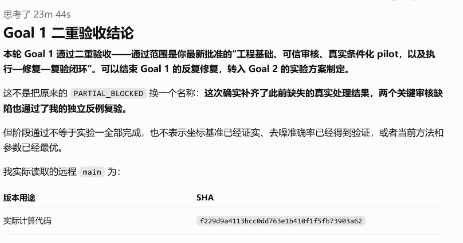
\includegraphics[width=136.500mm]{assets/crops/E11_01_02.png}};
\node[anchor=north west,inner sep=0,text width=36.40mm,align=left] at (159.60,54.63) {\color{Blue}\fontsize{9.5}{13}\selectfont \bfseries 可信基线开始形成};
\node[anchor=north west,inner sep=0,text width=36.40mm,align=left] at (159.60,63.28) {\color{Ink}\fontsize{8.7}{12.8}\selectfont  七条试运行记录把实际处理、输出检查、修复和复验接了起来，为后续参数与方法比较提供了基础。};
\draw[draw=Blue,line width=.66pt,rounded corners=1mm,-{Stealth[length=1.8mm,width=1.35mm]}] (157.400,58.128) -- (153.200,58.128) -- (153.200,78.681) -- (112.928,78.681);
\draw[Rule,line width=.35pt] (14,283)--(196,283);
\node[anchor=north west,inner sep=0,text width=170.00mm,align=left] at (14.00,287.00) {\color{Muted}\fontsize{6.7}{8.5}\selectfont  智慧城市与位置服务  /  实验一过程报告  /  Part II};
\node[anchor=north west,inner sep=0,text width=11.00mm,align=left] at (185.00,286.50) {\color{Muted}\fontsize{8}{9}\selectfont  42};
\PageEnd

\PageStart
\node[anchor=north west,inner sep=0,text width=182.00mm,align=left] at (14.00,11.00) {\color{Blue}\fontsize{7.8}{10}\selectfont \bfseries PART II · 实验一中的交互与决策  /  执行与审核机制的落地和修正};
\node[anchor=north west,inner sep=0,text width=182.00mm,align=left] at (14.00,22.00) {\color{Ink}\fontsize{17.5}{22.5}\selectfont \bfseries 用正反例和真实试运行检验修复结果（续）};
\node[anchor=north west,inner sep=0,text width=182.00mm,align=left] at (14.00,33.51) {\color{Muted}\fontsize{8.2}{11}\selectfont  接前页，继续阅读这组对话。};
\node[anchor=north west,inner sep=0,text width=136.50mm,align=left] at (14.00,42.51) {\color{Muted}\fontsize{7.2}{9.5}\selectfont  关键审核反例的关闭记录};
\node[anchor=north west,inner sep=0] at (14.000,46.709) {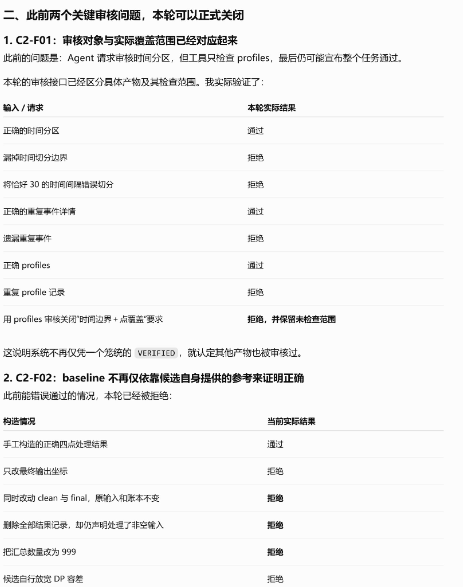
\includegraphics[width=136.500mm]{assets/crops/E11_02_01.png}};
\node[anchor=north west,inner sep=0,text width=36.40mm,align=left] at (159.60,48.51) {\color{Blue}\fontsize{9.5}{13}\selectfont \bfseries 核验对象要逐项对应};
\node[anchor=north west,inner sep=0,text width=36.40mm,align=left] at (159.60,57.16) {\color{Ink}\fontsize{8.7}{12.8}\selectfont  新的检查分别覆盖时间切分、重复事件、原始输入和点数账本。正常输入通过，错分、缺失、错误版本和候选自证都有对应的拒绝结果。};
\draw[Rule,line width=.35pt] (14,283)--(196,283);
\node[anchor=north west,inner sep=0,text width=170.00mm,align=left] at (14.00,287.00) {\color{Muted}\fontsize{6.7}{8.5}\selectfont  智慧城市与位置服务  /  实验一过程报告  /  Part II};
\node[anchor=north west,inner sep=0,text width=11.00mm,align=left] at (185.00,286.50) {\color{Muted}\fontsize{8}{9}\selectfont  43};
\PageEnd

\PageStart
\node[anchor=north west,inner sep=0,text width=182.00mm,align=left] at (14.00,11.00) {\color{Blue}\fontsize{7.8}{10}\selectfont \bfseries PART II · 实验一中的交互与决策  /  执行与审核机制的落地和修正};
\node[anchor=north west,inner sep=0,text width=182.00mm,align=left] at (14.00,22.00) {\color{Ink}\fontsize{17.5}{22.5}\selectfont \bfseries 用正反例和真实试运行检验修复结果（续）};
\node[anchor=north west,inner sep=0,text width=182.00mm,align=left] at (14.00,33.51) {\color{Muted}\fontsize{8.2}{11}\selectfont  接前页，继续阅读这组对话。};
\node[anchor=north west,inner sep=0,text width=136.50mm,align=left] at (14.00,42.51) {\color{Muted}\fontsize{7.2}{9.5}\selectfont  关键审核反例的关闭记录 · 续页};
\node[anchor=north west,inner sep=0] at (14.000,46.709) {
\includegraphics[width=136.500mm]{assets/crops/E11_03_01.png}};
\node[anchor=north west,inner sep=0,text width=136.50mm,align=left] at (14.00,96.43) {\color{Muted}\fontsize{7.2}{9.5}\selectfont  同一轮：修复、复验和任务恢复};
\node[anchor=north west,inner sep=0] at (14.000,100.627) {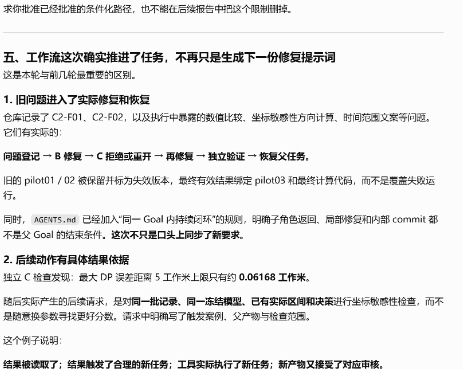
\includegraphics[width=136.500mm]{assets/crops/E11_03_02.png}};
\node[anchor=north west,inner sep=0,text width=36.40mm,align=left] at (159.60,48.51) {\color{Blue}\fontsize{9.5}{13}\selectfont \bfseries 正例与反例一起回归};
\node[anchor=north west,inner sep=0,text width=36.40mm,align=left] at (159.60,57.16) {\color{Ink}\fontsize{8.7}{12.8}\selectfont  正确输入仍能通过，旧漏洞有对应的拒绝测试。七条已经用于检查的记录，随后保留为开发和回归材料。};
\draw[draw=Blue,line width=.66pt,rounded corners=1mm,-{Stealth[length=1.8mm,width=1.35mm]}] (157.400,52.009) -- (153.200,52.009) -- (153.200,129.813) -- (59.402,129.813);
\node[anchor=north west,inner sep=0,text width=36.40mm,align=left] at (159.60,94.25) {\color{Rose}\fontsize{8.9}{12.5}\selectfont \bfseries 我的回看};
\node[anchor=north west,inner sep=0,text width=36.40mm,align=left] at (159.60,101.25) {\color{Ink}\fontsize{8.5}{12.7}\selectfont  坐标来源与计算模型继续分开记录。基线建立后，下一阶段再比较参数、顺序和处理效果。};
\draw[Rule,line width=.35pt] (14,283)--(196,283);
\node[anchor=north west,inner sep=0,text width=170.00mm,align=left] at (14.00,287.00) {\color{Muted}\fontsize{6.7}{8.5}\selectfont  智慧城市与位置服务  /  实验一过程报告  /  Part II};
\node[anchor=north west,inner sep=0,text width=11.00mm,align=left] at (185.00,286.50) {\color{Muted}\fontsize{8}{9}\selectfont  44};
\PageEnd

\PageStart
\node[anchor=north west,inner sep=0,text width=182.00mm,align=left] at (14.00,11.00) {\color{Blue}\fontsize{7.8}{10}\selectfont \bfseries PART II · 实验一中的交互与决策  /  执行与审核机制的落地和修正  /  关系图};
\node[anchor=north west,inner sep=0,text width=182.00mm,align=left] at (14.00,25.00) {\color{Ink}\fontsize{18}{24}\selectfont \bfseries 任务、判断职责与确定性工具};
\node[anchor=north west,inner sep=0,text width=182.00mm,align=left] at (14.00,43.00) {\color{Ink}\fontsize{9.6}{15}\selectfont  我与GPT先明确研究原则，再由诊断、执行和核验角色配合确定性工具完成任务。};
\node[anchor=north west,inner sep=0] at (14,71) {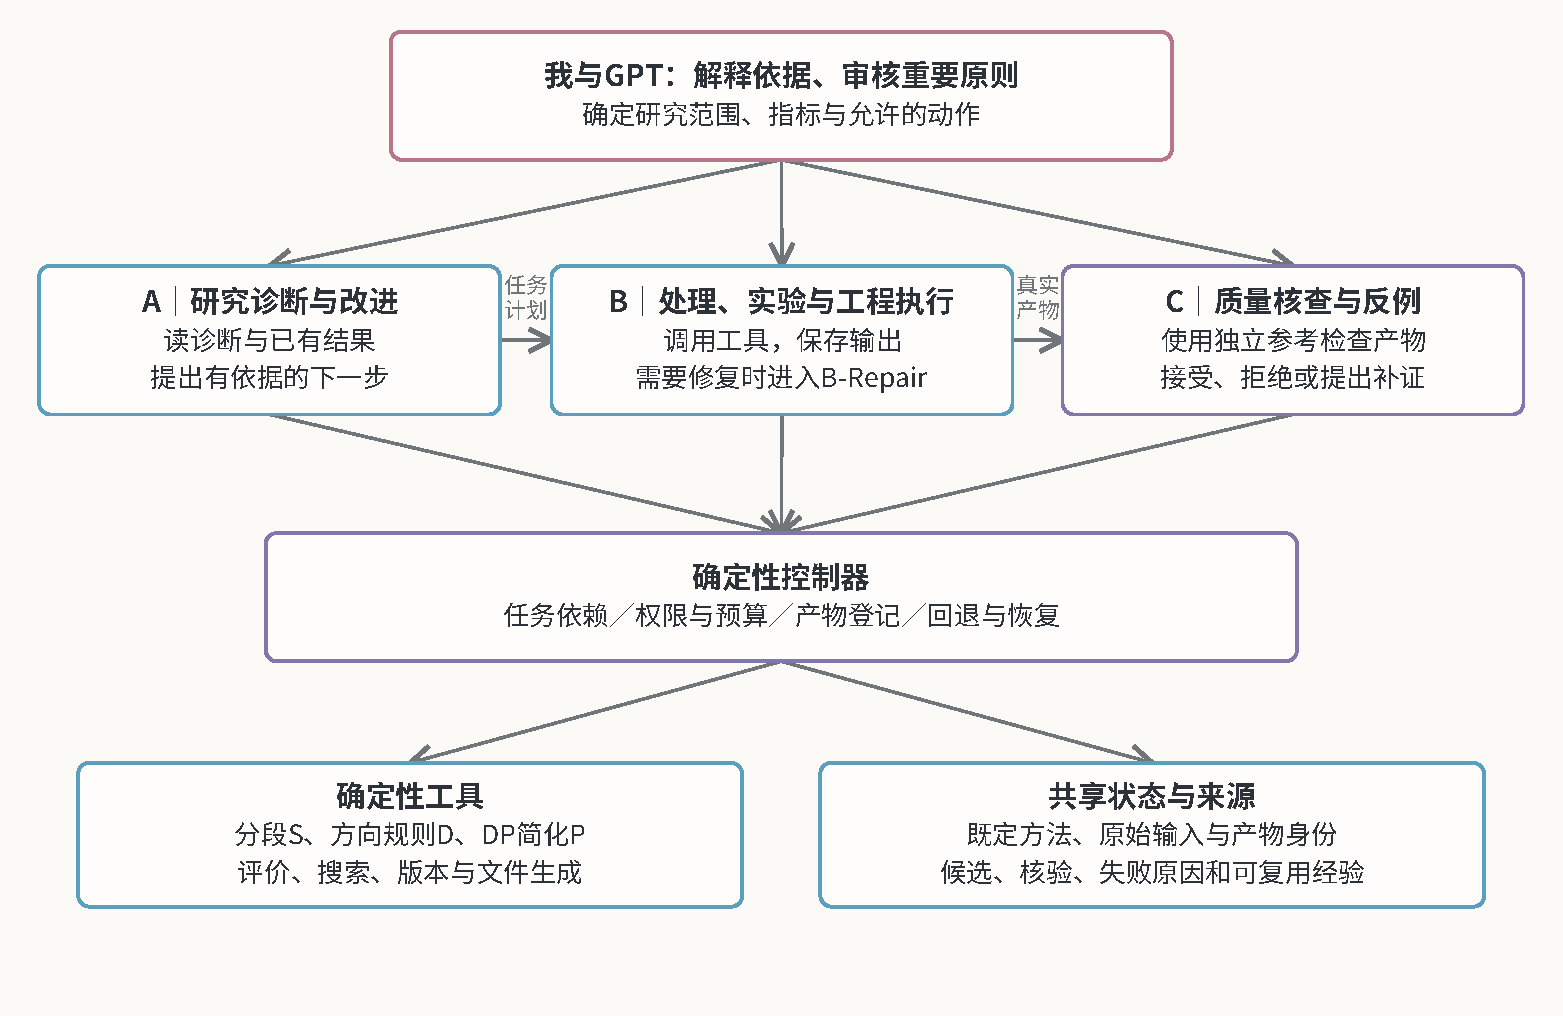
\includegraphics[width=182mm]{figures/D01.pdf}};
\node[anchor=north west,inner sep=0,text width=182.00mm,align=left] at (14.00,199.30) {\color{Ink}\fontsize{10}{15.5}\selectfont  任务计划、实际产物和核验结果在角色之间传递；控制器管理依赖、预算和恢复，共享状态保存相应的输入、输出与判断依据。};
\draw[Rule,line width=.35pt] (14,283)--(196,283);
\node[anchor=north west,inner sep=0,text width=170.00mm,align=left] at (14.00,287.00) {\color{Muted}\fontsize{6.7}{8.5}\selectfont  智慧城市与位置服务  /  实验一过程报告  /  Part II};
\node[anchor=north west,inner sep=0,text width=11.00mm,align=left] at (185.00,286.50) {\color{Muted}\fontsize{8}{9}\selectfont  45};
\PageEnd

\PageStart
\node[anchor=north west,inner sep=0,text width=182.00mm,align=left] at (14.00,11.00) {\color{Blue}\fontsize{7.8}{10}\selectfont \bfseries PART II · 实验一中的交互与决策  /  共同评价下的实验与AI建议检验};
\node[anchor=north west,inner sep=0,text width=182.00mm,align=left] at (14.00,22.00) {\color{Ink}\fontsize{17.5}{22.5}\selectfont \bfseries 先确定比较条件，再开展参数实验};
\node[anchor=north west,inner sep=0,text width=182.00mm,align=left] at (14.00,33.51) {\color{Ink}\fontsize{9.5}{14.6}\selectfont  进入Goal 2前，我要求在原体系中完成规定实验、共同评价和持续修复。结果回来时，GPT先核对实际运行的配置、开发与评价数据的用途，再分析不同设置带来的变化。};
\node[anchor=north west,inner sep=0] at (14,8) {\hypertarget{E12}{}};
\node[anchor=north west,inner sep=0,text width=136.50mm,align=left] at (14.00,48.63) {\color{Muted}\fontsize{7.2}{9.5}\selectfont  我要求在原体系中完成Goal 2};
\node[anchor=north west,inner sep=0] at (14.000,52.828) {
\includegraphics[width=136.500mm]{assets/crops/E12_01_01.png}};
\node[anchor=north west,inner sep=0,text width=136.50mm,align=left] at (14.00,121.41) {\color{Muted}\fontsize{7.2}{9.5}\selectfont  完成后的审核：数据用途与覆盖};
\node[anchor=north west,inner sep=0] at (14.000,125.614) {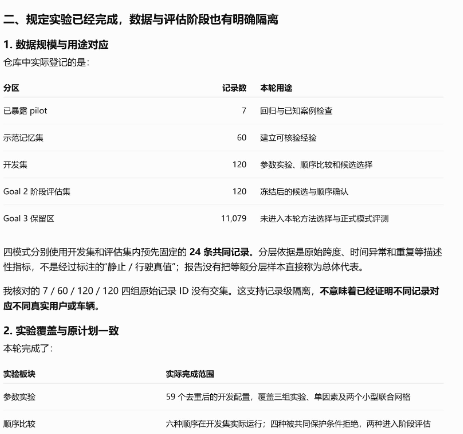
\includegraphics[width=136.500mm]{assets/crops/E12_01_02.png}};
\node[anchor=north west,inner sep=0,text width=36.40mm,align=left] at (159.60,54.63) {\color{Blue}\fontsize{9.5}{13}\selectfont \bfseries 实验与审核一起执行};
\node[anchor=north west,inner sep=0,text width=36.40mm,align=left] at (159.60,63.28) {\color{Ink}\fontsize{8.7}{12.8}\selectfont  我要求沿用原有体系完成Goal 2，交付前实际审核，再把真实仓库返回检查。后续比较由这些实测记录承接。};
\draw[draw=Blue,line width=.66pt,rounded corners=1mm,-{Stealth[length=1.8mm,width=1.35mm]}] (157.400,58.128) -- (153.200,58.128) -- (153.200,71.254) -- (146.078,71.254);
\draw[Rule,line width=.35pt] (14,283)--(196,283);
\node[anchor=north west,inner sep=0,text width=170.00mm,align=left] at (14.00,287.00) {\color{Muted}\fontsize{6.7}{8.5}\selectfont  智慧城市与位置服务  /  实验一过程报告  /  Part II};
\node[anchor=north west,inner sep=0,text width=11.00mm,align=left] at (185.00,286.50) {\color{Muted}\fontsize{8}{9}\selectfont  46};
\PageEnd

\PageStart
\node[anchor=north west,inner sep=0,text width=182.00mm,align=left] at (14.00,11.00) {\color{Blue}\fontsize{7.8}{10}\selectfont \bfseries PART II · 实验一中的交互与决策  /  共同评价下的实验与AI建议检验};
\node[anchor=north west,inner sep=0,text width=182.00mm,align=left] at (14.00,22.00) {\color{Ink}\fontsize{17.5}{22.5}\selectfont \bfseries 先确定比较条件，再开展参数实验（续）};
\node[anchor=north west,inner sep=0,text width=182.00mm,align=left] at (14.00,33.51) {\color{Muted}\fontsize{8.2}{11}\selectfont  接前页，继续阅读这组对话。};
\node[anchor=north west,inner sep=0,text width=136.50mm,align=left] at (14.00,42.51) {\color{Muted}\fontsize{7.2}{9.5}\selectfont  完成后的审核：数据用途与覆盖 · 续页};
\node[anchor=north west,inner sep=0] at (14.000,46.709) {
\includegraphics[width=136.500mm]{assets/crops/E12_02_01.png}};
\node[anchor=north west,inner sep=0,text width=136.50mm,align=left] at (14.00,79.33) {\color{Muted}\fontsize{7.2}{9.5}\selectfont  后续理解复盘：解释参数范围};
\node[anchor=north west,inner sep=0] at (14.000,83.527) {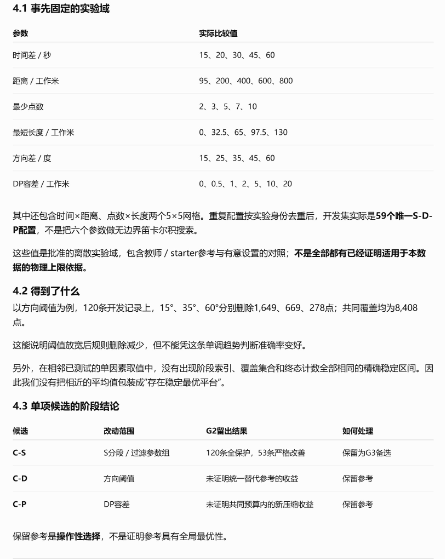
\includegraphics[width=136.500mm]{assets/crops/E12_02_02.png}};
\node[anchor=north west,inner sep=0,text width=36.40mm,align=left] at (159.60,48.51) {\color{Blue}\fontsize{9.5}{13}\selectfont \bfseries 从读数变化追问原因};
\node[anchor=north west,inner sep=0,text width=36.40mm,align=left] at (159.60,57.16) {\color{Ink}\fontsize{8.7}{12.8}\selectfont  59个去重配置覆盖三组参数实验与联合网格。后续复盘继续解释：方向阈值改变删除量，还需要检查正常信息是否被保留。};
\draw[draw=Blue,line width=.66pt,rounded corners=1mm,-{Stealth[length=1.8mm,width=1.35mm]}] (157.400,52.009) -- (153.200,52.009) -- (153.200,200.703) -- (83.937,200.703);
\draw[Rule,line width=.35pt] (14,283)--(196,283);
\node[anchor=north west,inner sep=0,text width=170.00mm,align=left] at (14.00,287.00) {\color{Muted}\fontsize{6.7}{8.5}\selectfont  智慧城市与位置服务  /  实验一过程报告  /  Part II};
\node[anchor=north west,inner sep=0,text width=11.00mm,align=left] at (185.00,286.50) {\color{Muted}\fontsize{8}{9}\selectfont  47};
\PageEnd

\PageStart
\node[anchor=north west,inner sep=0,text width=182.00mm,align=left] at (14.00,11.00) {\color{Blue}\fontsize{7.8}{10}\selectfont \bfseries PART II · 实验一中的交互与决策  /  共同评价下的实验与AI建议检验};
\node[anchor=north west,inner sep=0,text width=182.00mm,align=left] at (14.00,22.00) {\color{Ink}\fontsize{17.5}{22.5}\selectfont \bfseries 用六种真实顺序比较回答老师的问题};
\node[anchor=north west,inner sep=0,text width=182.00mm,align=left] at (14.00,33.51) {\color{Ink}\fontsize{9.5}{14.6}\selectfont  我在完整任务要求中保留了顺序讨论。执行时实际改变三步的排列，再检查断点、完整输入和最终几何关系；通过、存在权衡与被拒绝的结果都留下记录。};
\node[anchor=north west,inner sep=0] at (14,8) {\hypertarget{E13}{}};
\node[anchor=north west,inner sep=0,text width=136.50mm,align=left] at (14.00,48.63) {\color{Muted}\fontsize{7.2}{9.5}\selectfont  我要求逐项对应老师完整任务};
\node[anchor=north west,inner sep=0] at (14.000,52.828) {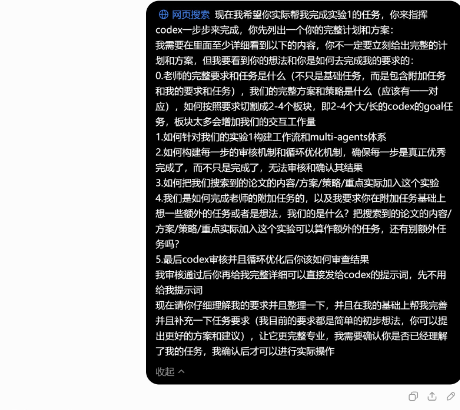
\includegraphics[width=136.500mm]{assets/crops/E13_01_01.png}};
\node[anchor=north west,inner sep=0,text width=136.50mm,align=left] at (14.00,179.69) {\color{Muted}\fontsize{7.2}{9.5}\selectfont  GPT审核六种顺序及失败原因};
\node[anchor=north west,inner sep=0] at (14.000,183.891) {
\includegraphics[width=136.500mm]{assets/crops/E13_01_02.png}};
\node[anchor=north west,inner sep=0,text width=36.40mm,align=left] at (159.60,54.63) {\color{Blue}\fontsize{9.5}{13}\selectfont \bfseries 要求实际比较};
\node[anchor=north west,inner sep=0,text width=36.40mm,align=left] at (159.60,63.28) {\color{Ink}\fontsize{8.7}{12.8}\selectfont  我要求完整覆盖老师任务并说明怎样检验。顺序实验逐一记录可用结果和失败原因，供后续解释与取舍。};
\draw[draw=Blue,line width=.66pt,rounded corners=1mm,-{Stealth[length=1.8mm,width=1.35mm]}] (157.400,58.128) -- (153.200,58.128) -- (153.200,102.384) -- (122.903,102.384);
\draw[Rule,line width=.35pt] (14,283)--(196,283);
\node[anchor=north west,inner sep=0,text width=170.00mm,align=left] at (14.00,287.00) {\color{Muted}\fontsize{6.7}{8.5}\selectfont  智慧城市与位置服务  /  实验一过程报告  /  Part II};
\node[anchor=north west,inner sep=0,text width=11.00mm,align=left] at (185.00,286.50) {\color{Muted}\fontsize{8}{9}\selectfont  48};
\PageEnd

\PageStart
\node[anchor=north west,inner sep=0,text width=182.00mm,align=left] at (14.00,11.00) {\color{Blue}\fontsize{7.8}{10}\selectfont \bfseries PART II · 实验一中的交互与决策  /  共同评价下的实验与AI建议检验};
\node[anchor=north west,inner sep=0,text width=182.00mm,align=left] at (14.00,22.00) {\color{Ink}\fontsize{17.5}{22.5}\selectfont \bfseries 用六种真实顺序比较回答老师的问题（续）};
\node[anchor=north west,inner sep=0,text width=182.00mm,align=left] at (14.00,33.51) {\color{Muted}\fontsize{8.2}{11}\selectfont  接前页，继续阅读这组对话。};
\node[anchor=north west,inner sep=0,text width=136.50mm,align=left] at (14.00,42.51) {\color{Muted}\fontsize{7.2}{9.5}\selectfont  GPT审核六种顺序及失败原因 · 续页};
\node[anchor=north west,inner sep=0] at (14.000,46.709) {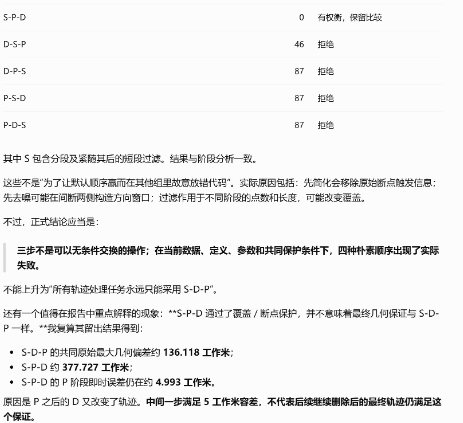
\includegraphics[width=136.500mm]{assets/crops/E13_02_01.png}};
\node[anchor=north west,inner sep=0,text width=36.40mm,align=left] at (159.60,48.51) {\color{Blue}\fontsize{9.5}{13}\selectfont \bfseries 读清各顺序的代价};
\node[anchor=north west,inner sep=0,text width=36.40mm,align=left] at (159.60,57.16) {\color{Ink}\fontsize{8.7}{12.8}\selectfont  四种顺序触发保护条件；S-P-D虽然通过部分检查，最终共同几何偏差仍高于S-D-P。GPT据此追查步骤怎样改变后续输入。};
\draw[draw=Blue,line width=.66pt,rounded corners=1mm,-{Stealth[length=1.8mm,width=1.35mm]}] (157.400,52.009) -- (153.200,52.009) -- (153.200,111.864) -- (44.071,111.864);
\draw[Rule,line width=.35pt] (14,283)--(196,283);
\node[anchor=north west,inner sep=0,text width=170.00mm,align=left] at (14.00,287.00) {\color{Muted}\fontsize{6.7}{8.5}\selectfont  智慧城市与位置服务  /  实验一过程报告  /  Part II};
\node[anchor=north west,inner sep=0,text width=11.00mm,align=left] at (185.00,286.50) {\color{Muted}\fontsize{8}{9}\selectfont  49};
\PageEnd

\PageStart
\node[anchor=north west,inner sep=0,text width=182.00mm,align=left] at (14.00,11.00) {\color{Blue}\fontsize{7.8}{10}\selectfont \bfseries PART II · 实验一中的交互与决策  /  共同评价下的实验与AI建议检验};
\node[anchor=north west,inner sep=0,text width=182.00mm,align=left] at (14.00,22.00) {\color{Ink}\fontsize{17.5}{22.5}\selectfont \bfseries 用六种真实顺序比较回答老师的问题（续）};
\node[anchor=north west,inner sep=0,text width=182.00mm,align=left] at (14.00,33.51) {\color{Muted}\fontsize{8.2}{11}\selectfont  接前页，继续阅读这组对话。};
\node[anchor=north west,inner sep=0,text width=136.50mm,align=left] at (14.00,42.51) {\color{Muted}\fontsize{7.2}{9.5}\selectfont  后续复盘：顺序为何改变结果};
\node[anchor=north west,inner sep=0] at (14.000,46.709) {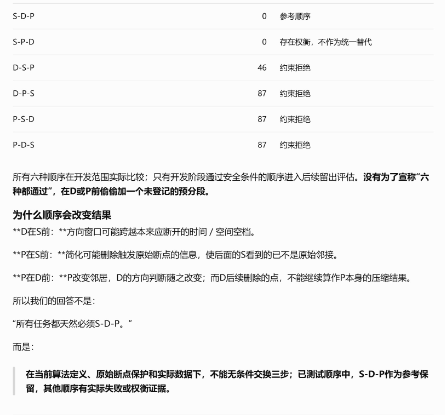
\includegraphics[width=136.500mm]{assets/crops/E13_03_01.png}};
\node[anchor=north west,inner sep=0,text width=36.40mm,align=left] at (159.60,48.51) {\color{Blue}\fontsize{9.5}{13}\selectfont \bfseries 结合本次条件解释顺序};
\node[anchor=north west,inner sep=0,text width=36.40mm,align=left] at (159.60,57.16) {\color{Ink}\fontsize{8.7}{12.8}\selectfont  在当前定义、数据和保护条件下，部分顺序被拒绝；S-P-D虽部分通过，其最终几何偏差仍与S-D-P有差异。};
\draw[draw=Blue,line width=.66pt,rounded corners=1mm,-{Stealth[length=1.8mm,width=1.35mm]}] (157.400,52.009) -- (153.200,52.009) -- (153.200,165.725) -- (67.066,165.725);
\draw[Rule,line width=.35pt] (14,283)--(196,283);
\node[anchor=north west,inner sep=0,text width=170.00mm,align=left] at (14.00,287.00) {\color{Muted}\fontsize{6.7}{8.5}\selectfont  智慧城市与位置服务  /  实验一过程报告  /  Part II};
\node[anchor=north west,inner sep=0,text width=11.00mm,align=left] at (185.00,286.50) {\color{Muted}\fontsize{8}{9}\selectfont  50};
\PageEnd

\PageStart
\node[anchor=north west,inner sep=0,text width=182.00mm,align=left] at (14.00,11.00) {\color{Blue}\fontsize{7.8}{10}\selectfont \bfseries PART II · 实验一中的交互与决策  /  共同评价下的实验与AI建议检验};
\node[anchor=north west,inner sep=0,text width=182.00mm,align=left] at (14.00,22.00) {\color{Ink}\fontsize{17.5}{22.5}\selectfont \bfseries 用真实权限和动作区分四种模式};
\node[anchor=north west,inner sep=0,text width=182.00mm,align=left] at (14.00,33.51) {\color{Ink}\fontsize{9.5}{14.6}\selectfont  我要求真实执行与共同审核。四种模式因此按实际能力区分：一次提议、确定性搜索、允许反馈，以及读取冻结记忆；每种模式的信息、动作和结果都分别检查。};
\node[anchor=north west,inner sep=0] at (14,8) {\hypertarget{E14}{}};
\node[anchor=north west,inner sep=0,text width=136.50mm,align=left] at (14.00,48.63) {\color{Muted}\fontsize{7.2}{9.5}\selectfont  前期要求：共同评价、结果为据};
\node[anchor=north west,inner sep=0] at (57.702,52.828) {
\includegraphics[width=92.798mm]{assets/crops/E14_01_01.png}};
\node[anchor=north west,inner sep=0,text width=136.50mm,align=left] at (14.00,80.69) {\color{Muted}\fontsize{7.2}{9.5}\selectfont  实施后的审核：模式实际不同};
\node[anchor=north west,inner sep=0] at (14.000,84.888) {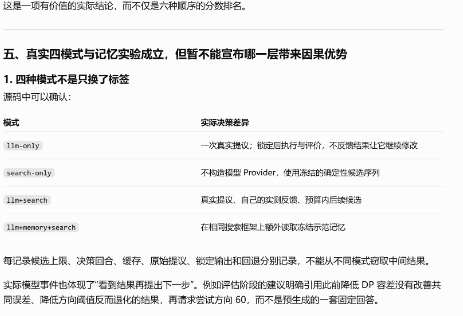
\includegraphics[width=136.500mm]{assets/crops/E14_01_02.png}};
\node[anchor=north west,inner sep=0,text width=36.40mm,align=left] at (159.60,54.63) {\color{Blue}\fontsize{9.5}{13}\selectfont \bfseries 分别检查模式的能力};
\node[anchor=north west,inner sep=0,text width=36.40mm,align=left] at (159.60,63.28) {\color{Ink}\fontsize{8.7}{12.8}\selectfont  search-only使用确定性搜索；其他模式按配置获得结果反馈或冻结记忆。实际调用记录说明各模式怎样完成任务。};
\draw[draw=Blue,line width=.66pt,rounded corners=1mm,-{Stealth[length=1.8mm,width=1.35mm]}] (157.400,58.128) -- (153.200,58.128) -- (153.200,63.484) -- (148.072,63.484);
\draw[Rule,line width=.35pt] (14,283)--(196,283);
\node[anchor=north west,inner sep=0,text width=170.00mm,align=left] at (14.00,287.00) {\color{Muted}\fontsize{6.7}{8.5}\selectfont  智慧城市与位置服务  /  实验一过程报告  /  Part II};
\node[anchor=north west,inner sep=0,text width=11.00mm,align=left] at (185.00,286.50) {\color{Muted}\fontsize{8}{9}\selectfont  51};
\PageEnd

\PageStart
\node[anchor=north west,inner sep=0,text width=182.00mm,align=left] at (14.00,11.00) {\color{Blue}\fontsize{7.8}{10}\selectfont \bfseries PART II · 实验一中的交互与决策  /  共同评价下的实验与AI建议检验};
\node[anchor=north west,inner sep=0,text width=182.00mm,align=left] at (14.00,22.00) {\color{Ink}\fontsize{17.5}{22.5}\selectfont \bfseries 用真实权限和动作区分四种模式（续）};
\node[anchor=north west,inner sep=0,text width=182.00mm,align=left] at (14.00,33.51) {\color{Muted}\fontsize{8.2}{11}\selectfont  接前页，继续阅读这组对话。};
\node[anchor=north west,inner sep=0,text width=136.50mm,align=left] at (14.00,42.51) {\color{Muted}\fontsize{7.2}{9.5}\selectfont  后续复盘：权限与84次有效实验};
\node[anchor=north west,inner sep=0] at (14.000,46.709) {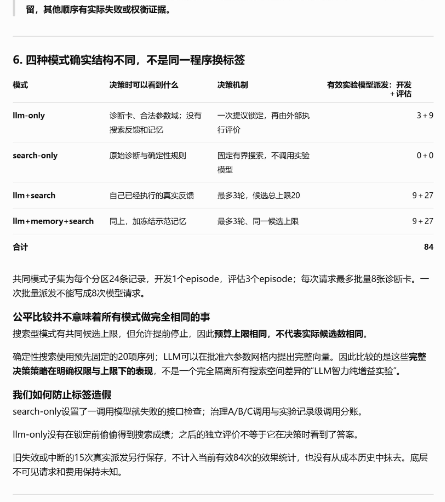
\includegraphics[width=136.500mm]{assets/crops/E14_02_01.png}};
\node[anchor=north west,inner sep=0,text width=36.40mm,align=left] at (159.60,48.51) {\color{Blue}\fontsize{9.5}{13}\selectfont \bfseries 把调用口径说明白};
\node[anchor=north west,inner sep=0,text width=36.40mm,align=left] at (159.60,57.16) {\color{Ink}\fontsize{8.7}{12.8}\selectfont  84次统计的是记录级有效实验，开发与评价分别记录。各模式的共同预算上限相同，实际动作和消耗则按运行结果说明。};
\draw[draw=Blue,line width=.66pt,rounded corners=1mm,-{Stealth[length=1.8mm,width=1.35mm]}] (157.400,52.009) -- (153.200,52.009) -- (153.200,148.854) -- (127.494,148.854);
\draw[Rule,line width=.35pt] (14,283)--(196,283);
\node[anchor=north west,inner sep=0,text width=170.00mm,align=left] at (14.00,287.00) {\color{Muted}\fontsize{6.7}{8.5}\selectfont  智慧城市与位置服务  /  实验一过程报告  /  Part II};
\node[anchor=north west,inner sep=0,text width=11.00mm,align=left] at (185.00,286.50) {\color{Muted}\fontsize{8}{9}\selectfont  52};
\PageEnd

\PageStart
\node[anchor=north west,inner sep=0,text width=182.00mm,align=left] at (14.00,11.00) {\color{Blue}\fontsize{7.8}{10}\selectfont \bfseries PART II · 实验一中的交互与决策  /  共同评价下的实验与AI建议检验};
\node[anchor=north west,inner sep=0,text width=182.00mm,align=left] at (14.00,22.00) {\color{Ink}\fontsize{17.5}{22.5}\selectfont \bfseries 沿着送达、引用和动作检查记忆的作用};
\node[anchor=north west,inner sep=0,text width=182.00mm,align=left] at (14.00,33.51) {\color{Ink}\fontsize{9.5}{14.6}\selectfont  我提出的“结果必须有依据”同样适用于记忆。后续核验逐层检查经验来自哪里、是否送达、是否被引用，以及实际动作是否与引用一致，再判断这些证据能支持怎样的结论。};
\node[anchor=north west,inner sep=0] at (14,8) {\hypertarget{E15}{}};
\node[anchor=north west,inner sep=0,text width=136.50mm,align=left] at (14.00,48.63) {\color{Muted}\fontsize{7.2}{9.5}\selectfont  回引前期要求：所有结果都要有依据};
\node[anchor=north west,inner sep=0] at (57.702,52.828) {
\includegraphics[width=92.798mm]{assets/crops/E15_01_01.png}};
\node[anchor=north west,inner sep=0,text width=136.50mm,align=left] at (14.00,80.69) {\color{Muted}\fontsize{7.2}{9.5}\selectfont  后续复盘：送达、引用与动作};
\node[anchor=north west,inner sep=0] at (14.000,84.888) {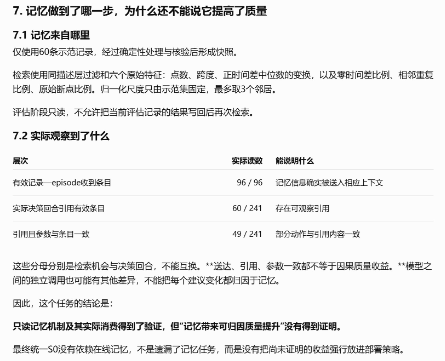
\includegraphics[width=136.500mm]{assets/crops/E15_01_02.png}};
\node[anchor=north west,inner sep=0,text width=136.50mm,align=left] at (14.00,200.82) {\color{Muted}\fontsize{7.2}{9.5}\selectfont  阶段审核保留的结论边界};
\node[anchor=north west,inner sep=0] at (14.000,205.022) {
\includegraphics[width=136.500mm]{assets/crops/E15_01_03.png}};
\node[anchor=north west,inner sep=0,text width=36.40mm,align=left] at (159.60,54.63) {\color{Blue}\fontsize{9.5}{13}\selectfont \bfseries 分层检查实际使用};
\node[anchor=north west,inner sep=0,text width=36.40mm,align=left] at (159.60,63.28) {\color{Ink}\fontsize{8.7}{12.8}\selectfont  记忆的送达、引用与动作一致分别记录。这样能够看清经验在哪一步被使用，也能定位检索与实际决策之间的差别。};
\draw[draw=Blue,line width=.66pt,rounded corners=1mm,-{Stealth[length=1.8mm,width=1.35mm]}] (157.400,58.128) -- (153.200,58.128) -- (153.200,63.484) -- (148.072,63.484);
\node[anchor=north west,inner sep=0,text width=36.40mm,align=left] at (159.60,104.89) {\color{Violet}\fontsize{9.5}{13}\selectfont \bfseries 按证据决定是否保留};
\node[anchor=north west,inner sep=0,text width=36.40mm,align=left] at (159.60,113.54) {\color{Ink}\fontsize{8.7}{12.8}\selectfont  运行记录显示记忆已被使用，但本轮证据尚不足以确认它带来的质量收益。因此最终固定处理采用无记忆设置。};
\draw[draw=Violet,line width=.66pt,rounded corners=1mm,-{Stealth[length=1.8mm,width=1.35mm]}] (157.400,108.388) -- (155.300,108.388) -- (155.300,230.671) -- (138.118,230.671);
\draw[Rule,line width=.35pt] (14,283)--(196,283);
\node[anchor=north west,inner sep=0,text width=170.00mm,align=left] at (14.00,287.00) {\color{Muted}\fontsize{6.7}{8.5}\selectfont  智慧城市与位置服务  /  实验一过程报告  /  Part II};
\node[anchor=north west,inner sep=0,text width=11.00mm,align=left] at (185.00,286.50) {\color{Muted}\fontsize{8}{9}\selectfont  53};
\PageEnd

\PageStart
\node[anchor=north west,inner sep=0,text width=182.00mm,align=left] at (14.00,11.00) {\color{Blue}\fontsize{7.8}{10}\selectfont \bfseries PART II · 实验一中的交互与决策  /  共同评价下的实验与AI建议检验};
\node[anchor=north west,inner sep=0,text width=182.00mm,align=left] at (14.00,22.00) {\color{Ink}\fontsize{17.5}{22.5}\selectfont \bfseries 用共同参考检验一条AI建议};
\node[anchor=north west,inner sep=0,text width=182.00mm,align=left] at (14.00,33.51) {\color{Ink}\fontsize{9.5}{14.6}\selectfont  记录7764提供了一个具体案例：模型建议可以执行，候选自身的DP检查也通过，但回到共同原始参考时，几何偏差增大了。我前面提出的真实执行与共同评价要求，在这里进入了实际判断。};
\node[anchor=north west,inner sep=0] at (14,8) {\hypertarget{E16}{}};
\node[anchor=north west,inner sep=0,text width=136.50mm,align=left] at (14.00,48.63) {\color{Muted}\fontsize{7.2}{9.5}\selectfont  我的前期规则授权};
\node[anchor=north west,inner sep=0] at (57.702,52.828) {
\includegraphics[width=92.798mm]{assets/crops/E16_01_01.png}};
\node[anchor=north west,inner sep=0,text width=136.50mm,align=left] at (14.00,80.69) {\color{Muted}\fontsize{7.2}{9.5}\selectfont  阶段审核中的真实建议核验};
\node[anchor=north west,inner sep=0] at (14.000,84.888) {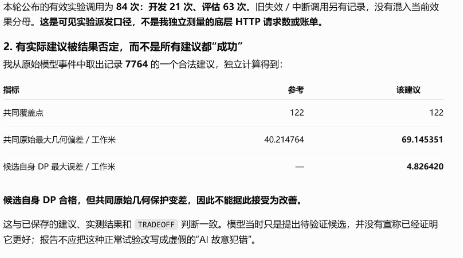
\includegraphics[width=136.500mm]{assets/crops/E16_01_02.png}};
\node[anchor=north west,inner sep=0,text width=136.50mm,align=left] at (14.00,166.15) {\color{Muted}\fontsize{7.2}{9.5}\selectfont  后续复盘：局部与整链保证};
\node[anchor=north west,inner sep=0] at (14.000,170.351) {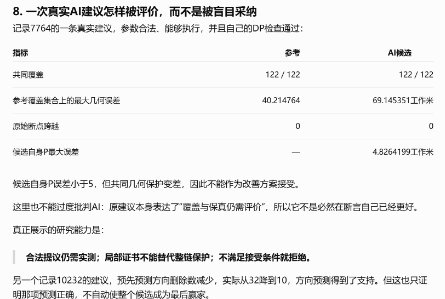
\includegraphics[width=136.500mm]{assets/crops/E16_01_03.png}};
\node[anchor=north west,inner sep=0,text width=36.40mm,align=left] at (159.60,54.63) {\color{Blue}\fontsize{9.5}{13}\selectfont \bfseries 前期要求在案例中落实};
\node[anchor=north west,inner sep=0,text width=36.40mm,align=left] at (159.60,63.28) {\color{Ink}\fontsize{8.7}{12.8}\selectfont  我先要求结果经过共同评价；记录7764的问题随后在执行与核验中显现，成为检查建议采用依据的具体案例。};
\draw[draw=Blue,line width=.66pt,rounded corners=1mm,-{Stealth[length=1.8mm,width=1.35mm]}] (157.400,58.128) -- (153.200,58.128) -- (153.200,63.484) -- (148.072,63.484);
\node[anchor=north west,inner sep=0,text width=36.40mm,align=left] at (159.60,104.89) {\color{Violet}\fontsize{9.5}{13}\selectfont \bfseries 共同参考给出采用依据};
\node[anchor=north west,inner sep=0,text width=36.40mm,align=left] at (159.60,113.54) {\color{Ink}\fontsize{8.7}{12.8}\selectfont  共同几何偏差约由40.215增至69.145工作米。候选自身DP约4.826工作米，最终因共同几何保护未满足而未被采用。};
\draw[draw=Violet,line width=.66pt,rounded corners=1mm,-{Stealth[length=1.8mm,width=1.35mm]}] (157.400,108.388) -- (155.300,108.388) -- (155.300,249.184) -- (110.010,249.184);
\node[anchor=north west,inner sep=0,text width=36.40mm,align=left] at (159.60,155.15) {\color{Rose}\fontsize{8.9}{12.5}\selectfont \bfseries 我的回看};
\node[anchor=north west,inner sep=0,text width=36.40mm,align=left] at (159.60,162.15) {\color{Ink}\fontsize{8.5}{12.7}\selectfont  回看这条建议，我更能理解局部算法检查与完整处理效果的差别：采用决定还要检查前后处理对同一原始参考的影响。};
\draw[Rule,line width=.35pt] (14,283)--(196,283);
\node[anchor=north west,inner sep=0,text width=170.00mm,align=left] at (14.00,287.00) {\color{Muted}\fontsize{6.7}{8.5}\selectfont  智慧城市与位置服务  /  实验一过程报告  /  Part II};
\node[anchor=north west,inner sep=0,text width=11.00mm,align=left] at (185.00,286.50) {\color{Muted}\fontsize{8}{9}\selectfont  54};
\PageEnd

\PageStart
\node[anchor=north west,inner sep=0,text width=182.00mm,align=left] at (14.00,11.00) {\color{Blue}\fontsize{7.8}{10}\selectfont \bfseries PART II · 实验一中的交互与决策  /  方案组合、回退与最终确认};
\node[anchor=north west,inner sep=0,text width=182.00mm,align=left] at (14.00,22.00) {\color{Ink}\fontsize{17.5}{22.5}\selectfont \bfseries 先确定选择规则，再由结果决定方案};
\node[anchor=north west,inner sep=0,text width=182.00mm,align=left] at (14.00,33.51) {\color{Ink}\fontsize{9.5}{14.6}\selectfont  进入Goal 3时，我问能否让Codex依据实验完成候选、比较和选择。随后我与GPT明确了范围、预算和判定条件，把具体方案的取舍交给这些规则下的真实结果。};
\node[anchor=north west,inner sep=0] at (14,8) {\hypertarget{E17}{}};
\node[anchor=north west,inner sep=0,text width=136.50mm,align=left] at (14.00,48.63) {\color{Muted}\fontsize{7.2}{9.5}\selectfont  我提出结果驱动的下一阶段};
\node[anchor=north west,inner sep=0] at (14.000,52.828) {
\includegraphics[width=136.500mm]{assets/crops/E17_01_01.png}};
\node[anchor=north west,inner sep=0,text width=136.50mm,align=left] at (14.00,101.82) {\color{Muted}\fontsize{7.2}{9.5}\selectfont  GPT修订范围、规则和交付};
\node[anchor=north west,inner sep=0] at (14.000,106.018) {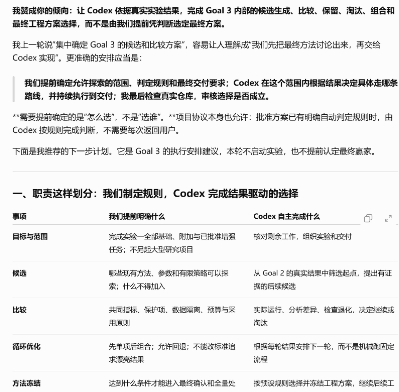
\includegraphics[width=136.500mm]{assets/crops/E17_01_02.png}};
\node[anchor=north west,inner sep=0,text width=36.40mm,align=left] at (159.60,54.63) {\color{Blue}\fontsize{9.5}{13}\selectfont \bfseries 先把选择条件讲清};
\node[anchor=north west,inner sep=0,text width=36.40mm,align=left] at (159.60,63.28) {\color{Ink}\fontsize{8.7}{12.8}\selectfont  候选需要明确的范围、预算、保护条件和可复查结果。重要方法或评价变化，则重新回到讨论中判断。};
\draw[draw=Blue,line width=.66pt,rounded corners=1mm,-{Stealth[length=1.8mm,width=1.35mm]}] (157.400,58.128) -- (153.200,58.128) -- (153.200,85.499) -- (75.579,85.499);
\draw[Rule,line width=.35pt] (14,283)--(196,283);
\node[anchor=north west,inner sep=0,text width=170.00mm,align=left] at (14.00,287.00) {\color{Muted}\fontsize{6.7}{8.5}\selectfont  智慧城市与位置服务  /  实验一过程报告  /  Part II};
\node[anchor=north west,inner sep=0,text width=11.00mm,align=left] at (185.00,286.50) {\color{Muted}\fontsize{8}{9}\selectfont  55};
\PageEnd

\PageStart
\node[anchor=north west,inner sep=0,text width=182.00mm,align=left] at (14.00,11.00) {\color{Blue}\fontsize{7.8}{10}\selectfont \bfseries PART II · 实验一中的交互与决策  /  方案组合、回退与最终确认};
\node[anchor=north west,inner sep=0,text width=182.00mm,align=left] at (14.00,22.00) {\color{Ink}\fontsize{17.5}{22.5}\selectfont \bfseries 先确定选择规则，再由结果决定方案（续）};
\node[anchor=north west,inner sep=0,text width=182.00mm,align=left] at (14.00,33.51) {\color{Muted}\fontsize{8.2}{11}\selectfont  接前页，继续阅读这组对话。};
\node[anchor=north west,inner sep=0,text width=136.50mm,align=left] at (14.00,42.51) {\color{Muted}\fontsize{7.2}{9.5}\selectfont  GPT修订范围、规则和交付 · 续页};
\node[anchor=north west,inner sep=0] at (14.000,46.709) {
\includegraphics[width=136.500mm]{assets/crops/E17_02_01.png}};
\node[anchor=north west,inner sep=0,text width=136.50mm,align=left] at (14.00,83.38) {\color{Muted}\fontsize{7.2}{9.5}\selectfont  同一回答：选择、冻结和确认分开};
\node[anchor=north west,inner sep=0] at (14.000,87.583) {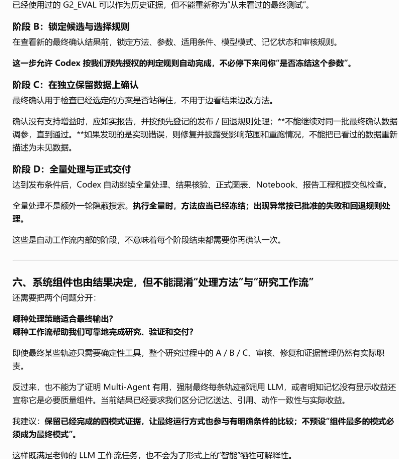
\includegraphics[width=136.500mm]{assets/crops/E17_02_02.png}};
\node[anchor=north west,inner sep=0,text width=36.40mm,align=left] at (159.60,48.51) {\color{Blue}\fontsize{9.5}{13}\selectfont \bfseries 为最终确认保留数据};
\node[anchor=north west,inner sep=0,text width=36.40mm,align=left] at (159.60,57.16) {\color{Ink}\fontsize{8.7}{12.8}\selectfont  已看过的评价数据继续作为开发证据。方法固定后，再使用预先保留的记录检查选定方案。};
\draw[draw=Blue,line width=.66pt,rounded corners=1mm,-{Stealth[length=1.8mm,width=1.35mm]}] (157.400,52.009) -- (153.200,52.009) -- (153.200,196.544) -- (54.026,196.544);
\draw[Rule,line width=.35pt] (14,283)--(196,283);
\node[anchor=north west,inner sep=0,text width=170.00mm,align=left] at (14.00,287.00) {\color{Muted}\fontsize{6.7}{8.5}\selectfont  智慧城市与位置服务  /  实验一过程报告  /  Part II};
\node[anchor=north west,inner sep=0,text width=11.00mm,align=left] at (185.00,286.50) {\color{Muted}\fontsize{8}{9}\selectfont  56};
\PageEnd

\PageStart
\node[anchor=north west,inner sep=0,text width=182.00mm,align=left] at (14.00,11.00) {\color{Blue}\fontsize{7.8}{10}\selectfont \bfseries PART II · 实验一中的交互与决策  /  方案组合、回退与最终确认};
\node[anchor=north west,inner sep=0,text width=182.00mm,align=left] at (14.00,22.00) {\color{Ink}\fontsize{17.5}{22.5}\selectfont \bfseries 组合经历支持与退化，最后回到简单方案};
\node[anchor=north west,inner sep=0,text width=182.00mm,align=left] at (14.00,33.51) {\color{Ink}\fontsize{9.5}{14.6}\selectfont  我要求先单项、再组合，好的保留、退化回退。实际比较中，组合曾获得开发数据支持，但在新的选择记录上出现三条几何退化，于是按原定规则退出。};
\node[anchor=north west,inner sep=0] at (14,8) {\hypertarget{E18}{}};
\node[anchor=north west,inner sep=0,text width=136.50mm,align=left] at (14.00,48.63) {\color{Muted}\fontsize{7.2}{9.5}\selectfont  我的原始要求：先验证，再组合};
\node[anchor=north west,inner sep=0] at (57.702,52.828) {
\includegraphics[width=92.798mm]{assets/crops/E18_01_01.png}};
\node[anchor=north west,inner sep=0,text width=136.50mm,align=left] at (14.00,76.64) {\color{Muted}\fontsize{7.2}{9.5}\selectfont  Goal 3真实结果：退化与回退};
\node[anchor=north west,inner sep=0] at (14.000,80.842) {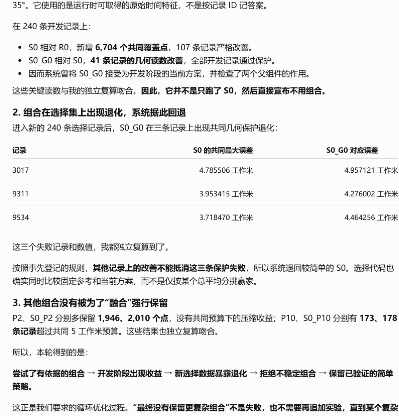
\includegraphics[width=136.500mm]{assets/crops/E18_01_02.png}};
\node[anchor=north west,inner sep=0,text width=36.40mm,align=left] at (159.60,54.63) {\color{Blue}\fontsize{9.5}{13}\selectfont \bfseries 新记录改变了选择};
\node[anchor=north west,inner sep=0,text width=36.40mm,align=left] at (159.60,63.28) {\color{Ink}\fontsize{8.7}{12.8}\selectfont  S0与方向条件规则的组合在3017、9311、9534上退化。三条失败触发共同保护规则，组合因此被撤回。};
\draw[draw=Blue,line width=.66pt,rounded corners=1mm,-{Stealth[length=1.8mm,width=1.35mm]}] (157.400,58.128) -- (153.200,58.128) -- (153.200,59.707) -- (148.072,59.707);
\draw[Rule,line width=.35pt] (14,283)--(196,283);
\node[anchor=north west,inner sep=0,text width=170.00mm,align=left] at (14.00,287.00) {\color{Muted}\fontsize{6.7}{8.5}\selectfont  智慧城市与位置服务  /  实验一过程报告  /  Part II};
\node[anchor=north west,inner sep=0,text width=11.00mm,align=left] at (185.00,286.50) {\color{Muted}\fontsize{8}{9}\selectfont  57};
\PageEnd

\PageStart
\node[anchor=north west,inner sep=0,text width=182.00mm,align=left] at (14.00,11.00) {\color{Blue}\fontsize{7.8}{10}\selectfont \bfseries PART II · 实验一中的交互与决策  /  方案组合、回退与最终确认};
\node[anchor=north west,inner sep=0,text width=182.00mm,align=left] at (14.00,22.00) {\color{Ink}\fontsize{17.5}{22.5}\selectfont \bfseries 组合经历支持与退化，最后回到简单方案（续）};
\node[anchor=north west,inner sep=0,text width=182.00mm,align=left] at (14.00,33.51) {\color{Muted}\fontsize{8.2}{11}\selectfont  接前页，继续阅读这组对话。};
\node[anchor=north west,inner sep=0,text width=136.50mm,align=left] at (14.00,42.51) {\color{Muted}\fontsize{7.2}{9.5}\selectfont  后续复盘：单项、父项与组合};
\node[anchor=north west,inner sep=0] at (14.000,46.709) {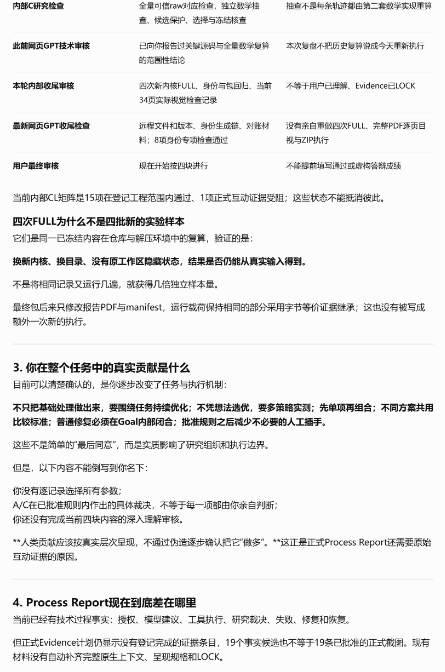
\includegraphics[width=136.500mm]{assets/crops/E18_02_01.png}};
\node[anchor=north west,inner sep=0,text width=36.40mm,align=left] at (159.60,48.51) {\color{Blue}\fontsize{9.5}{13}\selectfont \bfseries 回看我的研究要求};
\node[anchor=north west,inner sep=0,text width=36.40mm,align=left] at (159.60,57.16) {\color{Ink}\fontsize{8.7}{12.8}\selectfont  后续复盘把我的作用归到任务与判断规则：先单项再组合、共同评价、退化回退。具体候选由真实比较逐步筛选。};
\draw[draw=Blue,line width=.66pt,rounded corners=1mm,-{Stealth[length=1.8mm,width=1.35mm]}] (157.400,52.009) -- (153.200,52.009) -- (153.200,236.582) -- (121.973,236.582);
\node[anchor=north west,inner sep=0,text width=36.40mm,align=left] at (159.60,98.77) {\color{Rose}\fontsize{8.9}{12.5}\selectfont \bfseries 我的回看};
\node[anchor=north west,inner sep=0,text width=36.40mm,align=left] at (159.60,105.77) {\color{Ink}\fontsize{8.5}{12.7}\selectfont  S0包含点数和长度两项过滤调整。后续分别检查它们的作用，再判断两项调整合用时留下了什么。};
\draw[Rule,line width=.35pt] (14,283)--(196,283);
\node[anchor=north west,inner sep=0,text width=170.00mm,align=left] at (14.00,287.00) {\color{Muted}\fontsize{6.7}{8.5}\selectfont  智慧城市与位置服务  /  实验一过程报告  /  Part II};
\node[anchor=north west,inner sep=0,text width=11.00mm,align=left] at (185.00,286.50) {\color{Muted}\fontsize{8}{9}\selectfont  58};
\PageEnd

\PageStart
\node[anchor=north west,inner sep=0,text width=182.00mm,align=left] at (14.00,11.00) {\color{Blue}\fontsize{7.8}{10}\selectfont \bfseries PART II · 实验一中的交互与决策  /  方案组合、回退与最终确认  /  关系图};
\node[anchor=north west,inner sep=0,text width=182.00mm,align=left] at (14.00,25.00) {\color{Ink}\fontsize{18}{24}\selectfont \bfseries 单项、组合、选择与回退的真实路径};
\node[anchor=north west,inner sep=0,text width=182.00mm,align=left] at (14.00,43.00) {\color{Ink}\fontsize{9.6}{15}\selectfont  先看各项调整的独立作用，再用新的选择记录检查组合；三条几何退化使方案回到S0。};
\node[anchor=north west,inner sep=0] at (14,71) {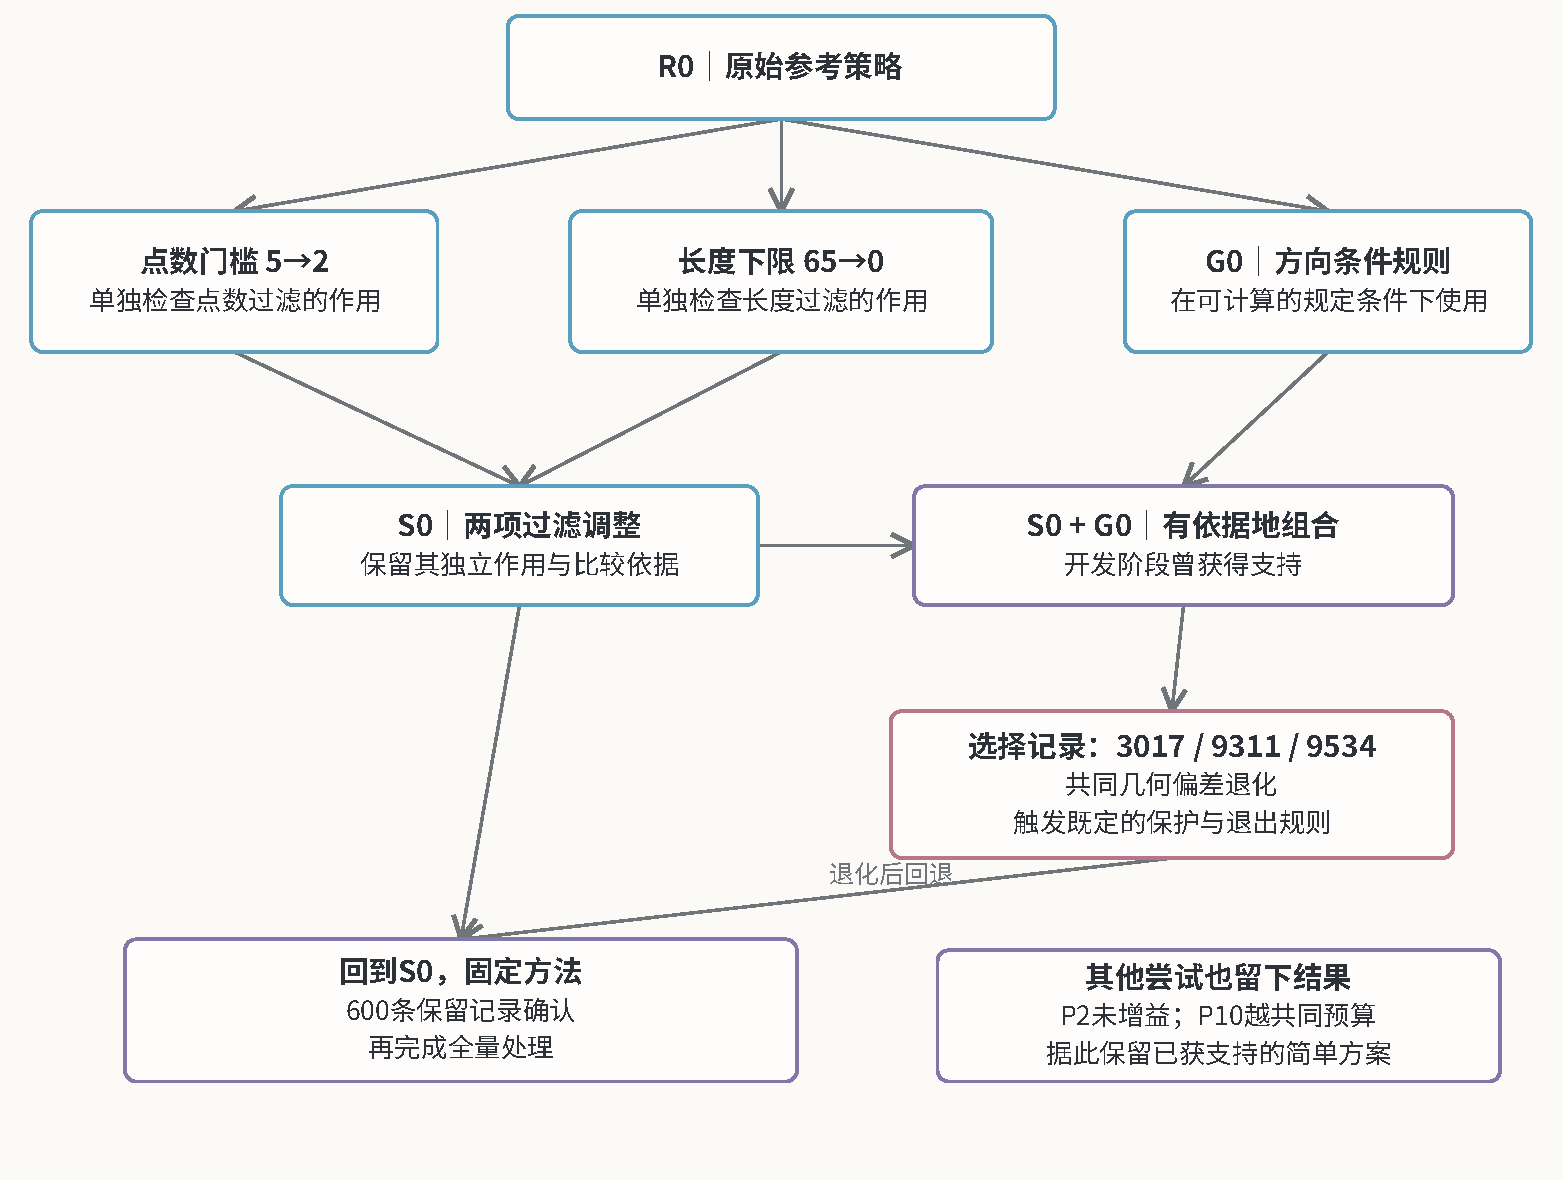
\includegraphics[width=182mm]{figures/D04.pdf}};
\node[anchor=north west,inner sep=0,text width=182.00mm,align=left] at (14.00,218.41) {\color{Ink}\fontsize{10}{15.5}\selectfont  开发阶段曾支持S0与G0组合，新的选择记录随后触发保护条件。最终保留S0，固定方法后完成600条确认记录与全量处理。};
\draw[Rule,line width=.35pt] (14,283)--(196,283);
\node[anchor=north west,inner sep=0,text width=170.00mm,align=left] at (14.00,287.00) {\color{Muted}\fontsize{6.7}{8.5}\selectfont  智慧城市与位置服务  /  实验一过程报告  /  Part II};
\node[anchor=north west,inner sep=0,text width=11.00mm,align=left] at (185.00,286.50) {\color{Muted}\fontsize{8}{9}\selectfont  59};
\PageEnd

\PageStart
\node[anchor=north west,inner sep=0,text width=182.00mm,align=left] at (14.00,11.00) {\color{Blue}\fontsize{7.8}{10}\selectfont \bfseries PART II · 实验一中的交互与决策  /  方案组合、回退与最终确认};
\node[anchor=north west,inner sep=0,text width=182.00mm,align=left] at (14.00,22.00) {\color{Ink}\fontsize{17.5}{22.5}\selectfont \bfseries 从冻结确认到全量处理，读清最终结果};
\node[anchor=north west,inner sep=0,text width=182.00mm,align=left] at (14.00,33.51) {\color{Ink}\fontsize{9.5}{14.6}\selectfont  Codex完成Goal 3后，我把交付返回GPT核查。GPT先确认选定方案与冻结时点，再核对600条保留记录和全量处理，并结合收益来源与边界案例解释这些数字。};
\node[anchor=north west,inner sep=0] at (14,8) {\hypertarget{E19}{}};
\node[anchor=north west,inner sep=0,text width=136.50mm,align=left] at (14.00,48.63) {\color{Muted}\fontsize{7.2}{9.5}\selectfont  我转交的Goal 3回复与审核开头};
\node[anchor=north west,inner sep=0] at (14.000,52.828) {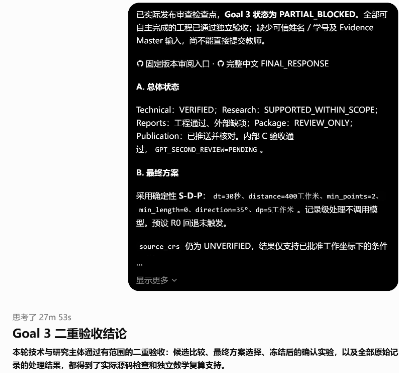
\includegraphics[width=136.500mm]{assets/crops/E19_01_01.png}};
\node[anchor=north west,inner sep=0,text width=136.50mm,align=left] at (14.00,185.63) {\color{Muted}\fontsize{7.2}{9.5}\selectfont  冻结后的600条确认记录};
\node[anchor=north west,inner sep=0] at (14.000,189.833) {
\includegraphics[width=136.500mm]{assets/crops/E19_01_02.png}};
\node[anchor=north west,inner sep=0,text width=36.40mm,align=left] at (159.60,54.63) {\color{Blue}\fontsize{9.5}{13}\selectfont \bfseries 分别核对确认与生产};
\node[anchor=north west,inner sep=0,text width=36.40mm,align=left] at (159.60,63.28) {\color{Ink}\fontsize{8.7}{12.8}\selectfont  我转交Codex的交付回执，GPT继续检查冻结时点、600条确认和全量结果，分别说明它们的用途。};
\draw[draw=Blue,line width=.66pt,rounded corners=1mm,-{Stealth[length=1.8mm,width=1.35mm]}] (157.400,58.128) -- (153.200,58.128) -- (153.200,82.420) -- (76.605,82.420);
\draw[Rule,line width=.35pt] (14,283)--(196,283);
\node[anchor=north west,inner sep=0,text width=170.00mm,align=left] at (14.00,287.00) {\color{Muted}\fontsize{6.7}{8.5}\selectfont  智慧城市与位置服务  /  实验一过程报告  /  Part II};
\node[anchor=north west,inner sep=0,text width=11.00mm,align=left] at (185.00,286.50) {\color{Muted}\fontsize{8}{9}\selectfont  60};
\PageEnd

\PageStart
\node[anchor=north west,inner sep=0,text width=182.00mm,align=left] at (14.00,11.00) {\color{Blue}\fontsize{7.8}{10}\selectfont \bfseries PART II · 实验一中的交互与决策  /  方案组合、回退与最终确认};
\node[anchor=north west,inner sep=0,text width=182.00mm,align=left] at (14.00,22.00) {\color{Ink}\fontsize{17.5}{22.5}\selectfont \bfseries 从冻结确认到全量处理，读清最终结果（续）};
\node[anchor=north west,inner sep=0,text width=182.00mm,align=left] at (14.00,33.51) {\color{Muted}\fontsize{8.2}{11}\selectfont  接前页，继续阅读这组对话。};
\node[anchor=north west,inner sep=0,text width=136.50mm,align=left] at (14.00,42.51) {\color{Muted}\fontsize{7.2}{9.5}\selectfont  冻结后的600条确认记录 · 续页};
\node[anchor=north west,inner sep=0] at (14.000,46.709) {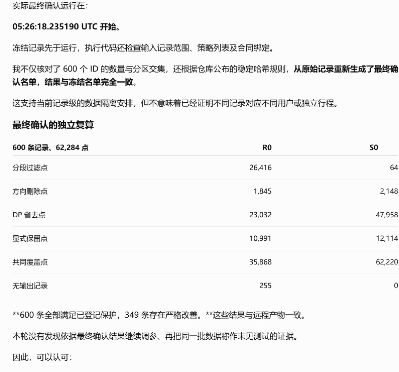
\includegraphics[width=136.500mm]{assets/crops/E19_02_01.png}};
\node[anchor=north west,inner sep=0,text width=136.50mm,align=left] at (14.00,179.17) {\color{Muted}\fontsize{7.2}{9.5}\selectfont  全量复算与收益来源};
\node[anchor=north west,inner sep=0] at (14.000,183.373) {
\includegraphics[width=136.500mm]{assets/crops/E19_02_02.png}};
\node[anchor=north west,inner sep=0,text width=36.40mm,align=left] at (159.60,48.51) {\color{Blue}\fontsize{9.5}{13}\selectfont \bfseries 冻结之后再确认};
\node[anchor=north west,inner sep=0,text width=36.40mm,align=left] at (159.60,57.16) {\color{Ink}\fontsize{8.7}{12.8}\selectfont  GPT核对冻结时点与600条确认记录：方案固定在先，运行在后。全部记录满足既定保护，其中349条记录有严格改善。};
\draw[draw=Blue,line width=.66pt,rounded corners=1mm,-{Stealth[length=1.8mm,width=1.35mm]}] (157.400,52.009) -- (153.200,52.009) -- (153.200,161.486) -- (116.632,161.486);
\draw[Rule,line width=.35pt] (14,283)--(196,283);
\node[anchor=north west,inner sep=0,text width=170.00mm,align=left] at (14.00,287.00) {\color{Muted}\fontsize{6.7}{8.5}\selectfont  智慧城市与位置服务  /  实验一过程报告  /  Part II};
\node[anchor=north west,inner sep=0,text width=11.00mm,align=left] at (185.00,286.50) {\color{Muted}\fontsize{8}{9}\selectfont  61};
\PageEnd

\PageStart
\node[anchor=north west,inner sep=0,text width=182.00mm,align=left] at (14.00,11.00) {\color{Blue}\fontsize{7.8}{10}\selectfont \bfseries PART II · 实验一中的交互与决策  /  方案组合、回退与最终确认};
\node[anchor=north west,inner sep=0,text width=182.00mm,align=left] at (14.00,22.00) {\color{Ink}\fontsize{17.5}{22.5}\selectfont \bfseries 从冻结确认到全量处理，读清最终结果（续）};
\node[anchor=north west,inner sep=0,text width=182.00mm,align=left] at (14.00,33.51) {\color{Muted}\fontsize{8.2}{11}\selectfont  接前页，继续阅读这组对话。};
\node[anchor=north west,inner sep=0,text width=136.50mm,align=left] at (14.00,42.51) {\color{Muted}\fontsize{7.2}{9.5}\selectfont  全量复算与收益来源 · 续页};
\node[anchor=north west,inner sep=0] at (14.000,46.709) {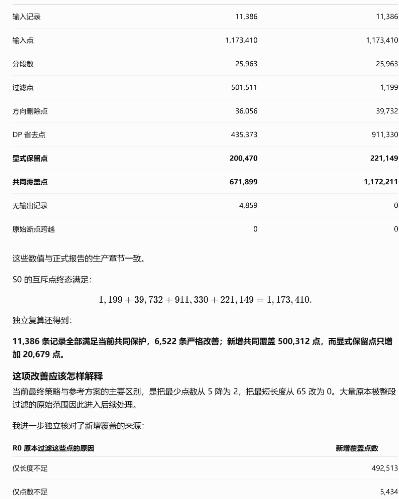
\includegraphics[width=136.500mm]{assets/crops/E19_03_01.png}};
\node[anchor=north west,inner sep=0,text width=36.40mm,align=left] at (159.60,48.51) {\color{Blue}\fontsize{9.5}{13}\selectfont \bfseries 覆盖增加来自哪里};
\node[anchor=north west,inner sep=0,text width=36.40mm,align=left] at (159.60,57.16) {\color{Ink}\fontsize{8.7}{12.8}\selectfont  全量核对显示，共同覆盖增加500,312点，显式保留增加20,679点。GPT继续按原过滤原因分解收益，把主要变化追溯到短片段过滤条件。};
\draw[Rule,line width=.35pt] (14,283)--(196,283);
\node[anchor=north west,inner sep=0,text width=170.00mm,align=left] at (14.00,287.00) {\color{Muted}\fontsize{6.7}{8.5}\selectfont  智慧城市与位置服务  /  实验一过程报告  /  Part II};
\node[anchor=north west,inner sep=0,text width=11.00mm,align=left] at (185.00,286.50) {\color{Muted}\fontsize{8}{9}\selectfont  62};
\PageEnd

\PageStart
\node[anchor=north west,inner sep=0,text width=182.00mm,align=left] at (14.00,11.00) {\color{Blue}\fontsize{7.8}{10}\selectfont \bfseries PART II · 实验一中的交互与决策  /  方案组合、回退与最终确认};
\node[anchor=north west,inner sep=0,text width=182.00mm,align=left] at (14.00,22.00) {\color{Ink}\fontsize{17.5}{22.5}\selectfont \bfseries 从冻结确认到全量处理，读清最终结果（续）};
\node[anchor=north west,inner sep=0,text width=182.00mm,align=left] at (14.00,33.51) {\color{Muted}\fontsize{8.2}{11}\selectfont  接前页，继续阅读这组对话。};
\node[anchor=north west,inner sep=0,text width=136.50mm,align=left] at (14.00,42.51) {\color{Muted}\fontsize{7.2}{9.5}\selectfont  全量复算与收益来源 · 续页};
\node[anchor=north west,inner sep=0] at (14.000,46.709) {
\includegraphics[width=136.500mm]{assets/crops/E19_04_01.png}};
\node[anchor=north west,inner sep=0,text width=136.50mm,align=left] at (14.00,83.73) {\color{Muted}\fontsize{7.2}{9.5}\selectfont  同一轮：约266工作米的边界案例};
\node[anchor=north west,inner sep=0] at (14.000,87.925) {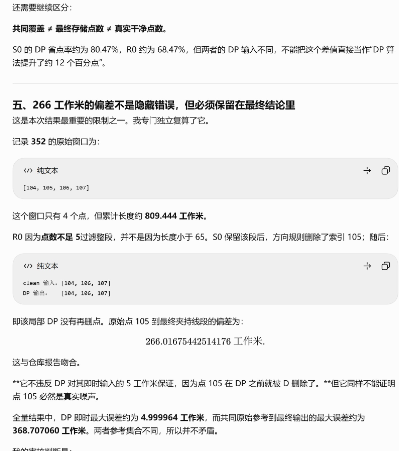
\includegraphics[width=136.500mm]{assets/crops/E19_04_02.png}};
\node[anchor=north west,inner sep=0,text width=36.40mm,align=left] at (159.60,48.51) {\color{Blue}\fontsize{9.5}{13}\selectfont \bfseries 把边界案例留在结论中};
\node[anchor=north west,inner sep=0,text width=36.40mm,align=left] at (159.60,57.16) {\color{Ink}\fontsize{8.7}{12.8}\selectfont  新增覆盖主要来自减少短段过滤损失。记录352的点105在DP之前被删除，它不在DP的5工作米保证范围内。};
\draw[draw=Blue,line width=.66pt,rounded corners=1mm,-{Stealth[length=1.8mm,width=1.35mm]}] (157.400,52.009) -- (153.200,52.009) -- (153.200,204.412) -- (105.684,204.412);
\node[anchor=north west,inner sep=0,text width=36.40mm,align=left] at (159.60,94.25) {\color{Rose}\fontsize{8.9}{12.5}\selectfont \bfseries 我的回看};
\node[anchor=north west,inner sep=0,text width=36.40mm,align=left] at (159.60,101.25) {\color{Ink}\fontsize{8.5}{12.7}\selectfont  本轮改善得到共同覆盖与几何保护的支持；真实定位精度仍受坐标来源和噪声标签缺失的限制。};
\draw[Rule,line width=.35pt] (14,283)--(196,283);
\node[anchor=north west,inner sep=0,text width=170.00mm,align=left] at (14.00,287.00) {\color{Muted}\fontsize{6.7}{8.5}\selectfont  智慧城市与位置服务  /  实验一过程报告  /  Part II};
\node[anchor=north west,inner sep=0,text width=11.00mm,align=left] at (185.00,286.50) {\color{Muted}\fontsize{8}{9}\selectfont  63};
\PageEnd

\PageStart
\node[anchor=north west,inner sep=0,text width=182.00mm,align=left] at (14.00,11.00) {\color{Blue}\fontsize{7.8}{10}\selectfont \bfseries PART II · 实验一中的交互与决策  /  理解验收与报告表达的形成};
\node[anchor=north west,inner sep=0,text width=182.00mm,align=left] at (14.00,22.00) {\color{Ink}\fontsize{17.5}{22.5}\selectfont \bfseries 完成研究后，我要求逐项讲清方法与结果};
\node[anchor=north west,inner sep=0,text width=182.00mm,align=left] at (14.00,33.51) {\color{Ink}\fontsize{9.5}{14.6}\selectfont  研究与工程收敛后，我要求完整复盘：老师的任务、我的补充、实际做法、检查方式，以及证据支持的结论，都要一项项说明。我希望借此真正理解每一步及其选择理由。};
\node[anchor=north west,inner sep=0] at (14,8) {\hypertarget{E20}{}};
\node[anchor=north west,inner sep=0,text width=136.50mm,align=left] at (14.00,48.63) {\color{Muted}\fontsize{7.2}{9.5}\selectfont  我要求完整对账与深入解释};
\node[anchor=north west,inner sep=0] at (14.000,52.828) {
\includegraphics[width=136.500mm]{assets/crops/E20_01_01.png}};
\node[anchor=north west,inner sep=0,text width=136.50mm,align=left] at (14.00,129.37) {\color{Muted}\fontsize{7.2}{9.5}\selectfont  GPT把复盘拆成关联的问题};
\node[anchor=north west,inner sep=0] at (14.000,133.570) {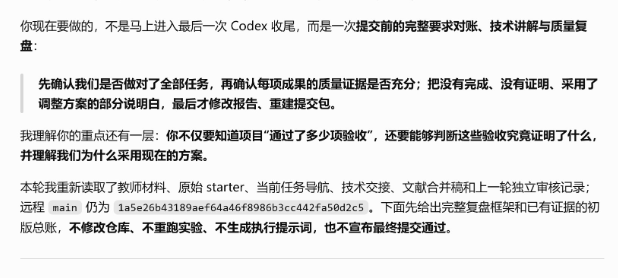
\includegraphics[width=136.500mm]{assets/crops/E20_01_02.png}};
\node[anchor=north west,inner sep=0,text width=36.40mm,align=left] at (159.60,54.63) {\color{Blue}\fontsize{9.5}{13}\selectfont \bfseries 把清单讲成具体方法};
\node[anchor=north west,inner sep=0,text width=36.40mm,align=left] at (159.60,63.28) {\color{Ink}\fontsize{8.7}{12.8}\selectfont  我需要知道为什么这样处理、为什么采用或回退，以及报告还需要怎样完善。GPT据此组织了分块讲解。};
\draw[draw=Blue,line width=.66pt,rounded corners=1mm,-{Stealth[length=1.8mm,width=1.35mm]}] (157.400,58.128) -- (153.200,58.128) -- (153.200,86.291) -- (98.374,86.291);
\draw[Rule,line width=.35pt] (14,283)--(196,283);
\node[anchor=north west,inner sep=0,text width=170.00mm,align=left] at (14.00,287.00) {\color{Muted}\fontsize{6.7}{8.5}\selectfont  智慧城市与位置服务  /  实验一过程报告  /  Part II};
\node[anchor=north west,inner sep=0,text width=11.00mm,align=left] at (185.00,286.50) {\color{Muted}\fontsize{8}{9}\selectfont  64};
\PageEnd

\PageStart
\node[anchor=north west,inner sep=0,text width=182.00mm,align=left] at (14.00,11.00) {\color{Blue}\fontsize{7.8}{10}\selectfont \bfseries PART II · 实验一中的交互与决策  /  理解验收与报告表达的形成};
\node[anchor=north west,inner sep=0,text width=182.00mm,align=left] at (14.00,22.00) {\color{Ink}\fontsize{17.5}{22.5}\selectfont \bfseries 完成研究后，我要求逐项讲清方法与结果（续）};
\node[anchor=north west,inner sep=0,text width=182.00mm,align=left] at (14.00,33.51) {\color{Muted}\fontsize{8.2}{11}\selectfont  接前页，继续阅读这组对话。};
\node[anchor=north west,inner sep=0,text width=136.50mm,align=left] at (14.00,42.51) {\color{Muted}\fontsize{7.2}{9.5}\selectfont  GPT把复盘拆成关联的问题 · 续页};
\node[anchor=north west,inner sep=0] at (14.000,46.709) {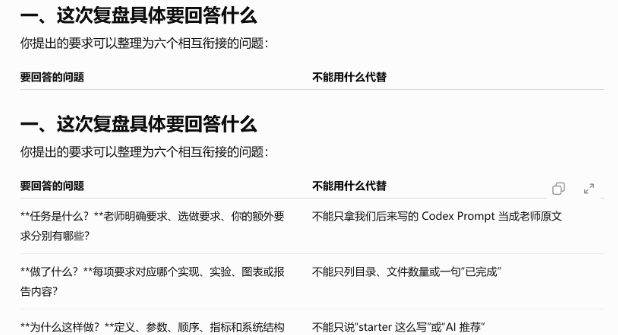
\includegraphics[width=136.500mm]{assets/crops/E20_02_01.png}};
\node[anchor=north west,inner sep=0,text width=136.50mm,align=left] at (14.00,125.90) {\color{Muted}\fontsize{7.2}{9.5}\selectfont  后续：我要求四块完整复盘};
\node[anchor=north west,inner sep=0] at (14.000,130.102) {
\includegraphics[width=136.500mm]{assets/crops/E20_02_02.png}};
\node[anchor=north west,inner sep=0,text width=36.40mm,align=left] at (159.60,48.51) {\color{Blue}\fontsize{9.5}{13}\selectfont \bfseries 串起方法与结果};
\node[anchor=north west,inner sep=0,text width=36.40mm,align=left] at (159.60,57.16) {\color{Ink}\fontsize{8.7}{12.8}\selectfont  这轮讲解发生在主要实验之后，把任务、处理与评价、系统实验、报告交付放在一起，帮助我逐项审阅。};
\draw[draw=Blue,line width=.66pt,rounded corners=1mm,-{Stealth[length=1.8mm,width=1.35mm]}] (157.400,52.009) -- (153.200,52.009) -- (153.200,141.064) -- (143.453,141.064);
\draw[Rule,line width=.35pt] (14,283)--(196,283);
\node[anchor=north west,inner sep=0,text width=170.00mm,align=left] at (14.00,287.00) {\color{Muted}\fontsize{6.7}{8.5}\selectfont  智慧城市与位置服务  /  实验一过程报告  /  Part II};
\node[anchor=north west,inner sep=0,text width=11.00mm,align=left] at (185.00,286.50) {\color{Muted}\fontsize{8}{9}\selectfont  65};
\PageEnd

\PageStart
\node[anchor=north west,inner sep=0,text width=182.00mm,align=left] at (14.00,11.00) {\color{Blue}\fontsize{7.8}{10}\selectfont \bfseries PART II · 实验一中的交互与决策  /  理解验收与报告表达的形成};
\node[anchor=north west,inner sep=0,text width=182.00mm,align=left] at (14.00,22.00) {\color{Ink}\fontsize{17.5}{22.5}\selectfont \bfseries 从技术核查转向报告审阅};
\node[anchor=north west,inner sep=0,text width=182.00mm,align=left] at (14.00,33.51) {\color{Ink}\fontsize{9.5}{14.6}\selectfont  检查技术结果后，我继续审阅报告，重点看叙述主体、方法解释和图文关系。我要求GPT按教师阅读的顺序重新组织内容，把工程管理信息放回相应说明。};
\node[anchor=north west,inner sep=0] at (14,8) {\hypertarget{E21}{}};
\node[anchor=north west,inner sep=0,text width=136.50mm,align=left] at (14.00,48.63) {\color{Muted}\fontsize{7.2}{9.5}\selectfont  我通过技术部分，但要求审阅报告};
\node[anchor=north west,inner sep=0] at (14.000,52.828) {
\includegraphics[width=136.500mm]{assets/crops/E21_01_01.png}};
\node[anchor=north west,inner sep=0,text width=136.50mm,align=left] at (14.00,99.33) {\color{Muted}\fontsize{7.2}{9.5}\selectfont  我具体指出文风、主体和图表问题};
\node[anchor=north west,inner sep=0] at (14.000,103.533) {
\includegraphics[width=136.500mm]{assets/crops/E21_01_02.png}};
\node[anchor=north west,inner sep=0,text width=36.40mm,align=left] at (159.60,54.63) {\color{Blue}\fontsize{9.5}{13}\selectfont \bfseries 继续检查正文与图表};
\node[anchor=north west,inner sep=0,text width=36.40mm,align=left] at (159.60,63.28) {\color{Ink}\fontsize{8.7}{12.8}\selectfont  技术核查之后，我提出还要直接阅读报告，检查文字怎样解释问题、方法与结果，以及图能否帮助理解。};
\draw[draw=Blue,line width=.66pt,rounded corners=1mm,-{Stealth[length=1.8mm,width=1.35mm]}] (157.400,58.128) -- (153.200,58.128) -- (153.200,69.286) -- (106.291,69.286);
\draw[Rule,line width=.35pt] (14,283)--(196,283);
\node[anchor=north west,inner sep=0,text width=170.00mm,align=left] at (14.00,287.00) {\color{Muted}\fontsize{6.7}{8.5}\selectfont  智慧城市与位置服务  /  实验一过程报告  /  Part II};
\node[anchor=north west,inner sep=0,text width=11.00mm,align=left] at (185.00,286.50) {\color{Muted}\fontsize{8}{9}\selectfont  66};
\PageEnd

\PageStart
\node[anchor=north west,inner sep=0,text width=182.00mm,align=left] at (14.00,11.00) {\color{Blue}\fontsize{7.8}{10}\selectfont \bfseries PART II · 实验一中的交互与决策  /  理解验收与报告表达的形成};
\node[anchor=north west,inner sep=0,text width=182.00mm,align=left] at (14.00,22.00) {\color{Ink}\fontsize{17.5}{22.5}\selectfont \bfseries 从技术核查转向报告审阅（续）};
\node[anchor=north west,inner sep=0,text width=182.00mm,align=left] at (14.00,33.51) {\color{Muted}\fontsize{8.2}{11}\selectfont  接前页，继续阅读这组对话。};
\node[anchor=north west,inner sep=0,text width=136.50mm,align=left] at (14.00,42.51) {\color{Muted}\fontsize{7.2}{9.5}\selectfont  GPT区分正文与内部追溯材料};
\node[anchor=north west,inner sep=0] at (14.000,46.709) {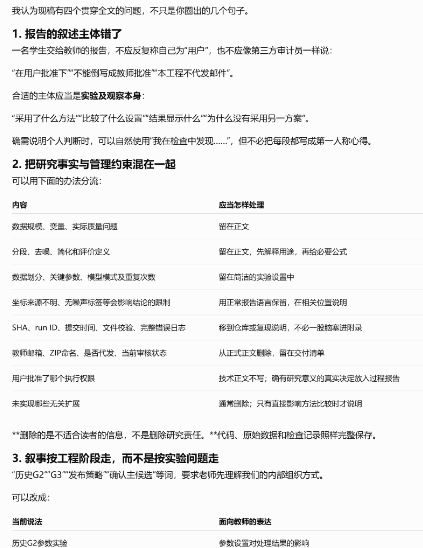
\includegraphics[width=136.500mm]{assets/crops/E21_02_01.png}};
\node[anchor=north west,inner sep=0,text width=36.40mm,align=left] at (159.60,48.51) {\color{Blue}\fontsize{9.5}{13}\selectfont \bfseries 从全文组织入手};
\node[anchor=north west,inner sep=0,text width=36.40mm,align=left] at (159.60,57.16) {\color{Ink}\fontsize{8.7}{12.8}\selectfont  叙述改回我的视角；状态和长哈希移出正文。坐标未注明、缺少真值与边界案例，则用读者能懂的语言保留。};
\draw[draw=Blue,line width=.66pt,rounded corners=1mm,-{Stealth[length=1.8mm,width=1.35mm]}] (157.400,52.009) -- (153.200,52.009) -- (153.200,84.787) -- (114.681,84.787);
\draw[Rule,line width=.35pt] (14,283)--(196,283);
\node[anchor=north west,inner sep=0,text width=170.00mm,align=left] at (14.00,287.00) {\color{Muted}\fontsize{6.7}{8.5}\selectfont  智慧城市与位置服务  /  实验一过程报告  /  Part II};
\node[anchor=north west,inner sep=0,text width=11.00mm,align=left] at (185.00,286.50) {\color{Muted}\fontsize{8}{9}\selectfont  67};
\PageEnd

\PageStart
\node[anchor=north west,inner sep=0,text width=182.00mm,align=left] at (14.00,11.00) {\color{Blue}\fontsize{7.8}{10}\selectfont \bfseries PART II · 实验一中的交互与决策  /  理解验收与报告表达的形成};
\node[anchor=north west,inner sep=0,text width=182.00mm,align=left] at (14.00,22.00) {\color{Ink}\fontsize{17.5}{22.5}\selectfont \bfseries 让研究要求自然进入方法与实验};
\node[anchor=north west,inner sep=0,text width=182.00mm,align=left] at (14.00,33.51) {\color{Ink}\fontsize{9.5}{14.6}\selectfont  修改工程口吻时，我担心审核、量化优化和先单项后组合也被一起删掉。因此我补充：这些要求要自然进入方法与实验，用具体检查、比较和取舍呈现出来。};
\node[anchor=north west,inner sep=0] at (14,8) {\hypertarget{E22}{}};
\node[anchor=north west,inner sep=0,text width=136.50mm,align=left] at (14.00,48.63) {\color{Muted}\fontsize{7.2}{9.5}\selectfont  我要求保留研究要求的实质};
\node[anchor=north west,inner sep=0] at (14.000,52.828) {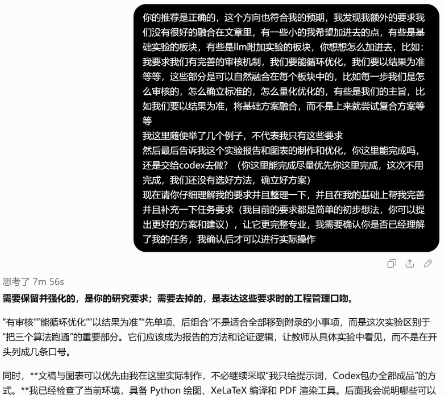
\includegraphics[width=136.500mm]{assets/crops/E22_01_01.png}};
\node[anchor=north west,inner sep=0,text width=136.50mm,align=left] at (14.00,179.23) {\color{Muted}\fontsize{7.2}{9.5}\selectfont  GPT区分内容主线与研究主线};
\node[anchor=north west,inner sep=0] at (14.000,183.426) {
\includegraphics[width=136.500mm]{assets/crops/E22_01_02.png}};
\node[anchor=north west,inner sep=0,text width=36.40mm,align=left] at (159.60,54.63) {\color{Blue}\fontsize{9.5}{13}\selectfont \bfseries 保留要求的实际内容};
\node[anchor=north west,inner sep=0,text width=36.40mm,align=left] at (159.60,63.28) {\color{Ink}\fontsize{8.7}{12.8}\selectfont  我希望读者能看到怎样判断可靠、怎样比较、为什么回退。GPT据此把这些内容放回对应的方法和实验段落。};
\draw[draw=Blue,line width=.66pt,rounded corners=1mm,-{Stealth[length=1.8mm,width=1.35mm]}] (157.400,58.128) -- (153.200,58.128) -- (153.200,94.146) -- (120.201,94.146);
\draw[Rule,line width=.35pt] (14,283)--(196,283);
\node[anchor=north west,inner sep=0,text width=170.00mm,align=left] at (14.00,287.00) {\color{Muted}\fontsize{6.7}{8.5}\selectfont  智慧城市与位置服务  /  实验一过程报告  /  Part II};
\node[anchor=north west,inner sep=0,text width=11.00mm,align=left] at (185.00,286.50) {\color{Muted}\fontsize{8}{9}\selectfont  68};
\PageEnd

\PageStart
\node[anchor=north west,inner sep=0,text width=182.00mm,align=left] at (14.00,11.00) {\color{Blue}\fontsize{7.8}{10}\selectfont \bfseries PART II · 实验一中的交互与决策  /  理解验收与报告表达的形成};
\node[anchor=north west,inner sep=0,text width=182.00mm,align=left] at (14.00,22.00) {\color{Ink}\fontsize{17.5}{22.5}\selectfont \bfseries 让研究要求自然进入方法与实验（续）};
\node[anchor=north west,inner sep=0,text width=182.00mm,align=left] at (14.00,33.51) {\color{Muted}\fontsize{8.2}{11}\selectfont  接前页，继续阅读这组对话。};
\node[anchor=north west,inner sep=0,text width=136.50mm,align=left] at (14.00,42.51) {\color{Muted}\fontsize{7.2}{9.5}\selectfont  GPT区分内容主线与研究主线 · 续页};
\node[anchor=north west,inner sep=0] at (14.000,46.709) {
\includegraphics[width=136.500mm]{assets/crops/E22_02_01.png}};
\node[anchor=north west,inner sep=0,text width=136.50mm,align=left] at (14.00,154.74) {\color{Muted}\fontsize{7.2}{9.5}\selectfont  具体写法：用案例呈现核验与回退};
\node[anchor=north west,inner sep=0] at (14.000,158.943) {
\includegraphics[width=136.500mm]{assets/crops/E22_02_02.png}};
\node[anchor=north west,inner sep=0,text width=36.40mm,align=left] at (159.60,48.51) {\color{Blue}\fontsize{9.5}{13}\selectfont \bfseries 用两条主线组织正文};
\node[anchor=north west,inner sep=0,text width=36.40mm,align=left] at (159.60,57.16) {\color{Ink}\fontsize{8.7}{12.8}\selectfont  GPT把内容主线放在轨迹处理、比较与结果，把研究主线放在验证、取舍与回退。随后用具体案例说明这些要求怎样进入对应段落。};
\draw[draw=Blue,line width=.66pt,rounded corners=1mm,-{Stealth[length=1.8mm,width=1.35mm]}] (157.400,52.009) -- (153.200,52.009) -- (153.200,117.102) -- (149.582,117.102);
\draw[Rule,line width=.35pt] (14,283)--(196,283);
\node[anchor=north west,inner sep=0,text width=170.00mm,align=left] at (14.00,287.00) {\color{Muted}\fontsize{6.7}{8.5}\selectfont  智慧城市与位置服务  /  实验一过程报告  /  Part II};
\node[anchor=north west,inner sep=0,text width=11.00mm,align=left] at (185.00,286.50) {\color{Muted}\fontsize{8}{9}\selectfont  69};
\PageEnd

\PageStart
\node[anchor=north west,inner sep=0,text width=182.00mm,align=left] at (14.00,11.00) {\color{Blue}\fontsize{7.8}{10}\selectfont \bfseries PART II · 实验一中的交互与决策  /  理解验收与报告表达的形成};
\node[anchor=north west,inner sep=0,text width=182.00mm,align=left] at (14.00,22.00) {\color{Ink}\fontsize{17.5}{22.5}\selectfont \bfseries 让研究要求自然进入方法与实验（续）};
\node[anchor=north west,inner sep=0,text width=182.00mm,align=left] at (14.00,33.51) {\color{Muted}\fontsize{8.2}{11}\selectfont  接前页，继续阅读这组对话。};
\node[anchor=north west,inner sep=0,text width=136.50mm,align=left] at (14.00,42.51) {\color{Muted}\fontsize{7.2}{9.5}\selectfont  具体写法：用案例呈现核验与回退 · 续页};
\node[anchor=north west,inner sep=0] at (14.000,46.709) {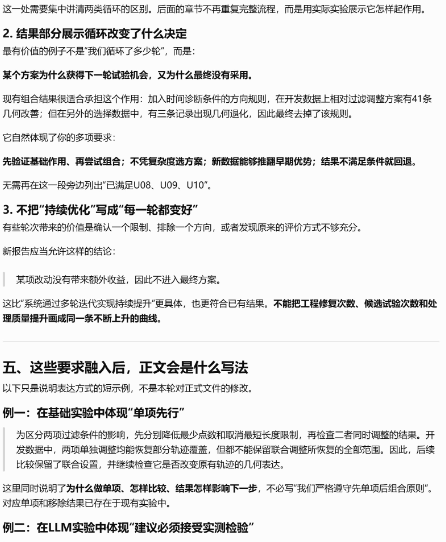
\includegraphics[width=136.500mm]{assets/crops/E22_03_01.png}};
\node[anchor=north west,inner sep=0,text width=36.40mm,align=left] at (159.60,48.51) {\color{Blue}\fontsize{9.5}{13}\selectfont \bfseries 先看具体写法};
\node[anchor=north west,inner sep=0,text width=36.40mm,align=left] at (159.60,57.16) {\color{Ink}\fontsize{8.7}{12.8}\selectfont  GPT用单项验证、共同参考和组合回退给出段落样例。我先检查这种表达，再决定怎样扩展成正式正文。};
\draw[draw=Blue,line width=.66pt,rounded corners=1mm,-{Stealth[length=1.8mm,width=1.35mm]}] (157.400,52.009) -- (153.200,52.009) -- (153.200,165.458) -- (92.044,165.458);
\draw[Rule,line width=.35pt] (14,283)--(196,283);
\node[anchor=north west,inner sep=0,text width=170.00mm,align=left] at (14.00,287.00) {\color{Muted}\fontsize{6.7}{8.5}\selectfont  智慧城市与位置服务  /  实验一过程报告  /  Part II};
\node[anchor=north west,inner sep=0,text width=11.00mm,align=left] at (185.00,286.50) {\color{Muted}\fontsize{8}{9}\selectfont  70};
\PageEnd

\PageStart
\node[anchor=north west,inner sep=0,text width=182.00mm,align=left] at (14.00,11.00) {\color{Blue}\fontsize{7.8}{10}\selectfont \bfseries PART II · 实验一中的交互与决策  /  理解验收与报告表达的形成};
\node[anchor=north west,inner sep=0,text width=182.00mm,align=left] at (14.00,22.00) {\color{Ink}\fontsize{17.5}{22.5}\selectfont \bfseries 用实际文字和图型作出表达选择};
\node[anchor=north west,inner sep=0,text width=182.00mm,align=left] at (14.00,33.51) {\color{Ink}\fontsize{9.5}{14.6}\selectfont  我要求列出需要修改的文字类型，每类提供三种写法，再用真实数据制作候选图。看到具体段落和图形之后，我才能判断阅读效果，并选择适合这份报告的表达。};
\node[anchor=north west,inner sep=0] at (14,8) {\hypertarget{E23}{}};
\node[anchor=north west,inner sep=0,text width=136.50mm,align=left] at (14.00,48.63) {\color{Muted}\fontsize{7.2}{9.5}\selectfont  我要求完整文字与实际图型候选};
\node[anchor=north west,inner sep=0] at (14.000,52.828) {
\includegraphics[width=136.500mm]{assets/crops/E23_01_01.png}};
\node[anchor=north west,inner sep=0,text width=136.50mm,align=left] at (14.00,90.63) {\color{Muted}\fontsize{7.2}{9.5}\selectfont  GPT提供章节与开篇候选};
\node[anchor=north west,inner sep=0] at (14.000,94.825) {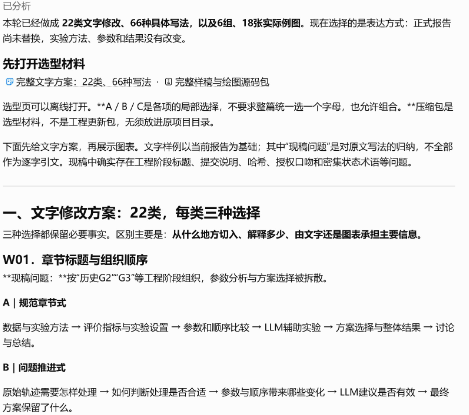
\includegraphics[width=136.500mm]{assets/crops/E23_01_02.png}};
\node[anchor=north west,inner sep=0,text width=36.40mm,align=left] at (159.60,54.63) {\color{Blue}\fontsize{9.5}{13}\selectfont \bfseries 为选择准备实际材料};
\node[anchor=north west,inner sep=0,text width=36.40mm,align=left] at (159.60,63.28) {\color{Ink}\fontsize{8.7}{12.8}\selectfont  GPT提供22类文字、66种写法和6组18幅候选图。我对照具体内容检查不同组织方式，再作选择。};
\draw[draw=Blue,line width=.66pt,rounded corners=1mm,-{Stealth[length=1.8mm,width=1.35mm]}] (157.400,58.128) -- (153.200,58.128) -- (153.200,71.019) -- (104.806,71.019);
\draw[Rule,line width=.35pt] (14,283)--(196,283);
\node[anchor=north west,inner sep=0,text width=170.00mm,align=left] at (14.00,287.00) {\color{Muted}\fontsize{6.7}{8.5}\selectfont  智慧城市与位置服务  /  实验一过程报告  /  Part II};
\node[anchor=north west,inner sep=0,text width=11.00mm,align=left] at (185.00,286.50) {\color{Muted}\fontsize{8}{9}\selectfont  71};
\PageEnd

\PageStart
\node[anchor=north west,inner sep=0,text width=182.00mm,align=left] at (14.00,11.00) {\color{Blue}\fontsize{7.8}{10}\selectfont \bfseries PART II · 实验一中的交互与决策  /  理解验收与报告表达的形成};
\node[anchor=north west,inner sep=0,text width=182.00mm,align=left] at (14.00,22.00) {\color{Ink}\fontsize{17.5}{22.5}\selectfont \bfseries 用实际文字和图型作出表达选择（续）};
\node[anchor=north west,inner sep=0,text width=182.00mm,align=left] at (14.00,33.51) {\color{Muted}\fontsize{8.2}{11}\selectfont  接前页，继续阅读这组对话。};
\node[anchor=north west,inner sep=0,text width=136.50mm,align=left] at (14.00,42.51) {\color{Muted}\fontsize{7.2}{9.5}\selectfont  GPT提供章节与开篇候选 · 续页};
\node[anchor=north west,inner sep=0] at (14.000,46.709) {
\includegraphics[width=136.500mm]{assets/crops/E23_02_01.png}};
\node[anchor=north west,inner sep=0,text width=136.50mm,align=left] at (14.00,105.75) {\color{Muted}\fontsize{7.2}{9.5}\selectfont  我选择问题驱动，保留直接开篇};
\node[anchor=north west,inner sep=0] at (14.000,109.953) {
\includegraphics[width=136.500mm]{assets/crops/E23_02_02.png}};
\node[anchor=north west,inner sep=0,text width=136.50mm,align=left] at (14.00,157.45) {\color{Muted}\fontsize{7.2}{9.5}\selectfont  GPT记录我的组合选择};
\node[anchor=north west,inner sep=0] at (14.000,161.653) {
\includegraphics[width=136.500mm]{assets/crops/E23_02_03.png}};
\node[anchor=north west,inner sep=0,text width=36.40mm,align=left] at (159.60,48.51) {\color{Blue}\fontsize{9.5}{13}\selectfont \bfseries 按不同内容分别选择};
\node[anchor=north west,inner sep=0,text width=36.40mm,align=left] at (159.60,57.16) {\color{Ink}\fontsize{8.7}{12.8}\selectfont  开篇和目录直接交代，主体从问题引出方法。图型分别选择，G6则因看不清逻辑继续修改。};
\draw[draw=Blue,line width=.66pt,rounded corners=1mm,-{Stealth[length=1.8mm,width=1.35mm]}] (157.400,52.009) -- (153.200,52.009) -- (153.200,127.503) -- (103.400,127.503);
\draw[Rule,line width=.35pt] (14,283)--(196,283);
\node[anchor=north west,inner sep=0,text width=170.00mm,align=left] at (14.00,287.00) {\color{Muted}\fontsize{6.7}{8.5}\selectfont  智慧城市与位置服务  /  实验一过程报告  /  Part II};
\node[anchor=north west,inner sep=0,text width=11.00mm,align=left] at (185.00,286.50) {\color{Muted}\fontsize{8}{9}\selectfont  72};
\PageEnd

\PageStart
\node[anchor=north west,inner sep=0,text width=182.00mm,align=left] at (14.00,11.00) {\color{Blue}\fontsize{7.8}{10}\selectfont \bfseries PART II · 实验一中的交互与决策  /  理解验收与报告表达的形成};
\node[anchor=north west,inner sep=0,text width=182.00mm,align=left] at (14.00,22.00) {\color{Ink}\fontsize{17.5}{22.5}\selectfont \bfseries 先审样章，再完成并验收整篇报告};
\node[anchor=north west,inner sep=0,text width=182.00mm,align=left] at (14.00,33.51) {\color{Ink}\fontsize{9.5}{14.6}\selectfont  我对G6的反馈是希望看清核验依据与判断关系。GPT重构样章后，我检查实际页面，再要求整篇沿同一方向完成；完整25页报告交付后，我作出了验收确认。};
\node[anchor=north west,inner sep=0] at (14,8) {\hypertarget{E24}{}};
\node[anchor=north west,inner sep=0,text width=136.50mm,align=left] at (14.00,48.63) {\color{Muted}\fontsize{7.2}{9.5}\selectfont  我对G6的原始反馈};
\node[anchor=north west,inner sep=0] at (14.000,52.828) {
\includegraphics[width=136.500mm]{assets/crops/E24_01_01.png}};
\node[anchor=north west,inner sep=0,text width=136.50mm,align=left] at (14.00,100.33) {\color{Muted}\fontsize{7.2}{9.5}\selectfont  样章：核验逻辑与历史归属纠正};
\node[anchor=north west,inner sep=0] at (14.000,104.528) {
\includegraphics[width=136.500mm]{assets/crops/E24_01_02.png}};
\node[anchor=north west,inner sep=0,text width=36.40mm,align=left] at (159.60,54.63) {\color{Blue}\fontsize{9.5}{13}\selectfont \bfseries 我要求看清核验逻辑};
\node[anchor=north west,inner sep=0,text width=36.40mm,align=left] at (159.60,63.28) {\color{Ink}\fontsize{8.7}{12.8}\selectfont  在报告图形审阅中，我指出框架过于简朴、关系不清楚，要求把检查依据和判断过程表达出来。};
\draw[draw=Blue,line width=.66pt,rounded corners=1mm,-{Stealth[length=1.8mm,width=1.35mm]}] (157.400,58.128) -- (153.200,58.128) -- (153.200,79.378) -- (119.600,79.378);
\node[anchor=north west,inner sep=0,text width=36.40mm,align=left] at (159.60,100.37) {\color{Violet}\fontsize{9.5}{13}\selectfont \bfseries 用具体关系重画G6};
\node[anchor=north west,inner sep=0,text width=36.40mm,align=left] at (159.60,109.02) {\color{Ink}\fontsize{8.7}{12.8}\selectfont  GPT把共同原始参考、候选结果和分层检查画清楚。记录7764的实际核验为这张技术说明图提供了案例。};
\draw[draw=Violet,line width=.66pt,rounded corners=1mm,-{Stealth[length=1.8mm,width=1.35mm]}] (157.400,103.872) -- (155.300,103.872) -- (155.300,181.628) -- (146.600,181.628);
\draw[Rule,line width=.35pt] (14,283)--(196,283);
\node[anchor=north west,inner sep=0,text width=170.00mm,align=left] at (14.00,287.00) {\color{Muted}\fontsize{6.7}{8.5}\selectfont  智慧城市与位置服务  /  实验一过程报告  /  Part II};
\node[anchor=north west,inner sep=0,text width=11.00mm,align=left] at (185.00,286.50) {\color{Muted}\fontsize{8}{9}\selectfont  73};
\PageEnd

\PageStart
\node[anchor=north west,inner sep=0,text width=182.00mm,align=left] at (14.00,11.00) {\color{Blue}\fontsize{7.8}{10}\selectfont \bfseries PART II · 实验一中的交互与决策  /  理解验收与报告表达的形成};
\node[anchor=north west,inner sep=0,text width=182.00mm,align=left] at (14.00,22.00) {\color{Ink}\fontsize{17.5}{22.5}\selectfont \bfseries 先审样章，再完成并验收整篇报告（续）};
\node[anchor=north west,inner sep=0,text width=182.00mm,align=left] at (14.00,33.51) {\color{Muted}\fontsize{8.2}{11}\selectfont  接前页，继续阅读这组对话。};
\node[anchor=north west,inner sep=0,text width=136.50mm,align=left] at (14.00,42.51) {\color{Muted}\fontsize{7.2}{9.5}\selectfont  我确认样章并要求完整重构};
\node[anchor=north west,inner sep=0] at (14.000,46.709) {
\includegraphics[width=136.500mm]{assets/crops/E24_02_01.png}};
\node[anchor=north west,inner sep=0,text width=136.50mm,align=left] at (14.00,72.91) {\color{Muted}\fontsize{7.2}{9.5}\selectfont  完整报告交付后：我明确验收};
\node[anchor=north west,inner sep=0] at (14.000,77.109) {
\includegraphics[width=136.500mm]{assets/crops/E24_02_02.png}};
\node[anchor=north west,inner sep=0,text width=136.50mm,align=left] at (14.00,122.38) {\color{Muted}\fontsize{7.2}{9.5}\selectfont  GPT承接验收并限定规则更新};
\node[anchor=north west,inner sep=0] at (14.000,126.583) {
\includegraphics[width=136.500mm]{assets/crops/E24_02_03.png}};
\node[anchor=north west,inner sep=0,text width=36.40mm,align=left] at (159.60,48.51) {\color{Blue}\fontsize{9.5}{13}\selectfont \bfseries 从样章到全篇};
\node[anchor=north west,inner sep=0,text width=36.40mm,align=left] at (159.60,57.16) {\color{Ink}\fontsize{8.7}{12.8}\selectfont  我确认实际样章后要求完整重构，随后审阅并验收25页实验报告。GPT再将这些表达做法整理为可复用原则。};
\draw[draw=Blue,line width=.66pt,rounded corners=1mm,-{Stealth[length=1.8mm,width=1.35mm]}] (157.400,52.009) -- (153.200,52.009) -- (153.200,141.923) -- (33.411,141.923);
\node[anchor=north west,inner sep=0,text width=36.40mm,align=left] at (159.60,98.77) {\color{Rose}\fontsize{8.9}{12.5}\selectfont \bfseries 我的回看};
\node[anchor=north west,inner sep=0,text width=36.40mm,align=left] at (159.60,105.77) {\color{Ink}\fontsize{8.5}{12.7}\selectfont  验收成品后，我和GPT将问题驱动写作、图文对应，以及已验收源文件的保护方式整理为后续可复用的规则。};
\draw[Rule,line width=.35pt] (14,283)--(196,283);
\node[anchor=north west,inner sep=0,text width=170.00mm,align=left] at (14.00,287.00) {\color{Muted}\fontsize{6.7}{8.5}\selectfont  智慧城市与位置服务  /  实验一过程报告  /  Part II};
\node[anchor=north west,inner sep=0,text width=11.00mm,align=left] at (185.00,286.50) {\color{Muted}\fontsize{8}{9}\selectfont  74};
\PageEnd

\PageStart
\node[anchor=north west,inner sep=0,text width=182.00mm,align=left] at (14.00,11.00) {\color{Blue}\fontsize{7.8}{10}\selectfont \bfseries PART II · 实验一中的交互与决策  /  理解验收与报告表达的形成  /  关系图};
\node[anchor=north west,inner sep=0,text width=182.00mm,align=left] at (14.00,25.00) {\color{Ink}\fontsize{18}{24}\selectfont \bfseries 我的报告审阅怎样落实到成品};
\node[anchor=north west,inner sep=0,text width=182.00mm,align=left] at (14.00,43.00) {\color{Ink}\fontsize{9.6}{15}\selectfont  我先指出文字和图形的问题，再看具体候选与样章，确认表达方向后完成整篇报告。};
\node[anchor=north west,inner sep=0] at (14,71) {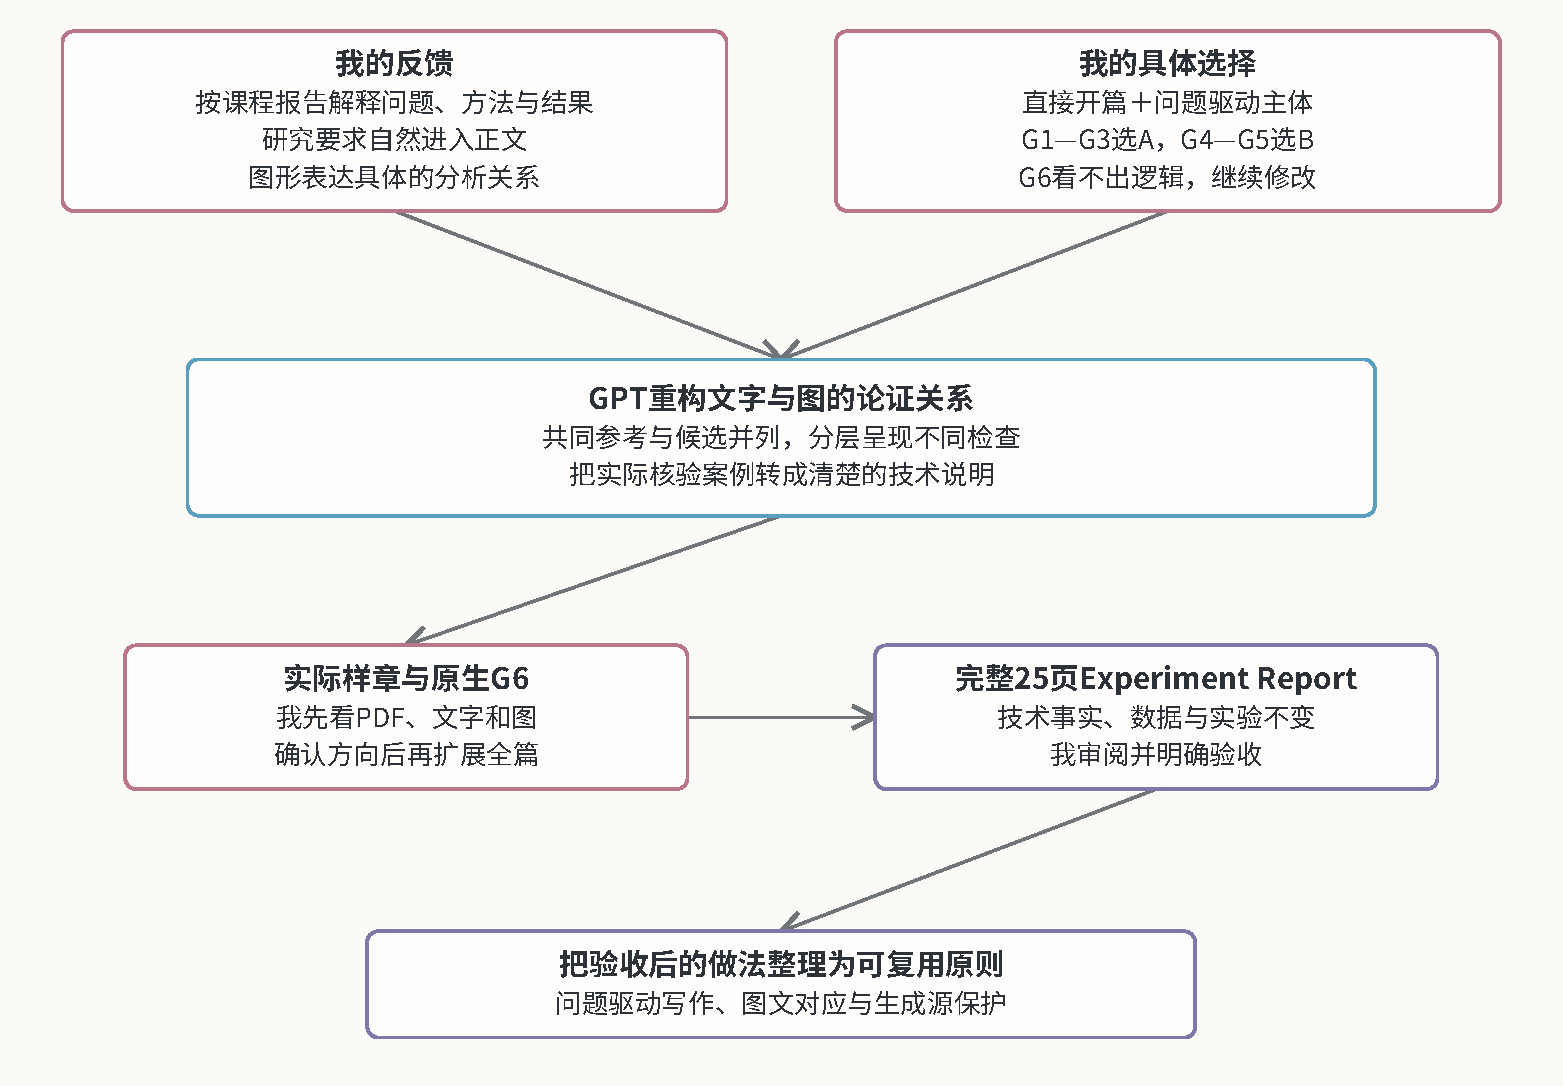
\includegraphics[width=182mm]{figures/D05.pdf}};
\node[anchor=north west,inner sep=0,text width=182.00mm,align=left] at (14.00,207.49) {\color{Ink}\fontsize{10}{15.5}\selectfont  G6的修改来自我的图形审阅，记录7764的实际核验提供了技术案例。样章确认后，GPT将相同表达方向扩展到全篇，我再审阅完整成品。};
\draw[Rule,line width=.35pt] (14,283)--(196,283);
\node[anchor=north west,inner sep=0,text width=170.00mm,align=left] at (14.00,287.00) {\color{Muted}\fontsize{6.7}{8.5}\selectfont  智慧城市与位置服务  /  实验一过程报告  /  Part II};
\node[anchor=north west,inner sep=0,text width=11.00mm,align=left] at (185.00,286.50) {\color{Muted}\fontsize{8}{9}\selectfont  75};
\PageEnd

\PageStart
\node[anchor=north west,inner sep=0,text width=182.00mm,align=left] at (14.00,11.00) {\color{Rose}\fontsize{8}{11}\selectfont \bfseries 整体工作流回顾};
\node[anchor=north west,inner sep=0,text width=182.00mm,align=left] at (14.00,25.00) {\color{Ink}\fontsize{18}{24}\selectfont \bfseries 回到我最初要求的“真实完成与持续改进”};
\node[anchor=north west,inner sep=0,text width=182.00mm,align=left] at (14.00,45.00) {\color{Ink}\fontsize{9.6}{15}\selectfont  回看这次实验，我最关心的几件事始终连在一起：依据是否清楚，任务有没有实际执行，结果怎样核验，以及发现问题后能否继续推进。下面回引我当时的要求，再看它怎样逐步落实。};
\node[anchor=north west,inner sep=0] at (14,74) {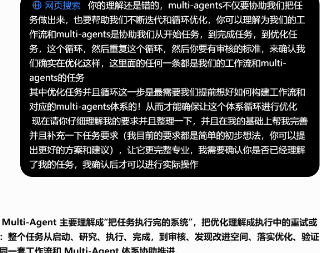
\includegraphics[width=136.5mm]{assets/crops/closing_user.png}};
\node[anchor=north west,inner sep=0,text width=36.40mm,align=left] at (159.60,78.00) {\color{Blue}\fontsize{9.5}{13}\selectfont \bfseries 让反馈引出下一步};
\node[anchor=north west,inner sep=0,text width=36.40mm,align=left] at (159.60,96.00) {\color{Ink}\fontsize{8.8}{13}\selectfont  我要求体系完成任务后继续检查结果、寻找改进。后续讨论又明确了候选依据、有限预算和停止条件。};
\node[anchor=north west,inner sep=0,text width=182.00mm,align=left] at (14.00,207.00) {\color{Ink}\fontsize{10}{15.5}\selectfont  我在这次任务中不断补充和修正要求：把Multi-Agent拉回真实轨迹任务，要求先验证单项、共用评价，让普通修复留在当前Goal，并继续检查方法解释与报告表达。GPT负责研究、解释、候选和结果核查，Codex负责实现与运行；我的质疑和选择也持续影响着后续工作。};
\node[anchor=north west,inner sep=0,text width=182.00mm,align=left] at (14.00,245.00) {\color{Ink}\fontsize{10}{15.5}\selectfont  前期交接曾经反复，审核接口出现过漏洞，开发阶段有优势的组合也在新记录上退出。正是这些经历，让我们逐渐明确什么时候继续、怎样修复，以及为什么保留较简单的方案。};
\draw[Rule,line width=.35pt] (14,283)--(196,283);
\node[anchor=north west,inner sep=0,text width=170.00mm,align=left] at (14.00,287.00) {\color{Muted}\fontsize{6.7}{8.5}\selectfont  智慧城市与位置服务  /  实验一过程报告  /  回顾};
\node[anchor=north west,inner sep=0,text width=11.00mm,align=left] at (185.00,286.50) {\color{Muted}\fontsize{8}{9}\selectfont  76};
\PageEnd

\PageStart
\node[anchor=north west,inner sep=0,text width=182.00mm,align=left] at (14.00,11.00) {\color{Rose}\fontsize{8}{11}\selectfont \bfseries 整体工作流回顾  /  研究演化图};
\node[anchor=north west,inner sep=0,text width=182.00mm,align=left] at (14.00,25.00) {\color{Ink}\fontsize{18}{24}\selectfont \bfseries 从共同基础到实验一，工作流怎样改变};
\node[anchor=north west,inner sep=0,text width=182.00mm,align=left] at (14.00,47.00) {\color{Ink}\fontsize{9.6}{15}\selectfont  回看整个过程，我的几次关键补充逐渐把研究判断、实际执行、核验和任务恢复接在一起。};
\node[anchor=north west,inner sep=0] at (14,78) {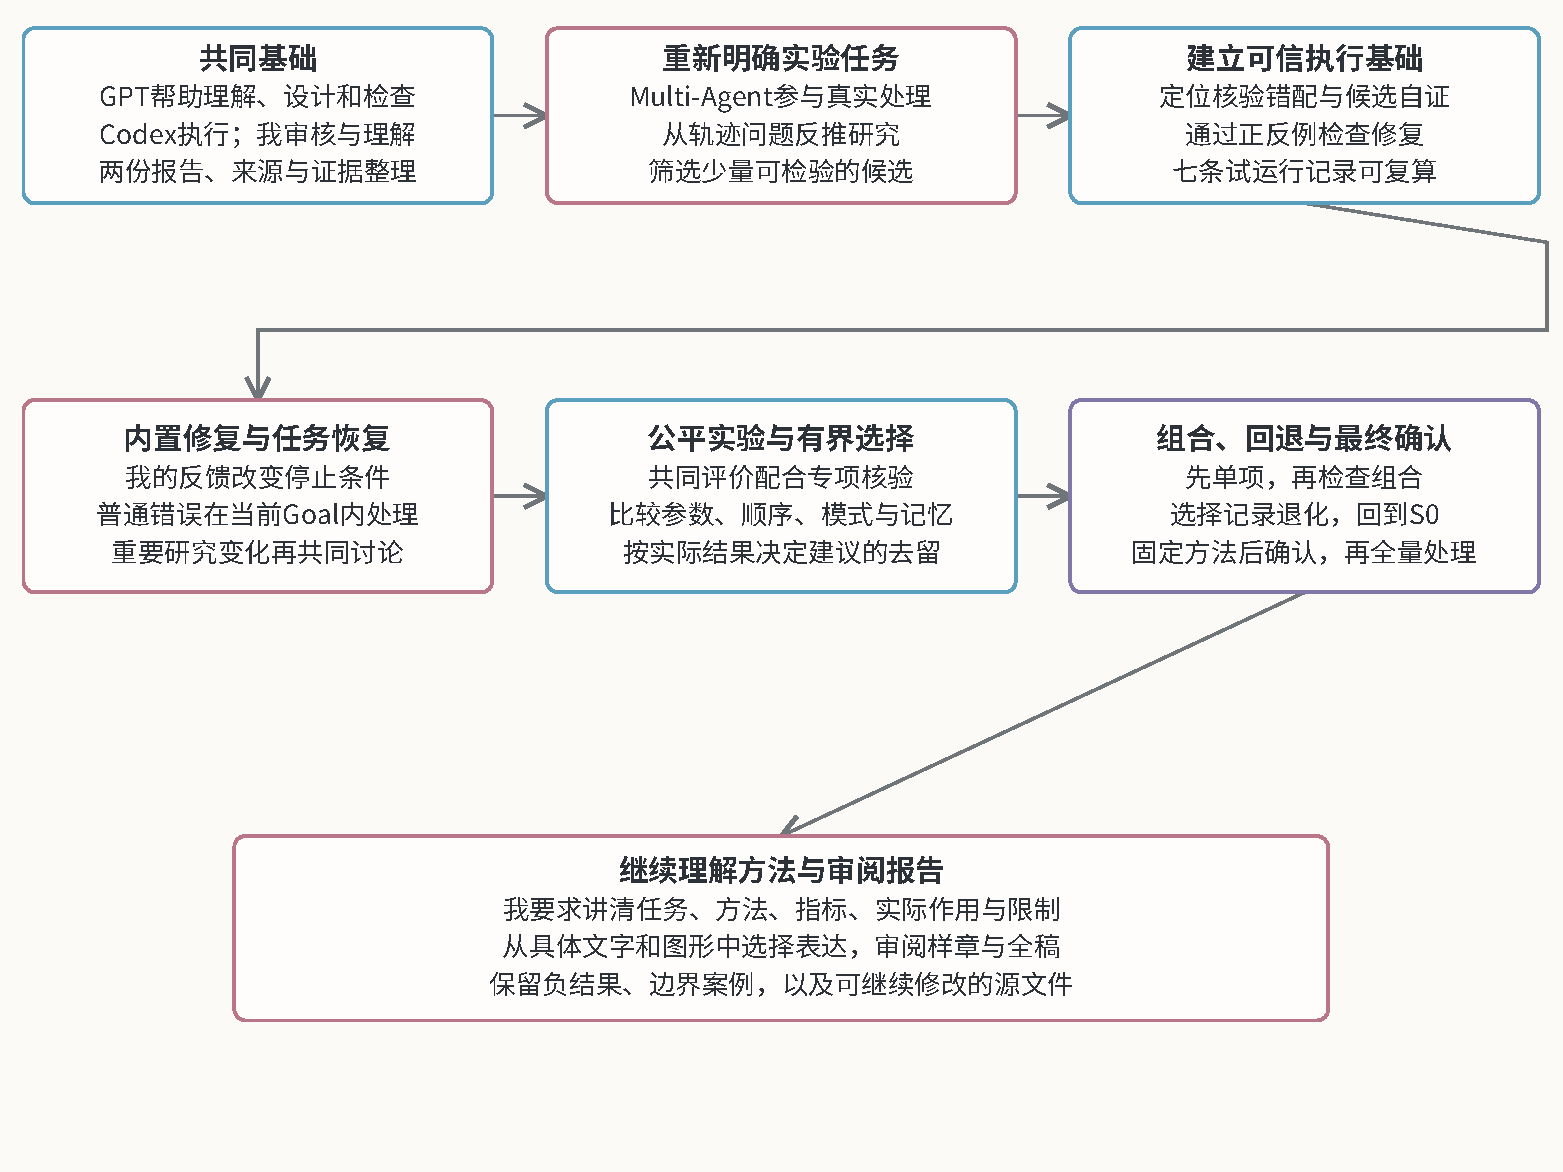
\includegraphics[width=182mm]{figures/D06.pdf}};
\node[anchor=north west,inner sep=0,text width=182.00mm,align=left] at (14.00,224.00) {\color{Ink}\fontsize{10}{15.5}\selectfont  这次交互让我形成了更具体的工作习惯：先把问题和依据讲清，再用可检查的结果决定下一步；实现有错就修复，有效候选没有收益就保留结论并调整方向。方案和报告都在这种往返中逐步成形。};
\node[anchor=north west,inner sep=0,text width=182.00mm,align=left] at (14.00,251.00) {\color{Muted}\fontsize{8.8}{13}\selectfont  相关材料：原始对话节选见各章；算法、指标与完整结果见配套Experiment Report；截图来源、裁切与箭头定义、构建方法和制作记录随LaTeX源包保存。};
\draw[Rule,line width=.35pt] (14,283)--(196,283);
\node[anchor=north west,inner sep=0,text width=170.00mm,align=left] at (14.00,287.00) {\color{Muted}\fontsize{6.7}{8.5}\selectfont  智慧城市与位置服务  /  实验一过程报告  /  回顾};
\node[anchor=north west,inner sep=0,text width=11.00mm,align=left] at (185.00,286.50) {\color{Muted}\fontsize{8}{9}\selectfont  77};
\PageEnd

\end{document}
